\documentclass[11pt, ngerman,english,a4]{article}
\usepackage[bottom,flushmargin,hang,multiple]{footmisc}

\usepackage[T1]{fontenc}
\usepackage{babel}
\usepackage[utf8]{inputenc}
\usepackage{xcolor} % to highlight text
\usepackage{setspace} % to doublespace
\usepackage[margin=1in]{geometry}
\usepackage[]{hyperref}
\usepackage{graphicx}
\usepackage{caption}
\usepackage{subcaption}
\usepackage{multicol}
\usepackage{amsmath, amssymb}
\usepackage{booktabs}
\usepackage{multirow}
\usepackage{color,soul}
\usepackage{bm}
\usepackage[russian]{babel}
\usepackage[sort&compress]{natbib} 
\usepackage{newpxtext,newpxmath}

\usepackage{float}
\usepackage[labelfont=bf,textfont=md]{caption}
\usepackage{mdframed}
\usepackage{lscape}
\usepackage{ragged2e}
%\usepackage{MnSymbol}
\sethlcolor{lightgray}
\widowpenalty10000
\clubpenalty10000
\hyphenpenalty100
\usepackage[page,header]{appendix}
\usepackage{titletoc}
\usepackage{subfiles} % Best loaded last in the preamble
\usepackage{threeparttable}

\makeatletter
  \providecommand*\setfloatlocations[2]{\@namedef{fps@#1}{#2}}
\makeatother
\setfloatlocations{figure}{htbp}
\setfloatlocations{table}{htbp}


\usepackage{tikz, siunitx}
\usetikzlibrary{positioning}
\tikzset{mynode/.style={draw,text width=1.5in,align=center}
}

\setcitestyle{authoryear,open={(},close={)}}

\author{
	Lion Behrens\\University of Mannheim\\behrens@uni-mannheim.de\\
	\and
	Viktoriia Semenova\\University of Mannheim\\semenova@uni-mannheim.de
}

\date{\today }

\title{Election Fraud Information, Punishment, and Political Trust: Evidence from a Survey Experiment in Colombia, Mexico, and Russia\footnote{This paper has been presented at the 11th Annual Conference of the European Political Science Association (EPSA) and the University of Mannheim's CDSS workshop `Political Science'. We are grateful to Harald Schoen, Thomas Bräuninger, Thomas Gschwend as well as all panel and workshop participants for helpful comments on previous versions of this manuscript. This research was supported by the University of Mannheim's Graduate School of Economic and Social Sciences (GESS).}\vspace{0.7cm}} 

 

\begin{document}
\maketitle
\thispagestyle{empty}

\onehalfspacing


\noindent \textbf{Abstract:} Scholars have shown that consciousness of election fraud lets individuals withdraw support from candidates, institutions and governments that are supposedly involved in manipulation. We argue that election fraud information will let individuals extrapolate legitimacy loss even to political institutions that are unrelated to electoral events and lead to decays of trust in the political system as a whole. Second, we argue that these spillovers are crucially shaped by the reactions of other political actors. Within-system corrections like court punishments of alleged fraud perpetrators can mitigate decays in diffuse support. We present evidence for these expectations from a pre-registered online survey experiment in Colombia, Mexico and Russia. Our findings hold important implications for the study of developing democracies and electoral autocracies.


\vspace{1cm}

\noindent \textbf{Keywords:} \textit{Election Fraud; Diffuse Support; Political Trust; Electoral Courts; Survey Experiment; Causal estimation.} \\ 



\newpage
\setcounter{page}{1}
\doublespacing

\section*{Introduction}

Which consequences do information about electoral fraud have for citizens' relationship towards their political system? Since the `electoral revolution' that surged since the mid-twentieth century led to a dramatic increase in the number of electoral events (\citealt{Norris2014}), multiparty elections have become omnipresent across new democracies and electoral authoritarian regimes worldwide. The conduct of these, however, is frequently accompanied by publicly voiced doubts about their integrity. For instance, nearly 80\% of all federal elections in non-established democracies nowadays are monitored `on the ground' by international observers (\citealt{Kelley2012a}; \citealt{Hyde2011}) and around half of all observed elections had led international missions to declare problems of moderate or high magnitude (\citealt{Kelley2012a, Kelley2012b}). Additionally, a growing number of academic researchers dissect fine-graded voting returns using statistical methodology that is designed to flag numerical peculiarities which are indicative of systematic interference. After the 2019 election in Bolivia, for instance, this interplay has led the incumbent president Evo Morales to step down from office after the Department for Electoral Cooperation and Observation of the Organization of American States has voiced criticisms around statistical patterns among late-counted votes (\citealt{OAS2019}; \citealt{Idrobo2020}).

Among the citizens themselves, credible information about electoral crimes can hold several behavioral and attitudinal consequences. Becoming conscious of electoral malpractice has been shown to lead to participation in popular protests and violent uprisings (\citealt{Daxecker2012}). The literature has furthermore amassed a wealth of knowledge on the effects of election fraud perceptions on individuals' attitudes towards their political authorities. First, scholars have examined how information about electoral misconduct shape individuals' evaluations of the electoral process itself.  For instance, \citet{Robertson2017} shows that providing citizens with critical reports of election observation missions considerably reduces their perceived levels of electoral integrity. Second, citizens that are conscious about misbehavior withdraw support from those candidates that are allegedly involved in malpractice (\citealt{Reuter2019}) and express lower levels of legitimacy for the political regime that surged out of an electoral process that is perceived to be fraudulent (\citealt{Williamson2021}).

This article holds two main contributions. First, we draw on theories of information processing and outline a mechanism of \textit{attitudinal spillover} which states that individuals extrapolate specific fraud allegations to their confidence in the political system itself. The theory argues that even when information about fraud is attributed to unique political actors, citizens tend to relate these to political institutions that are unconnected to electoral administration. In contrast to the prior literature, the presence of such attitudinal spillovers predicts that consciousness about electoral misconduct will not let individuals merely detach from political authorities that can be directly linked to misbehavior and the regime that surged out of an illegitimate election process, but rather holds implications that are considerably more detrimental. Following the mechanism that we outline, consciousness about electoral malpractice can lead citizens to withdraw approval from the political system as a whole.

Second, we argue that the spillover effect induced by fraud information is endogenous to the reactions of other actors of the political system. The underlying assumption is that attitude shifts as a consequence to fraud information do not appear in isolation---they can be exacerbated or mitigated by how other political actors respond. For instance, alleged perpetrators being removed from their posts in the electoral commission or public court rulings on electoral crimes may send out signals of the political system's professionalism, autonomy, and commitment to a fair electoral process  (\citealt{Kerr2020}). Hence, successful convictions of alleged perpetrators might therefore function as signals of at least some level of horizontal `checks and balances', mitigating individuals' depressed levels of diffuse support. Grasping such dynamics is crucial for understanding the real-life impact of fraud information, as citizens are not only exposed to disseminated information about electoral malpractice, but also perceive how actors of the political system \textit{respond}.

We present evidence from a pre-registered online survey experiment conducted in Colombia, Mexico and Russia ($n=2,057$) assessing (i) the presence of attitudinal spillovers of election fraud information to political institutions that are unrelated to electoral events and (ii) how punishment of alleged perpetrators exacerbate or mitigate decays in political trust. Since much of the previous literature has focused on the analysis of large cross-national survey data, our empirical analysis first showcases that these are unable to answer questions such as those that we pose here using 48,953 respondents across 48 countries from Wave 7 (2017-2020) of the World Values Survey (WVS). Even after applying a range of state-of-the-art matching algorithms for causal estimation combined with various robustness checks and a Bayesian estimation approach, we cannot distinguish spillover effects on political institutions (that are dictated by theory) from spillovers on non-political institutions (that should not be present in theory). We then present evidence from our experiment adding two original findings to the current literature. First, exposing individuals to information about electoral misconduct induces negative spillovers to trust in components of the political system that are not tied to elections. Second, disseminating information on punishments of alleged perpetrators does mitigate, but not remove, decays in diffuse support. Government supporters as well as opponents are affected alike. 

The main conclusion of our article is that the consequences of administering election fraud for public support are even more detrimental than currently acknowledged by the literature. On the one hand, this is because information on electoral misconduct even induces shifts in public support towards components of the political system that are no beneficiaries of manipulation and are not related to the administration of electoral administration in the first place. On the other hand, this is because once fraud information is disseminated, even credible punishments cannot completely account for the loss of trust in the political system. Hence, our findings cast doubt on the effectiveness of strategies described as `blame attribution' (\citealt{Beazer2019}; \citealt{Rozenas2019b}) in the literature on authoritarianism. Regimes that aim to prevent popular disapproval and use punishments to shift responsibilities for misconduct away from the regime and towards micro-level agents who are convicted for criminal activities can only expect limited success. Additionally, this article speaks to the literature on statistical detection of election fraud. Researchers and practitioners need to be careful not to produce false-positive claims, as the loss in political trust (i) even extrapolates to components of the political system that are unrelated to electoral administration (ii) and can hardly be restored. 


\section*{Election Fraud Information and Political Trust}

In this section, we outline a theory of how the acquisition of new information about the integrity of domestic elections will affect the amount of trust that citizens place in the institutions of their broader political system. Essentially, this comes down to defining an argument of why individuals will extrapolate information about electoral misconduct to political institutions that are unrelated to electoral administration. Afterwards, we discuss how the interventions of other political actors can mitigate such spillover effects.

\subsection*{Election Fraud Information and Attitude Extrapolation}

Scholarly contributions that examine the attitudinal nexus between citizens and the state commonly refer to the work of  David \citet{Easton1965, Easton1975} on ‘system support' as a joint conceptual heritage. The theoretical distinction that is most relevant for our argument is the classical discrimination between diffuse and specific levels of support. Specific support refers to the relationship between members of a system and the specific actions and decisions of political authorities that reside within its institutions. As such, specific support relates to the evaluations of the day-to-day actions of political leaders, and are highest if perceived outputs match citizens' articulated demands (\citealt{Easton1975}, p. 438). In contrast, diffuse support describes individuals' generalized attachment to the political system. According to Easton, \textit{"[diffuse support] refers to evaluations of what an object is or represents [..] not of what it does. [..] Whereas specific support is extended only to the incumbent authorities, diffuse support is directed towards offices themselves as well as their individual occupants. More than that, diffuse support is support that underlies the regime as a whole and the political community."} (\citealt{Easton1975}, pp. 444-445). Hence, diffuse support is \textit{a priori} expected to be more durable than citizens' performance evaluation of specific political authorities. While positive evaluations of actors' performance is volatile and comes with consistent rise and fall, diffuse political support for the entity of the political system is in general thought to be long-lasting. 

Early work on the concept of political support did almost exclusively focus on the relation between citizens and the state in the context of the United States and other advanced industrialized democracies (\citealt{Easton1965, Easton1975}; \citealt{Citrin1974}). Importantly, already in their seminal work on popular support for authoritarian regimes, \citet{Geddes1989} have argued that political reasoning in democracies and autocracies can be expected to operate in similar ways and a range of studies have evaluated concepts derived from the distinction of specific and diffuse support in autocratic settings as well (\citealt{Reuter2019}; \citealt{Frye2019}). In addition, it has been shown that measurement equivalence of the most prominent operationalizations of diffuse support holds and can be analyzed across a variety of regime types (\citealt{Schneider2017}). 

In the first place, we can expect that credible fraud information evolving around electoral contests will lower citizens' confidence in such. For instance, both \citet{Robertson2017} as well as \citet{Bush2018} show that confronting voters with criticisms from election observer groups reduces their evaluations of electoral quality and the legitimacy of the electoral process. In the literature evolving around system support, it has long been argued that attitudes about the performance of individual objects that are commonly associated with specific support can spill over to more generalized attachments towards the political system (\citealt{Bowler2004}). This goes contrary to an assumption that citizens' evaluations of \textit{political actors} are unrelated to their evaluation of their \textit{political institutions}. Empirically, spillover-like effects are a well-established phenomenon in various branches of attitudinal research. In general, these can be understood as specific manifestations of a more general psychological principle commonly referred to as the `halo effect' by which individuals ascribe characteristics to a person or an object based on their evaluation of other empirically observable object-related characteristics even if the individual traits are unrelated to each other (\citealt{Thorndike1920}; \citealt{Palmer2016}). Such spurious inferences may result from individuals' inability to differentiate between different characteristics and may even occur if there is sufficient information to allow for independent assessments in the first place (\citealt{Nisbett1977}). Regarding citizens' evaluations of actors and institutions, it has been shown that trust in national institutions transcends to trust that is placed in the international arena, extrapolating federal-level experiences to European institutions (\citealt{Torcal2019}) and international organizations (\citealt{Dellmuth2015}). Studying attitudinal spillovers between national institutions, \citet{Bowler2004} show that political scandals of individual politicians have the power to erode confidence in executive institutions and the government in general. 

Notably, such spillover effects may either be the result of evaluating a series of repeated outputs over a long time series that can change even fundamental beliefs, or chief, salient, and decisive short-term experiences that transform into fundamental attitudes more rapidly. We hypothesize that information about electoral fraud provide the kinds of short-term information that dis-attaches from the volatile performance of political actors and transforms into generalized evaluations even of other components of the political system. 

Essentially, this is based on a two-step argumentation line. First, as elections lie at the core of democratic accountability and are the one crucial element common to all and even minimalist definitions of democracy (\citealt{przeworski_stokes_manin_1999}), systematic misbehavior that evolves around the decisive process of elections is likely to be taken as informative not only of what a specific political object does, but even towards the system that it represents. Hence, the central place of well-conducted elections in the constitution of a democratic political system lets evaluations of the electoral process fundamentally differ in their nature from perceived output that is generated through the short-term and volatile performance of individual office holders. This provides election-related information with the general \textit{possibility} for producing spillovers. Second, it has been shown by a variety of authors that citizens tend to fail in \textit{distinguishing} their attitudes towards individual components of the multidimensional political system. This is most evident as the political sphere is usually described to be too complex to understand even for highly informed individuals (\citealt{zaller_1992}) and as citizens need lower-complexity informational cues to maneuver their perceptions of political affairs. Empirically, scholars have long found that support levels for different political institutions or entities are highly correlated with each other and are often hard to disentangle within individual respondents (\citealt{Hooghe2012}; \citealt{Mishler2001}). It is these two observations that build the premises from which motivate the first central claim of this paper. (i) The  centrality of election-related information for citizens' evaluation of the political system which provide the possibility for spillover fused with (ii) the general tendency of individuals to fail distinguishing support for different institutions lead us to formulating the first main hypothesis: \\
	
\indent \textit{Hypothesis 1: When exposed to information about electoral fraud, individuals show less \\ \indent confidence in institutions of the political system unrelated to electoral administration.} \\


\subsection*{Previous Literature}
While examining the empirical interrelations between operationalizations of specific and diffuse support is a decade-old endeavor, the attempt to link system support with election fraud information is rather new. Our specific research strategy tabs into a broader field of previous studies that have examined related phenomena which are relevant for our expectation. A branch of studies focused on the relation between `objective' measures of electoral manipulation and average levels of diffuse support. \citet{Mauk2019} globally assembles expert-coded judgements of federal-level electoral integrity from the Varieties of Democracy dataset and relates these to national levels of political trust, finding little evidence that objectively coded factual levels of electoral integrity are related to country-specific average values of political trust. Exploiting largely exogenous variation in a survey conducted in Moscow around the 2011 Russian \textit{Duma} elections, \citet{Frye2019} reach similar conclusions and find that simply the mere event of an allegedly fraudulent election does not significantly reduce levels of diffuse support when comparing those individuals that have been surveyed after the election with the respondents whose data has been collected beforehand. These studies carry the obvious shortcoming that they calculate effects of \textit{a posteriori} collected fraud indicators on all individuals that might potentially have become aware of such information. However, as \citet{Mauk2019} outlines, actual electoral malpractice does not necessarily need to be related closely to citizens' individual perceptions of electoral integrity (see also \citealt{VanHam2015}), since these crucially depend on factors such as a sufficiently free media environment to report about electoral inferences and one's individual political interest to become informed through media channels. 

A different group of authors directly exposes individuals to information about electoral malpractice and investigates how becoming aware of misbehavior affects citizens' beliefs about the electoral process (\citealt{Robertson2017};  \citealt{Bush2018}) and their support for candidates that are allegedly involved in malpractice (\citealt{Reuter2019}). These studies shed great light into individuals opinion-formation dynamics as a response to sensitive information, but restrict their analyses to attitudes that are directly linked to the electoral process or to specific evaluations of office holders rather than examining underlying attachments towards the political system.    

Using WVS data, \citet{Norris2014, Norris2019} exploits a cross-sectional design and shows that even when controlling for a range of attitudinal and socio-demographic factors, expert evaluations and perceptions of electoral integrity are still correlated to an array of items as wide as confidence in elected institutions such as parliaments and governments, overall satisfaction with performance of democracy and respect for human rights. Obviously, using such cross-sectional strategies, it as hard to disentangle whether perceptions of electoral integrity and institutional confidence are simply observed jointly, or if one determines the other, falling short in testing a spillover theory as outlined here.  Even if a directional effect exists, the causality chain might well go into the opposite direction. It is not less reasonable to assume that stable underlying beliefs such as confidence in political authorities pre-structure individuals' evaluations of specific political events such as electoral contests. 
In the piece that is most relevant for our research, \citet{Williamson2021} shows how confronting citizens with condemnations of international election monitors can reduce expressed legitimacy in the political regime that surged out of an allegedly fraudulent process. Using correlational analysis from eight Arab countries and a survey experiment conducted in authoritarian Egypt and Morocco, he shows how perceptions of electoral misconduct hinder both attitudinal and behavioral compliance with a regime's rule. This investigation of individual conformity with the direct beneficiary of misbehavior is considerably different from our spillover perspective which investigates effects even towards components of the multidimensional political system that are unrelated to fraud information as coined by the Easton's concept of diffuse support. 

%In sum, each one of these studies enhances our understanding of the nexus between electoral integrity and citizens' attitudes by employing cross-sectional designs, operationalizing election fraud through objective measures of electoral integrity, or studying the effect of election fraud information on attitudes towards individual political actors and the regime that surged out of an allegedly fraudulent process. In this contribution, we are interested in the direct causal effect of election fraud information itself and focus on citizens' fundamental attachments to the political system as a whole rather than on evaluations of individual political actors or merely the electoral process. 


\section*{Electoral Crimes and Punishment}
In this second part of our theoretical scrutiny, we calibrate our theoretical expectation and outline how spillover effects might be moderated if third-party system actors become active as a consequence to fraud allegations. While accounting for the reactions of political actors has---to the best of our knowledge---not been incorporated into any study on election fraud information so far, it is at the same time crucial for understanding attitudinal dynamics stemming from exposing cheating, as fraud allegations are never observed in isolation but are accompanied by political developments that are either permissive or marked by intervention. How does the spillover effect of election fraud information behave against credible interventions from within the political system? 

The intervention that is most relevant to our argumentation line here is punishment. After information on malicious behavior has been exposed, it is not unusual that functionaries in the electoral commission that are responsible for electoral administration need to step down from office or forcefully lose their posts (cite LA case, cite Russia case). Additionally, in recent decades, the judiciary has played an increasingly important role in electoral politics. Courts have emerged as an important actor that settles electoral disputes and frequently intervenes in pre- and post-electoral stages when the electoral conduct is in doubt (Eisenstadt 2002; Kerr and Wahman 2021). The topics that are covered by electoral tribunals range from issues revolving around constructing valid and comprehensive voter registers, the confirmation of candidate or party lists and the regulation of campaign resources up to sensitive issues such as election day fraud and vote manipulation. Court rulings on electoral crimes are highly salient for the electorate as they provide citizens with key non-partisan political information which regularly makes headlines in federal newspapers. We can expect punishments to (i) directly affect the dynamics of attitude extrapolation and (ii) to do so distinctively for different groups in the electorate. We focus on two specific arguments: the \textit{amplifying spillover} and the \textit{spillover suppression} argument that should apply distinctively for regime \textit{supporters} and \textit{opponents}. 

% surpression effect
The line of reasoning emphasizing the suppression potential of punishments holds for regime opponents and builds on the idea that functioning punishment mechanisms within the electoral commission or interventions of the judiciary into the electoral process signals information about the quality and independence of the underlying political system. While opponents of the government or its underlying regime are likely to obtain a negative view of the political system's quality, electoral commission punishment or court rulings may be interpreted as a sign of autonomy and professionalism which goes in counter to information about electoral fraud signaling system deficiencies. Punishments may lead to individual perceptions that the system of checks and balances in the country works reasonably well and that the political system does indeed have the capacity for self-correction if elections fail to meet shared standards.  In this line of argumentation, successful punishments show that it's not the political system \textit{as a whole} that is foul, but that state institutions do have the capacity to offer counterweights to malpractice. As a consequence, interventions by electoral commissions or courts may reduce the spillover to decays in diffuse support for other political institutions among government opponents that are critical towards the regime. % An additional argumentation line for the spillover prevention effect can be derived from scholarly contributions on  authoritarian politics. In electoral authoritarian regimes, it has been outlined how political authorities may use political events for `blame attribution' in which positive news is selectively attributed to the regime and the responsibility for bad news is blamed on external factors (\citealt{Beazer2019}; \citealt{Rozenas2019b}). Similarly, political actors can use punishments to outsource the responsibility for electoral malpractice to micro-level agents and deny their interrelation with the political system in front of the citizenry. 

% amplification effect
The amplifying spillover argument can be primarily formulated on regime supporters. There are at least two reasons to believe that---if anything---information on election fraud will lead to an amplification of spillovers among the group of supporters. The first reason is rooted in the empirical observation that electoral quality is so routinely disputed in new democracies and authoritarian regimes that, opposition parties' or the international communities' protests may simply be perceived as a conventional ‘part of the game' (\citealt{Kerr2020}). From this perspective, defeated candidates are incentivized to publicly condemn the electoral process in order to avoid seeming weak in front of their voter base and to discredit the authority of the political opponent (\citealt{Lindberg2006}). The potential spillover effects from acquiring information about electoral misconduct may hence be depressed by regime supporters' doubts whether the allegation itself is credible. When alleged perpetrators of electoral crimes are subject to punishment, the presence of real convictions in turn provide an official recognition that the election process was not free and fair and send credible signals about the trustworthiness of fraud claims. Under this logic, punishments provide government supporters with detailed information about the nature and scope of electoral malpractice and may serve as a heuristic device for them to reliably evaluate electoral fairness based on the statement of third-party actors. As such, punishments can be expected to lead to a \textit{stronger} spillover effect among supporters, as they confirm the deficiencies in the political system as suggested by information on the presence of electoral manipulation. Note how this argumentation line can hardly be put forward for regime opponents, as these take critical stances towards the regime anyways and are not in need of perceiving punishments to assign the criticism of international or domestic actors with additional credibility. 

The second reason why specifically regime supporters' spillovers should be amplified by information on punishments can be traced back to a line of reasoning that we describe as `Bayesian belief updating' (\citealt{Bullock2009}; \citealt{Hill2017}) where supporters take on a considerably higher potential to update. Regime supporters have \textit{ex ante} beliefs that are considerably more in line with a well-functioning political system than regime opponents. The sources of this imbalance can be manifold. For one, they can be a manifestation of regime supporters and opponents selectively exposing themselves to different kinds of news. In authoritarian states and developing democracies, it's safe to assume that regime supporters are considerably more exposed to pro-regime propaganda or state-owned media outlets that particularly present the government in a favourable light. These arguments relate to differences in information \textit{acquisition} that supporters and opponents self-select into. Additionally, the way that both groups \textit{process} the same kind of information might lead to differences in \textit{ex ante} beliefs about the political system. Even if regime supporters have been exposed to fraud information in the past, it is likely that these are simply discounted as anti-government agitation. \citet{Reuter2019} show that when revealing information about systematic interference, especially \textit{regime supporters} withdraw support from regime candidates that allegedly engaged in fraud as it these respondents for which the information actually makes a difference. Opponents already hold \textit{ex ante} beliefs that elections are tainted and have already incorporated expectations about election fraud into their pre-existing belief \textit{before} being exposed to new information about electoral manipulation. Exposing fraud information has a considerably smaller impact on their levels of diffuse support, as it does not induce updating. When tracing the impact of punishment, the following hypotheses hence guide our empirical scrutiny: 

\begin{quote}
	\singlespace
	\noindent \textit{Hypothesis 2a: The attitudinal spillover effect of election fraud information is stronger for regime supporters when they are exposed to information about within-system interventions.}
	
	\noindent \textit{Hypothesis 2b: The attitudinal spillover effect of election fraud information is weaker for regime opponents when they are exposed to information about within-system interventions.}
\end{quote}

\newpage

\section*{Cross-National Evidence with Matching Analysis}

We first turn to cross-national data to evaluate the spillover effects of election fraud information and perceptions, and to World Values Survey data in particular. WVS relies on nationally representative samples, and we use the data from the most recent Wave 7 (2017-2020) to evaluate both of our hypotheses. In this section, we outline the results of matching analysis and present the estimates of spillover effects on trust in political and non-political institutions not directly related to election administration. 
%While the empirical evidence is generally in line with our expectations, due to shortcomings of observational data the results could still be considered inconclusive. 

Testing the theory empirically would require data on political trust, election fraud perceptions, and a battery of covariates to counteract the nonrandom assignment of fraud perceptions among the respondents. This makes Wave 7 of the WVS, which covers 48 countries of various regime types, the most relevant source, as it includes all of required information. We use the classic diffuse support  \citealt{Easton1965, Easton1975} measure, confidence in institutions, as our dependent variables, and the fraud information treatment is captured with four-category evaluations of election day ballot fraud regularity, which we dichotomize for the purposes of straightforward matching process, with zero being more negative perceptions of election integrity. Due to the nature of dependent variable, we use ordered logit models. 

To address the potential endogenous relationship between perceptions of political fraud and trust, we apply matching as the main method for covariate adjustment to avoid parametric assumptions that stem from more conventional statistical models for cross-sectional data. 
We employ three algorithms: the direct, exact matching; a less restrictive coarsened exact matching (King and Nielsen 2019); and a widely-used propensity score-based nearest neighbor matching (without replacement). While first two of them drastically reduce sample size, with over 48,000 observations, we are able to construct balanced datasets of 580, 2,475, and TBA respondents respectively. Among the variables we used for matching are objective election integrity (V-Dem), socio-economic and demographic characteristics of respondents, as well as their political interest and generalized trust levels. \footnote{More details on the procedure as well as balance plots are available in the appendix.}

\begin{figure}[t]
	\centering
	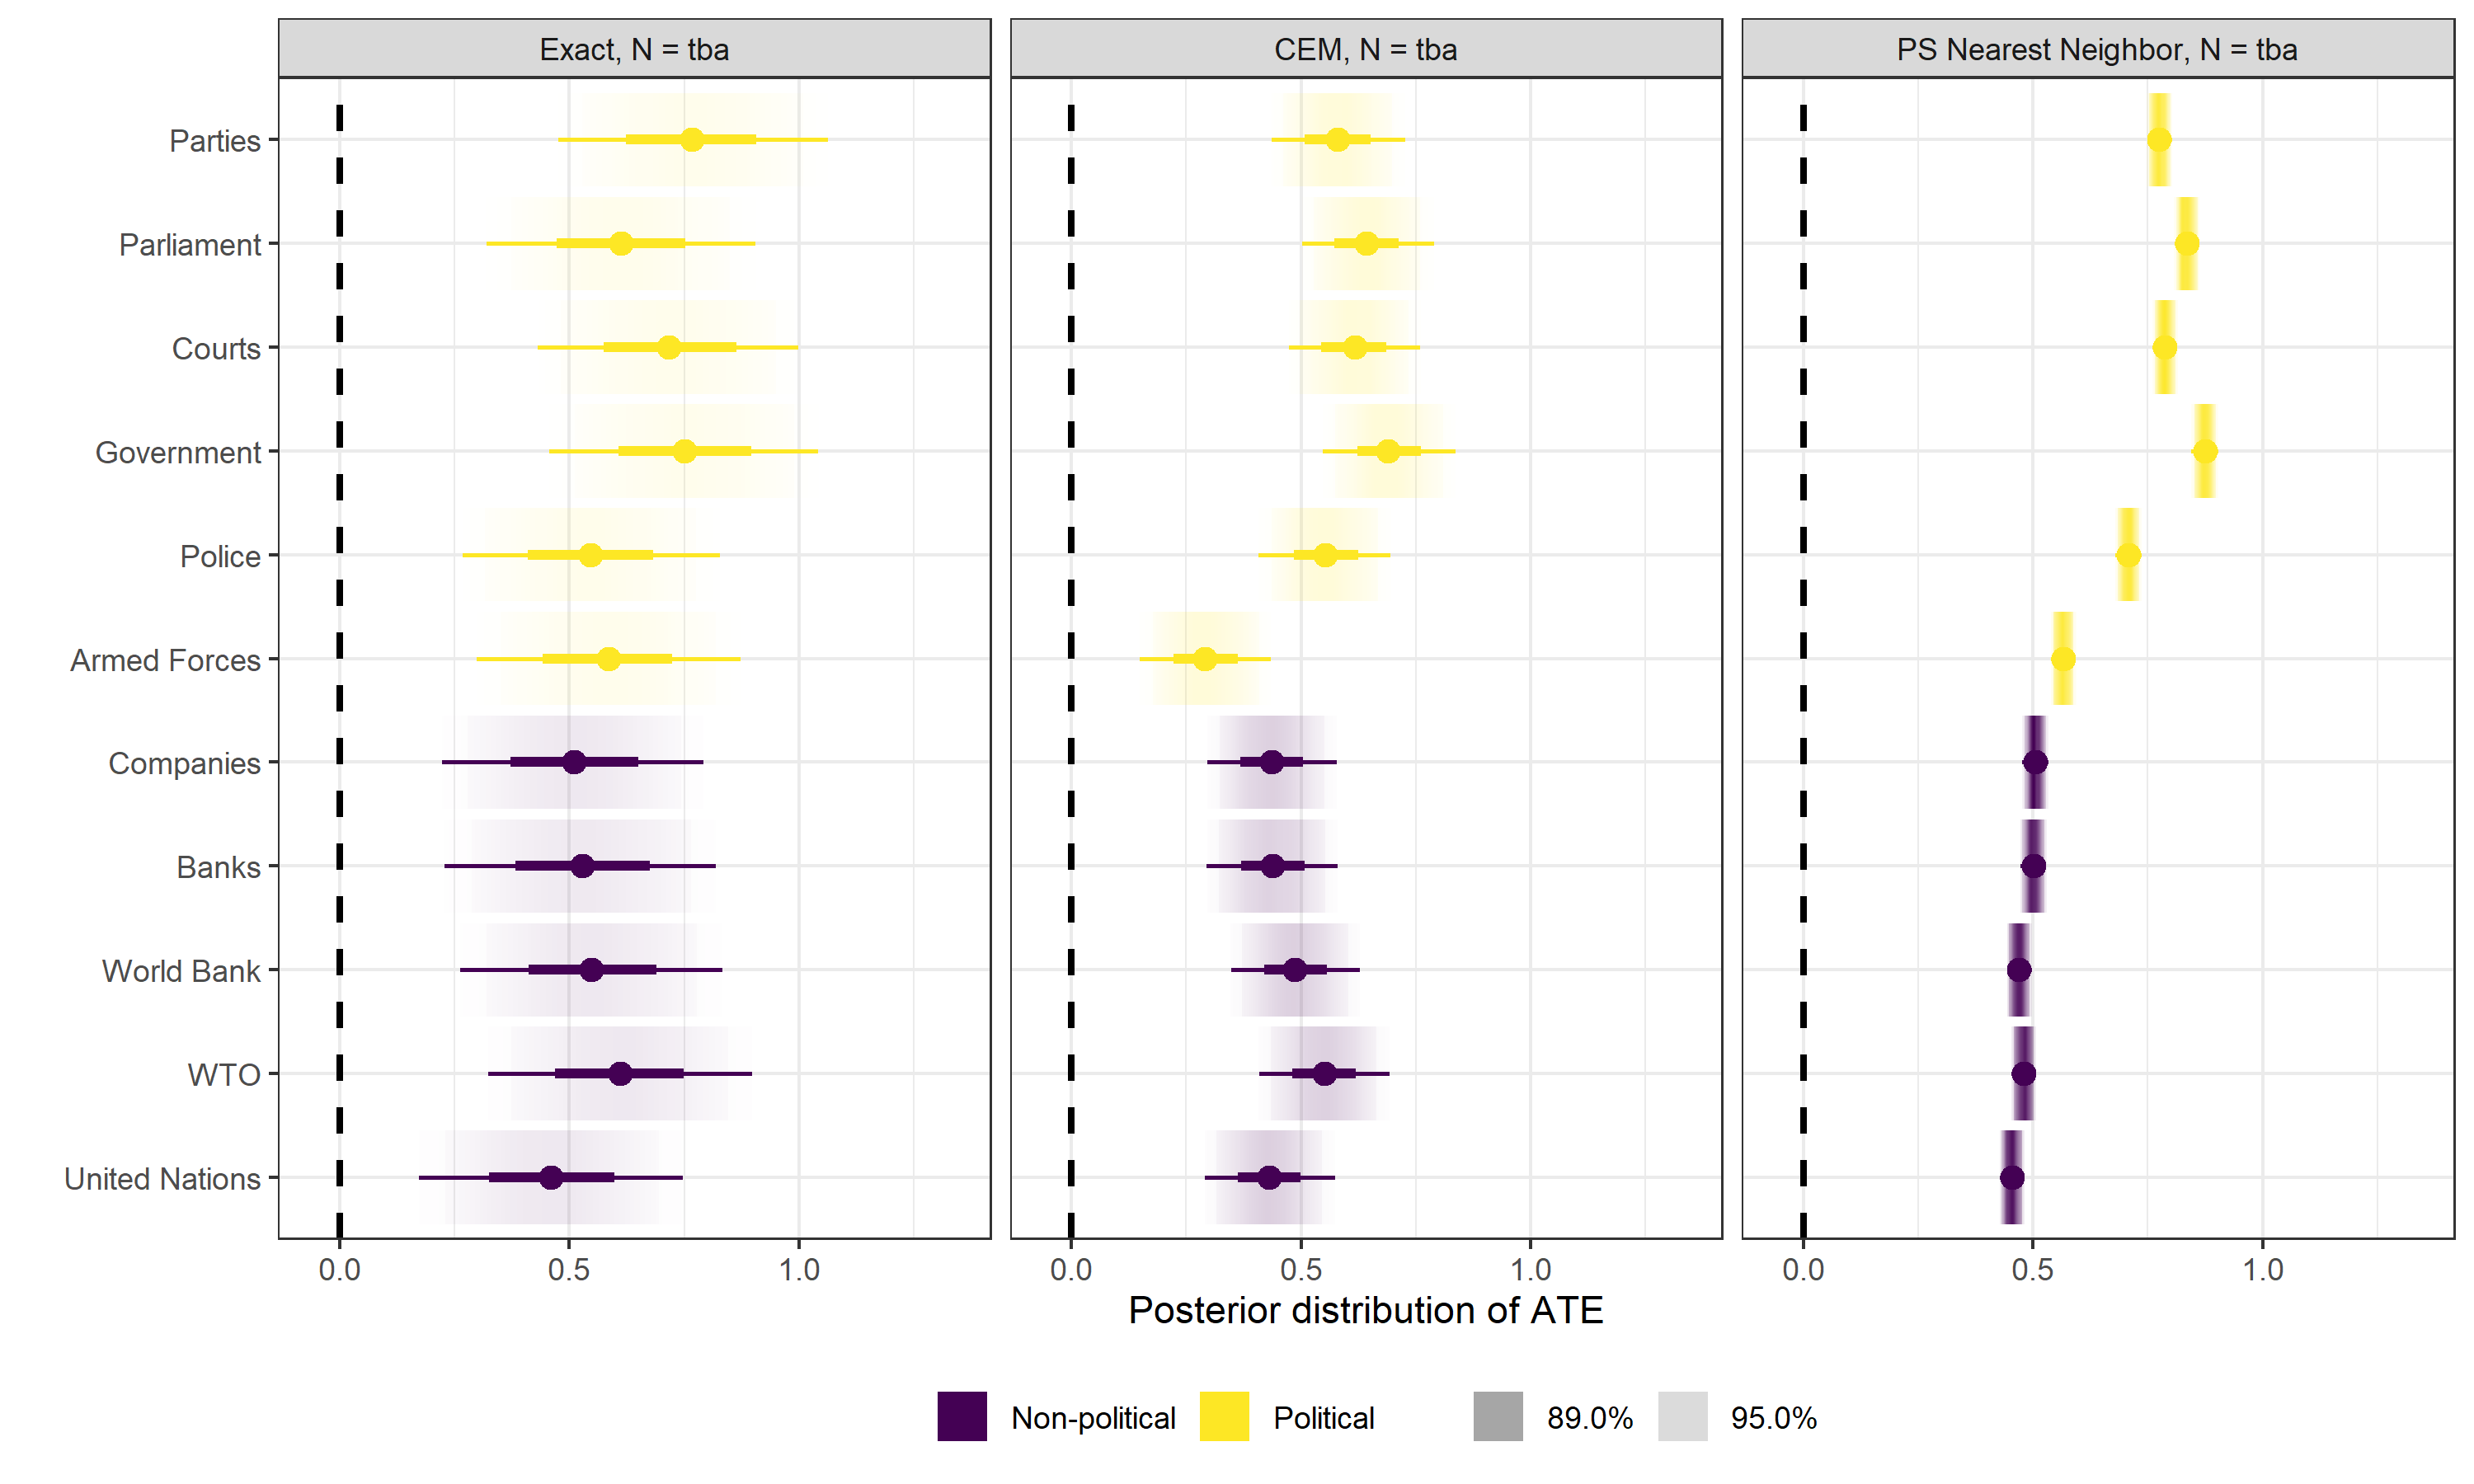
\includegraphics[width=\linewidth,trim=4 4 4 4,clip]{figs/matching.png}\\
	\caption{Average Treatment Effects of Election Integrity Perception on Trust in Institutions from Matching Analysis on WVS Wave 7 (2017-2020) data. Point estimates are means, with 89\% and 95\% confidence intervals depicted with point-ranges and full posterior distributions with the gradient intervals.} 
	\label{fig:matching}
	% \footnotesize{Note: }
\end{figure}

Figure \ref{fig:matching} presents the average treatment effect of the variable of interest, fraud perceptions, from the ordered logit regressions on three matched datasets. Across specifications, we find robust support for our main hypothesis of attitudinal spillover. Perceived prevalence of election day ballot fraud in the federal elections of one's country shows to robustly decrease confidence in political institutions that are unrelated to electoral administration. Yet while trust in institutions related to political sphere seem to be affected by election fraud perceptions, we also observe similar effects of fraud information for non-political institutions, contrary to our expectations. While this pattern may likely be explained by the observational nature of our data, this may still raise concerns regarding the findings for political institutions. Therefore, this discrepancy motivates our core analysis, the survey experiment, which we describe in detail in the following sections. 



\newpage
\section*{Survey Experiment Design}

 
We test our arguments on (i) the attitudinal spillover of election fraud information and (ii) the moderating role of punishments using data from a pre-registered\footnote{The experimental design and all hypotheses have been pre-registered using the Open Science Framework. The pre-registration plan can be accessed via \url{https://osf.io/jyc2n/} (Last accessed June 21, 2022).} online survey experiment that was conducted in Colombia, Mexico, and Russia in April-June of 2021. We first discuss the case selection for the experimental part of our study, then outline the sampling process and provide an overview for the questionnaire. Lastly, we elaborate on the the causal identification strategy.\footnote{Further details of research design can be found in appendix.}


\subsection*{Case Selection}

Focusing on the countries of Colombia, Mexico, and Russia has the advantage of them, on the one hand, sharing a variety of features relevant for our experimental design. In particular, with all three cases, we study middle-income countries with party systems that have shown a sizable degree of stability throughout past decades. These countries also share a large history of public controversies around electoral fraud. On the other hand, these countries are sufficiently different from one another to observe if the mechanisms that we outline travel to diverse political and cultural contexts. 

In the post-World War II era, Mexico underwent a gradual and often described as pendular democratization process (\citealt{Cantu2015}; \citealt{Hiskey2005}). Since the end of the Mexican Revolution in 1917, elections were held regularly in six-year intervals and political opposition was granted passive voting rights. Yet the authoritarian rule of the Institutional Revolutionary Party (PRI) effectively consolidated a hegemonic one-party party system (\citealt{Sartori1976}).
% with only few local opposition parties far from national influence existing parallel to the official administration.
Popular distrust in the legitimacy of Mexican elections roots in the experience of PRI's one-party rule, which was notoriously engaged in attempts of electoral manipulation against parties from both sides of the political spectrum. 
PRI's strategies in balancing out authoritarianism with competitive elections manifested in unrecognized victories of the right-wing National Action Party (PAN) in a multitude of subnational elections in the 1980s and 1990s (\citealt{Greene2007}; \citealt{Cantu2015}), systematic repression against the left-winged Democratic Revolution Party's (PRD) candidates (\citealt{Greene2007}), and election-day fraud such as the manual alteration of vote tallies in multiple regional and national-level contests (c.f. \citealt{Cantu2019b}).
Only after 1980s that electoral contests have become more inclusive and opposition victories occurred and were recognized in state- and local-level elections.
% It was not before the 1980s that electoral competition led to more inclusive electoral contests which produced changing majorities. First, recognized opposition victories occurred in state-level and local elections and only recently culminated in the first national-level contest since the Mexican Revolution of 1920 being decided in favor of the political challenger when the  National Action Party's (PAN) candidate defeated PRI's Francisco Labastida in July 2000. 
Today, Mexico's political party system shows a remarkable level of institutionalization when compared to other new democracies and locates the country on the upper end on the scale of party system stability in Latin America (\citealt{Greene2018}). Notably, the historical baggage of electoral maladministration and attempts of manipulation persists and reaches forward up until the country's most recent electoral events (\citealt{Cantu2014}; \citealt{Cantu2019a}). 

Colombia's history of democratization holds several paradoxes. Formally, regular multi-party elections are held since 1830's, the state claims that it alone can exercise legitimate use of force and the constitution explicitly fosters opposition rights in the political sphere. In practice, electoral events consistently trigger fraud accusations both from the citizenry and academic literature (\citealt{DuqueDaza2019}) and candidates, politicians and journalists are regularly assassinated (\citealt{Bejarano2005}). These and other observations have led scholars of the Colombian case to describe the country as a `besieged' (\citealt{Bejarano2005}) or `fraudulent' electoral democracy (\citealt{DuqueDaza2019}), in which the institutional design and democratic practice of the country diverge strongly, which resembles Mexican case to a large extent. Coupled with cultural similarities, this is the main ground for us treating these two countries as a single Latin American sample of electoral democracies. 

In Russia, we study a context of institutionalized authoritarian rule. After the dissolution of the Soviet Union in 1991, meaningful opposition has effectively been banned since the beginning of Vladimir Putin's administration in 1999 and several observers note that election-day fraud has metasized since in the earlier 2000s (\citealt{Myagkov2009}). Consistently accompanied by widespread fraud allegations, Russian elections are also occasionally followed by anti-regime protests (\citealt{Robertson2017, Lankina2020}). 
% the Russian Duma elections of 2011 in which considerable protests of up to about 150,000 participants were witnessed in Moscow, St. Petersburg and regional capitals (\citealt{Robertson2017}). 
Election monitors routinely condemn Russian elections and a whole range of scholarly contributions focuses on highly unusual patterns in published voting returns that are hard to explain with processes other than manual alteration of vote counts (\citealt{Rozenas2017}; \citealt{Klimek2012}; \citealt{Myagkov2009}; \citealt{Jimenez2017}; \citealt{Kobak2016a, Kobak2016b, Kobak2018}). Studies suggest that in the 2011 parliamentary elections, the vote share of the incumbent United Russia party was at least 11 percentage points lower than documented by official figures (\citealt{Enikolopov2013}). Today, only about 15.5\% of Mexicans, 20.5\% of Colombians, and about 39.8\% of Russians say that election officials are fair and that votes are counted free and fairly.\footnote{Source: World Values Survey Wave 7 (\citealt{Inglehart2020}), 2017-2021.}

Additionally, from the practical point of view, all three countries held or were scheduled to hold federal elections further in 2021, July in Mexico and September in Russia, or May 2022 in Columbia, providing a temporally-comparable political environment for the examination of the electoral misconduct. While in no way exhaustive for a cross-country comparison, this combination of cases still allows us to draw some comparisons across institutional contexts with regards to our findings. 

%%% I still feel like this subsection lacks structure. I wish all of the main reasons were in one or two paragraphs together and there are some issues with cohesion in the background paragraphs... 

\subsection*{Survey Design and Implementation}
% discuss the sample and its non-representativeness
The survey was set up via the online platform \textit{SoSci Survey}, while the respondents from all three countries were recruited using the crowd-sourcing platform \textit{Yandex.Toloka}.\footnote{
	While initially, as stated in the pre-analysis plan, we intended to use a better-known \textit{Amazon Mechanical Turk} for recruiting participants from Latin American countries, the number of workers from the region on that platform was insufficient, which resulted in a compelled deviation from the registered plan. 
	With \textit{Yandex} being a Russian-based company, the recruitment of Russian-speaking respondents there would have been preferable.} 
This approach to data collection comes with the issue of not all societal groups being (equally) represented on the crowd-sourcing platforms (e.g., \citealt{Bartneck2015}; \citealt{Berinsky2012}). 
Our survey was thus predominantly conducted among urban Internet users who are somewhat younger than the general population and have obtained some level of higher education (\citealt{Berinsky2012}). 
The attitudes towards incumbents and political authorities are divided enough among this group (\citealt{Robertson2017}) for us to be able to test both hypotheses. 
Yet most importantly, the socio-demographic profile of our survey respondents specifically targets those population groups that are particularly important for political dynamics such as gathering and sharing sensitive regime information and boosting their publicity by carrying them to the streets in protests.
This makes the adopted sampling strategy rather advantageous over nationally representative surveys for this particular study. 

% In fact, the adopted sampling strategy provides some several advantages over nationally representative surveys for this particular study. 
% First, the demographic groups that we are likely to sample show higher awareness of election monitoring groups (\citealt{Robertson2017}). % is this still a relevant thing to bring up? adjust or delete?
% This assures that respondents give valid answers and, through their background knowledge, can accurately assess the meaning and implications of our treatments. 
% A considerable number of studies have evaluated the use of crowd-sourcing marketplaces for social science research (\citealt{Bartneck2015}; \citealt{Berinsky2012}).
% In line with previous studies investigating demographic predictors of participation in manual crowd-sourced labor, we can confidently assume that 
% The survey was designed to take about ten minutes to complete and started off with a range of socio-demographic identifiers and several questions on political attitudes that are relevant to our expectations. Subsequently, respondents were randomly assigned to treatment and control groups. 
% Regarding respondents in Russia, recent surveys on educated, urban, internet-using citizens have shown that even among these demographic strata, which are often thought to hold views that are particularly opposed to the regime, attitudes towards incumbents and political authorities are very much divided. This makes us confident that we will cover both regime supporters and opponents in our online data collection (\citealt{Robertson2017}).

In addition, while the specific attitudes of these surveyed groups might not be representative of the population as a whole, there is a wealth of evidence amassing that the factors which shape these attitudes are. Research has shown that treatment effects within attitudinal research based on data collected using \textit{Amazon MTurk} are similar to those found in representative surveys (\citealt{Clifford2015}; \citealt{Coppock2019}).\footnote{Similar conclusions have been reached independently from each other across a variety of disciplines (\citealt{Bartneck2015}; \citealt{Yang2015}).} Hence, while our sampled group differs from the general population in terms of their attitudes descriptively, we might well expect the general patterns around their reactions to the experimental stimuli to hold in the general population. 

The survey was designed to take about ten minutes to complete and started off with a range of questions on political attitudes, political knowledge, party affiliation, and general trust.\footnote{Questionnaires as well as privacy and ethical statements are available in appendix.} 
Next, the respondents were randomly assigned to one of four experimental conditions, i.e. they were required to read a paragraph of text related to a hypothetical election. 
Participants were also asked summarize the text upon reading it, which provided us with an attention check and allowed for certain robustness checks.  
Lastly, respondents' trust in institutions was assessed, and the socio-demographic information questions concluded the questionnaire as the final step.
Participants were presented with the survey in either Russian or Spanish. For the questions present in the WVS, such as those on political attitudes and socio-demographics, we have used the validated country-specific translations available in WVS questionnaires. 
For the original questions, the translations were validated through the cognitive interviews with the native speakers. 


\subsection*{Causal Identification}

The experimental design is centered around levels of diffuse support towards the elements of political system and exposes respondents to one of four experimental groups. 
After answering the introductory questions of the survey, respondents are randomly assigned to one of the text fragments described in table \ref{tab:treatments}. 
The text of the first group is neutral and states some basic facts about a hypothetically upcoming election to elect the country's national legislative body, and the respondents are presented with a status quo outcome. 
The second text contains the general information about the election scenario identical to that of the first group, but additionally explicitly exposes respondents to information about malpractices that were allegedly performed on election day omitting the source of the allegations.
% In order to separate the effects of information from the source credibility, we follow the approach in \citet{Reuter2019} with omittig the
% It details accusations of a group of domestic and international observation missions and follows experimental setups such as those to be found in \citet{Bush2018}, \citet{Williamson2021} and \citet{Robertson2017} who also used evaluations of election observer missions as credible measures for fraud information. 
The information presented to the third and fourth groups goes beyond the presentation of general facts about the hypothetical election as well as the description of fraud allegations and exposes respondents to information about punishments from within the political system directed at those individuals who are allegedly responsible for electoral crimes. 
For the third group, the punishment is limited to the actions being undertaken by the superior electoral commission, i.e. the alleged perpetrators lose their positions at the commission. 
For the fourth group, the punishment includes legal actions in which alleged perpetrators were legally convicted for the performance of electoral crimes as well as personal consequences within electoral commissions for which the alleged perpetrators have worked. 
That is, both third and fourth groups receive the information that validates the accusation of fraud from the part of the state but only the fourth group observes explicit intervention of another institution of the regime, i.e. legal action, which may be critical for the occurrence of spill-over effects.  

In order to ensure that exactly one fourth of all respondents per country are placed in each of the four experimental groups and to avoid sparse data problems that might arise from extreme scenarios under complete randomization, we apply a randomized block design separately for each of the countries.
Additionally, to be able to compare the results across regime supporters and opponents, we randomize treatments within these groups. 
% We also include a question asking to summarize the main information from the treatment in a sentence to ensure that the respondents have read the text.    
After being confronted with treatment conditions, respondents are presented with a battery of questions measuring their levels of diffuse support for individual institutions of their political system. 
The most prominent empirical conceptualization of \citet{Easton1975}'s classical concept of diffuse support is political trust (\citealt{Hooghe2012}; \citealt{Schneider2017}; \citealt{Frye2019}). 
Specifically, we ask each participant the following question: \textit{“Upon receiving this information, how much confidence would you have in the following organizations or institutions?”}. 
The battery of items includes \textit{“(1) the armed forces, (2) the police, (3) the justice system/courts, (4) the central electoral commission, (5) the government, (6) the parliament and (7) political parties"} in the random order. 
Following WVS, responses are collected on a four-point scale ranging from “none at all” to “a great deal”. 
Similarly, we include the list of randomly-ordered non-political institutions to validate the limitations of the spillover effects to political institutions. 


\singlespacing
\begin{table}[H]
	\caption{Experimental Treatments.}
	\label{tab:treatments}
	
	\hrule 
	\vspace{0.5cm}
	\textbf{(1) Control group: Neutral information} \\
	On Sunday, \textit{[6 June 2021/19 September 2021/13 March 2022]}, legislative elections are scheduled to be held in \textit{[Mexico/Russia/Colombia]}. 
	More than [2,000/2,000/1,000] registered candidates will compete for the \textit{[500/450/280]} parliamentary seats of the \textit{[Champer of Deputies/State Duma/Congress of Colombia]}. 
	The results will be determined by nearly \textit{[90/110/36]} million \textit{[Mexicans/Russians/Colombians]}.
	Imagine that the elections have already passed and suppose that as in the current convocation, \textit{eight/four/twenty} parties retained seats in the assembly. \\
	
	\textbf{(2) Treatment group: Fraud information} \\
	\hl{$[$Neutral information$]$} \\
	In this hypothetical scenario, suppose that after election day, it becomes known that ballot-box stuffing and alterations of vote tallies in favor of the incumbent party perpetrated by individuals working for electoral commissions were widespread. 
	Suppose that these electoral misconducts and manipulation practices took place across several regions of the country. \\
	
	% On an after election day, however, allegations of ballot-box stuffing and alterations of vote tallies perpetrated by individuals working for electoral commissions in favor of the incumbent party were widespread. Shortly after election day, a number of domestic and international election observation missions publicly called out a variety of electoral misconducts and manipulation practices across several regions of the country. \\
	
	\textbf{(3) Treatment group: Fraud information with electoral commission punishment} \\ 
	\hl{$[$Neutral information$]$} \\
	\hl{$[$Fraud information$]$} \\
	Furthermore, suppose that as a consequence, individuals allegedly responsible for fraud lost their position in the electoral commissions that they served in.\\
	
	\textbf{(4) Treatment group: Fraud information with court and electoral commission punishment} \\
	\hl{$[$Neutral information$]$} \\
	\hl{$[$Fraud information$]$} \\
	Furthermore, suppose that as a consequence, individuals allegedly responsible for fraud lost their position in the electoral commissions that they served in. 
	Also, legal action was brought against these individuals, who were convicted for electoral crimes by responsible courts.
	\vspace{0.5cm}
	\hrule
\end{table}
\doublespacing

% The neutral statement reflects the status quo rather than explicitly specifying the absence of any fraud. Such a statement allows us to compare the effects of explicit discussion of fraud to the pre-existing beliefs of respondents about the political system. We would hence expect smaller differences for the opponents of the regime, who are likely to already presume a certain degree of fraud of some kind. 

A range of important characteristics of the experimental design can be noted in relation to the spillover theory outlined above.
First, the text fragments that are presented to members of the treatment groups explicitly discuss the \textit{mechanisms} of alleged election-day\footnote{To be precise, the elections in Russia were in fact conducted within three days rather than one, September 17-19, with addition of other features like electronic voting, yet these decisions had not been officially finalized by the Central Electoral Commission by the start of the survey, and thus were not depicted in the treatment text.} fraud. 
This should allow us to avoid variations in the interpretations of our fraud treatment, for instance associations of vote buying in Mexico (\citealt{Cantu2019a}), and hence prevent heterogeneous effects related to this vagueness. 
% and ballot box stuffing in Russia (\citealt{Myagkov2009}). 
Second, referring to `individuals working for electoral commissions', we explicitly state the alleged \textit{perpetrator of fraud}. 
Mentioning the perpetrator is crucial as it allows us to directly study if trust is extrapolated to different bodies that are unrelated to administration of elections. 

Importantly, not all of the institutions included in our battery on political trust allow us to unambiguously identify \textit{spillover} effects. 
For example, it is hard to disentangle whether fraud in new democracies or electoral authoritarian regimes constitutes the actions of micro-level agents or whether these practices are instructed from party and/or state representatives. 
For citizens who expect the latter, information about election day fraud may actually function as informational cues implying partisan involvement from political authorities. 
Among these participants, changes in diffuse support for the institutions of the government, parliament, political parties and central electoral commission may not necessarily be the result of an attitudinal spillover following from trust extrapolation as we theorize.
Instead, it can be a straightforward withdrawal of political support from the perceived perpetrator of electoral misconduct. 
While substantively relevant, this scenario would not provide evidence for our outlined theory on information processing, which focuses on the \textit{extrapolation} of trust which spills over to unaffected branches of the political system.

% We use two strategies to counter this possibility. 
To counter this possibility, 
% First, 
we ask for respondents' levels of diffuse support towards a number of institutions that are clearly exogenous to our fraud treatment. 
Without spillover, trust in institutions such as the armed forces, the police, or the justice system are unaffected by information on election day manipulation, as members of these institutions are unrelated to fraudulent interference practiced by individuals working for electoral commissions on voting day. 
In contrast, decays in diffuse support towards these institutions as a response to the fraud treatments present genuine spillover effects. 
% Second, in order to disentangle whether changes in diffuse support for the institutions of the central electoral commissions, government, parliament and political parties represent genuine spillover effects as stated by Hypothesis 1 or merely a direct withdrawal of support from assumed perpetrators, we include a follow-up question after our treatment and the responses to the political trust battery asking: \textit{... some people say that there are systematic irregularities to be observed in the federal elections of [country], while other people deny that. Given that such claims were true, to which extent do you expect representatives of political parties and state-affiliated agents to be involved?”}. 
Changes in diffuse support among those respondents who do not expect party representatives playing a role in fraudulent interference are considerably less prone to treatment endogeneity and hence provide a more realistic estimate of the causal effect even towards institutions that might be implicitly associated with our fraud treatment. 

\newpage
\section*{Analysis and Findings}

\subsection*{Statistical Modeling and Estimation}

To test Hypothesis 1 (the effect of exposure to the information about electoral fraud on confidence in institutions), we estimate the mean difference between the control group (1) and treatment group (2) in table \ref{tab:treatments}, i.e. those individuals who have only received information about the status quo and about fraud explicitly, respectively.
To evaluate Hypotheses 2a and 2b (heterogeneous effects of punishment across supporters and opponents), we estimate the differences between group (2), which only received fraud information, and either group (3) or (4), who received punishment information on top of fraud information. We also allow for varying effects across supporters and opponents constructing a binary variable, based on the pre-treatment party affiliation measure, as a moderator variable. 

% While the random assignment of respondents to treatment and the control groups allows for an unbiased estimate of our treatment effect, we present additional models alongside the raw effects and present adjusted mean differences which take into account a range of socio-demographic information which might influence responses to the outlined fraud treatments and political attitudes such as levels of diffuse support. 
%Since research has provided consistent evidence that perceptions of electoral fairness are divided along partisan lines (c.f. \citealt{Cantu2015}), we include two measures of political support. 
%We ask individuals to which extent they support the current incumbent government and request them to report their partisan identification. 
%Since younger, urban and highly educated individuals have been found to show the highest protest propensities in new democracies and electoral authoritarian regimes, we include measures of age, urbanity and the \textit{ISCED-2011} scale as a measure for education in our models. 
%As we know that individuals' levels of social and political trust are related and individuals' `generalized trust in the world' might well predict their responses to our fraud treatments and their levels of diffuse support, we include a measure of interpersonal trust asking \textit{“Generally speaking, would you say that most people can be trusted or that you need to be very careful in dealing with people?”}. % this is a post-treatment moderator, too, and it may not be the best idea to include it after all... 
%Since private sector workers and individuals employed by the state itself may hold different views towards the political system, we include a dummy indicating private sector workers. 
% Additional controls include measurements for gender, occupational status, household income and individuals' position on the left-right scale.  

Since our dependent variables take on the form of ordered categorical vectors comprising four categories $j$, with $(j = 1,...,4)$, we estimate a set of ordered logistic regressions with following specifications:

\begin{equation}
	% \begin{split}
	\small
	ln \left (\frac{\text{Pr}(y_i \leq j)}{\text{Pr}(y_i > j)} \right) &= \underbrace{\underbrace{\alpha_j - 
		({\beta_1} {\text{ Control}_i} + 
		\beta_2 {\text{ Punishment}_i} + 
		\beta_3 {\text{ Judicial Punishment}_i})
		}_{\text{Main Specification (H1)}} \times 
		\beta_4 \text{ Opponent}_i,}_{
		\text{Heterogeneous Effects Specification (H2)}}
	% \end{split}
\end{equation}

\noindent where $y_i$ is the level of diffuse support of an individual $i$ with ($i=1,...,n$) for an institution, and Control, Punishment, and Judicial Punishment are binary indicators for membership in the experimental groups (2),  (3), and (4) \footnote{Individuals who only received fraud information serve as the reference category in our analysis.}. We analyze Russian and Latin American samples separately, using all available observations that fulfill the basic data-quality criteria, such as completing the questionnaire in lower than 3 minutes, as per the pre-registration plan. 
% $\bm{X}$ is an $i \times k$ vector of covariates ($k=1,...,k$), 
% $\alpha_j$ are threshold parameters, 
% $\bm{\beta}$ are the regression parameters for the covariates 
% and $\beta_1, \beta_2$ are the main parameters of interest.

For parameter estimation, we employ a fully Bayesian framework for statistical inference as implemented in Stan (\citealt{StanDevelopmentTeam2020}). 
Specifically, we rely on Hamiltonian Monte Carlo sampling in which priors are defined to follow Student-$t$ distributions with three degrees of freedom.
% are centered around zero and take on a sufficiently large variance to ensure that priors are uninformative and do not favor any of the substantial hypotheses. 
We run a set of four Markov chains out of which we discard the first 3,500 as warm-up and use the following 2,500 samples to describe posterior distributions, which result into 10,000 post-warmup samples. We check for model convergence using the Gelman-Rubin diagnostic and consider models converged if the discrepancy measure stays below 1.1 (\citealt{Gelman2004}).

%While relying on a Bayesian framework holds general advantages as it allows us to state the uncertainties around our results in straightforward probabilistic statements, it provides very specific advantages to our substantive questions at hand. As our hypotheses on the moderating effect of court rulings evolve around two competing expectations expressed in Hypothesis 2a and 2b, we exploit formal Bayesian hypothesis testing using the Bayes factor defined as 

%\begin{equation}
%    BF_{ab} = \frac{m(H_{2a}|y,\bm{X})}{m(H_{2b}|y,\bm{X})}
%\end{equation}

%\noindent to comparatively quantify to which extent the data favors one hypothesis over the other (\citealt{Kass1995}; \citealt{Gill2015}). For Bayes factor estimation, we rely on the approximate adjusted fractional Bayes factor as developed by \citet{Gu2018} and implemented in the package \texttt{bain} (\citealt{bain2020}) within the R software environment (\citealt{R2020}) that is particularly well suited for the evaluation of competing directional hypotheses. 

\subsection*{Empirical Results}

Due to the nature of the dependent variable, we use ordered logistic regression to evaluate the effects of fraud and punishment information on trust in institutions. To facilitate the substantive interpretation of the estimates, using posterior draws we first calculate individuals' probabilities of selecting each of the four answer categories in evaluating institutional trust. We then calculate the differences in probabilities between those who received fraud information alone and those assigned to another condition - control or one of the punishment conditions. These quantities allow us to compare the effects substantively to our main scenario of interest - exposure to explicit fraud information alone. As a result, the differences for the control and fraud condition serve to evaluate the first hypothesis, while the differences for the two punishment conditions allow for testing of the second one. Given that for one of the punishment conditions another institution of a political system is explicitly mentioned, extrapolation may be more likely to occur there, which is why we treat these conditions separately in the analysis. The former two plots in the section contain the estimates for the full samples for both Russia and Latin America, while the latter two depict the differences in effects across the supporters and opponents. Number of observations per institution varies somewhat as we used all complete data points for each model we estimated. 


% \begin{figure}[H]
%     \centering
%     \caption{The Effect of Exposure to Fraud and Punishment Information on Confidence in Political Institutions in Latin America (pooled sample).}
%     \singlespacing
%     \raggedright
%     \footnotesize{Notes: Positive values on the horizontal axis indicate that the probability of selecting a category is higher in fraud condition than in the other one. Conversely, negative values mean that respondent's probability to choose this was lower in fraud condition. Dashed line schematically depicts the hypothesized relationship between categories, i.e. point estimates would loosely follow the pattern of the dashed line if the relationship between trust and fraud information is as expected. Transparent point ranges include zero in the 89\% highest density interval.}   
%     \label{fig:main-la}
%     % \footnotesize{Note: }
% \end{figure}

\begin{figure}[H]
	\centering
	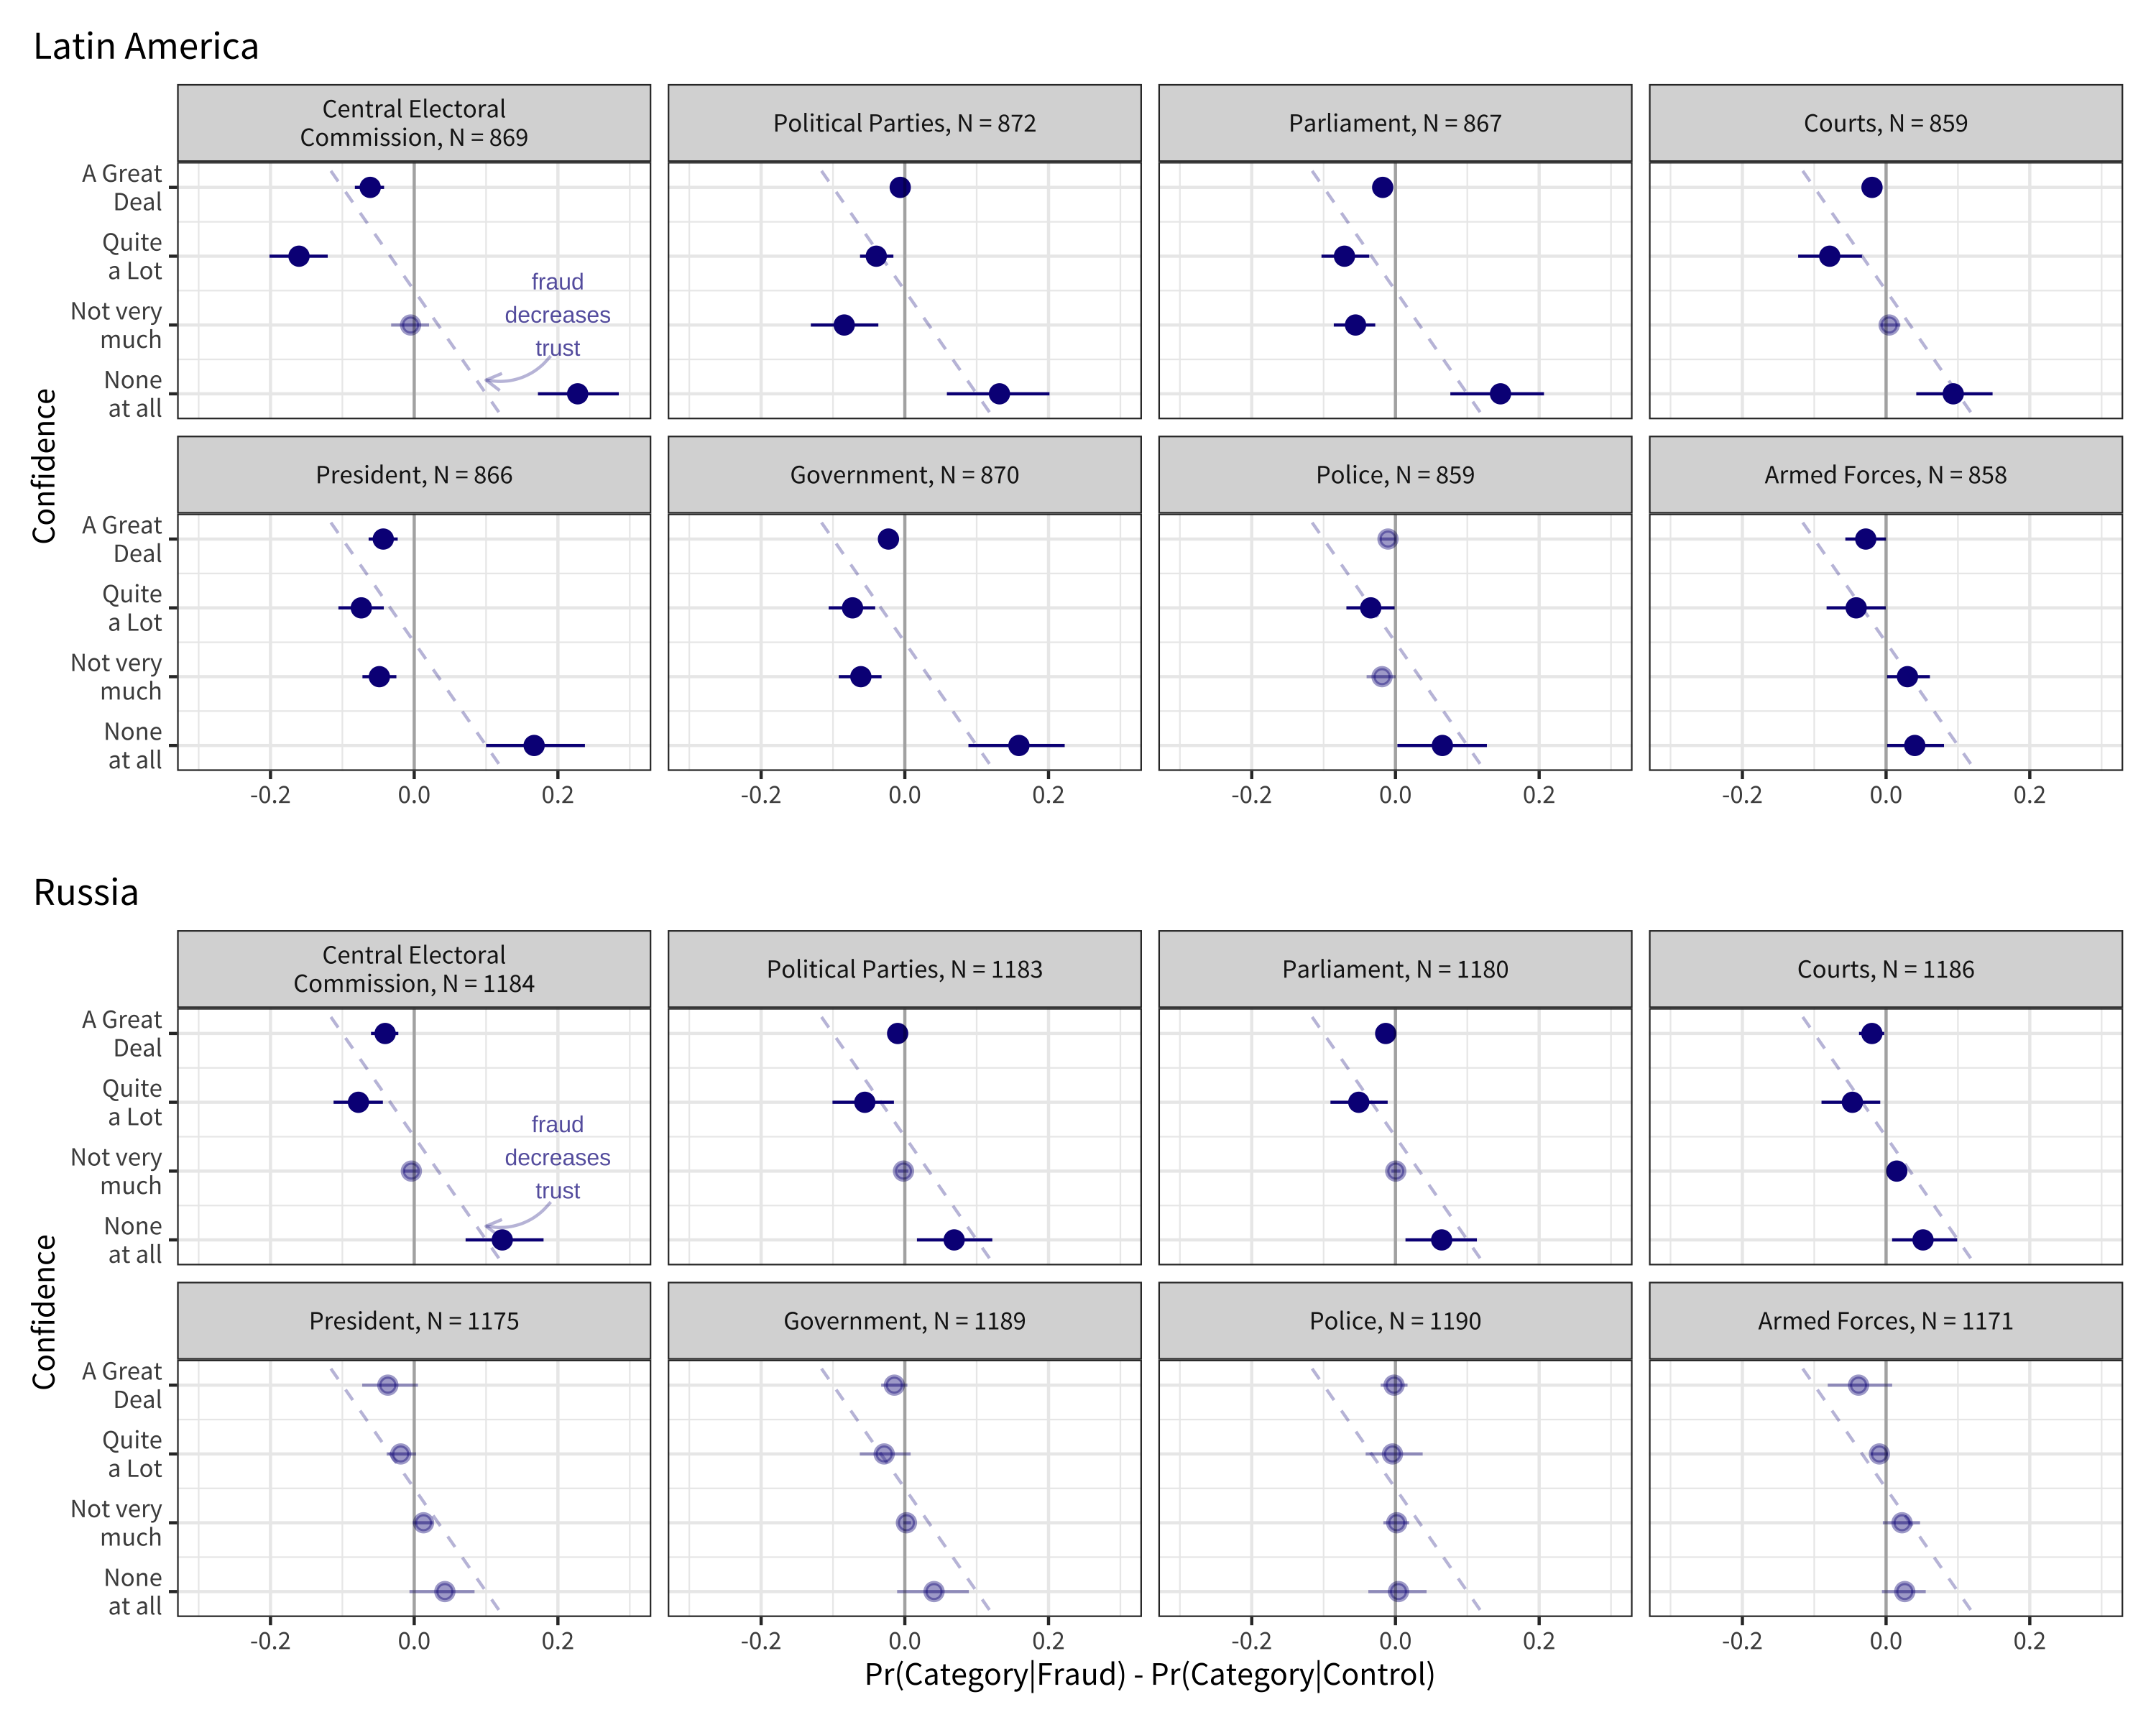
\includegraphics[width=\linewidth,trim=4 4 4 4,clip]{figs/main_hdi89_1.png}
	\caption{The Effects of Exposure to Fraud Information on Confidence in Political Institutions.  \\
		\footnotesize{Notes: Plots depict medians and 89\% highest-density continuous intervals for differences in probabilities for choosing respective categories based on draws from the expectation of the posterior predictive distributions. Probabilities are calculated with ordered logit model estimates.
			%  Positive values on the horizontal axis indicate that the probability of selecting a category is higher in fraud condition than in the other one. Conversely, negative values mean that respondent's probability to choose this was lower in fraud condition. 
			Dashed line schematically depicts the hypothesized relationship between categories, i.e. point estimates would loosely follow the pattern of the dashed line if the relationship between trust and fraud information is as expected. Transparent point ranges include zero in the 89\% HDCI.
	Data were collected in April-June 2021 via an original online survey. } }
	\singlespacing
	\raggedright
	    
	\label{fig:main}
\end{figure}


The results presented in figure \ref{fig:main} in line with the first hypothesis about the effect of fraud information on diffuse support. Across both Russian and Latin American samples, while modest in size, point estimates for the differences between control an fraud conditions are consistent with the expectations. For all institutions, the point estimates for differences are negative for categories indicating higher levels of trust, i.e. the probability of demonstrating more confidence in institutions is higher when being exposed to the control condition than when exposed to the fraud information, and vica versa for the categories for lower trust. While unsurprisingly, the largest differences are present for the central electoral commissions, the differences for many political institutions, both involved in the conduct of elections and not, are significantly different from zero, basing on a 89\% HDCIs, which points toward the presence of spillover effects. We are less likely to observe the spillover effects for police and armed forces for both samples though, which have a less direct relationship to politics per se. Coupled with the lack of spillover effects for non-political institutions (see appendix), this provides evidence for the limits of trust extrapolation and its diminishing with potentially growing perceived distance from the electoral field. 

Notably, the effect sizes are somewhat higher in Latin American sample in comparison to the Russian one, with absolute differences between control and fraud conditions not exceeding 13 percentage points in Russia and 27 percentage points in Latin America. This fact could be related to countries' political regimes and point towards larger discrepancies in the status quo evaluation. The differences would be less pronounced between explicit indication of fraud and the control condition, which could potentially prompt the pre-existing notions of manipulation should respondents have any doubts regarding the presence of fraud in status quo. This provides a harder test for the theory and, coupled with a relatively small sample size, it makes the magnitude of the effects potentially smaller for the entire sample. 

When it comes to the effect of punishment and potential restoring of confidence in institutions in response to observing it or deepening of detrimental effects, the analysis on full samples shows little to no significant difference between fraud and simple punishment scenarios. 
Even further, for the institutions like the armed forces and police in Latin America, mere exclusion from the commission with no further action lowered trust, on average, even further. Splitting between opponents and supporters (figure \ref{fig:het}) indicates that this is largely driven regime supporters' responses, while the opponents' responses are close to the ones in fraud condition. We can observe a similar pattern for trust in courts and CEC in Russia, yet the sample sizes are likely responsible for large uncertainty for these point estimates. While these observations are in line with hypotheses 2, i.e. stronger spillovers among the regime supporters, for other institutions we only observe slight mitigation of the damage or no effect of mere exclusion from the commission on diffuse support in the institutions of political system.

Yet with the addition of legal action in response to fraud, i.e. the judicial punishment condition, the samples differ somewhat in the trends.
In Latin America, only for directly mentioned in the treatment courts and the parliament would we see sizable changes in trust in full samples in the restorative direction, and subgroup analysis reveals that these effects seem to be driven by the opponents' responses, which is in line with the expectations.  
In Russia, these same effects seem to be more pronounced.
In fact, we would see restoring of trust to almost the same level as the control condition and even some gains in trust relative to control condition, meaning that the negative effect of fraud information was overridden completely with an adequate within-system response. We observe these patterns in both full- and subsample analysis (figures \ref{fig:main} and \ref{fig:het} respectively), yet not for the Central Electoral Commission but for other institutions, and among at least either opponents or supporters or often both. 


\begin{figure}
	\centering
	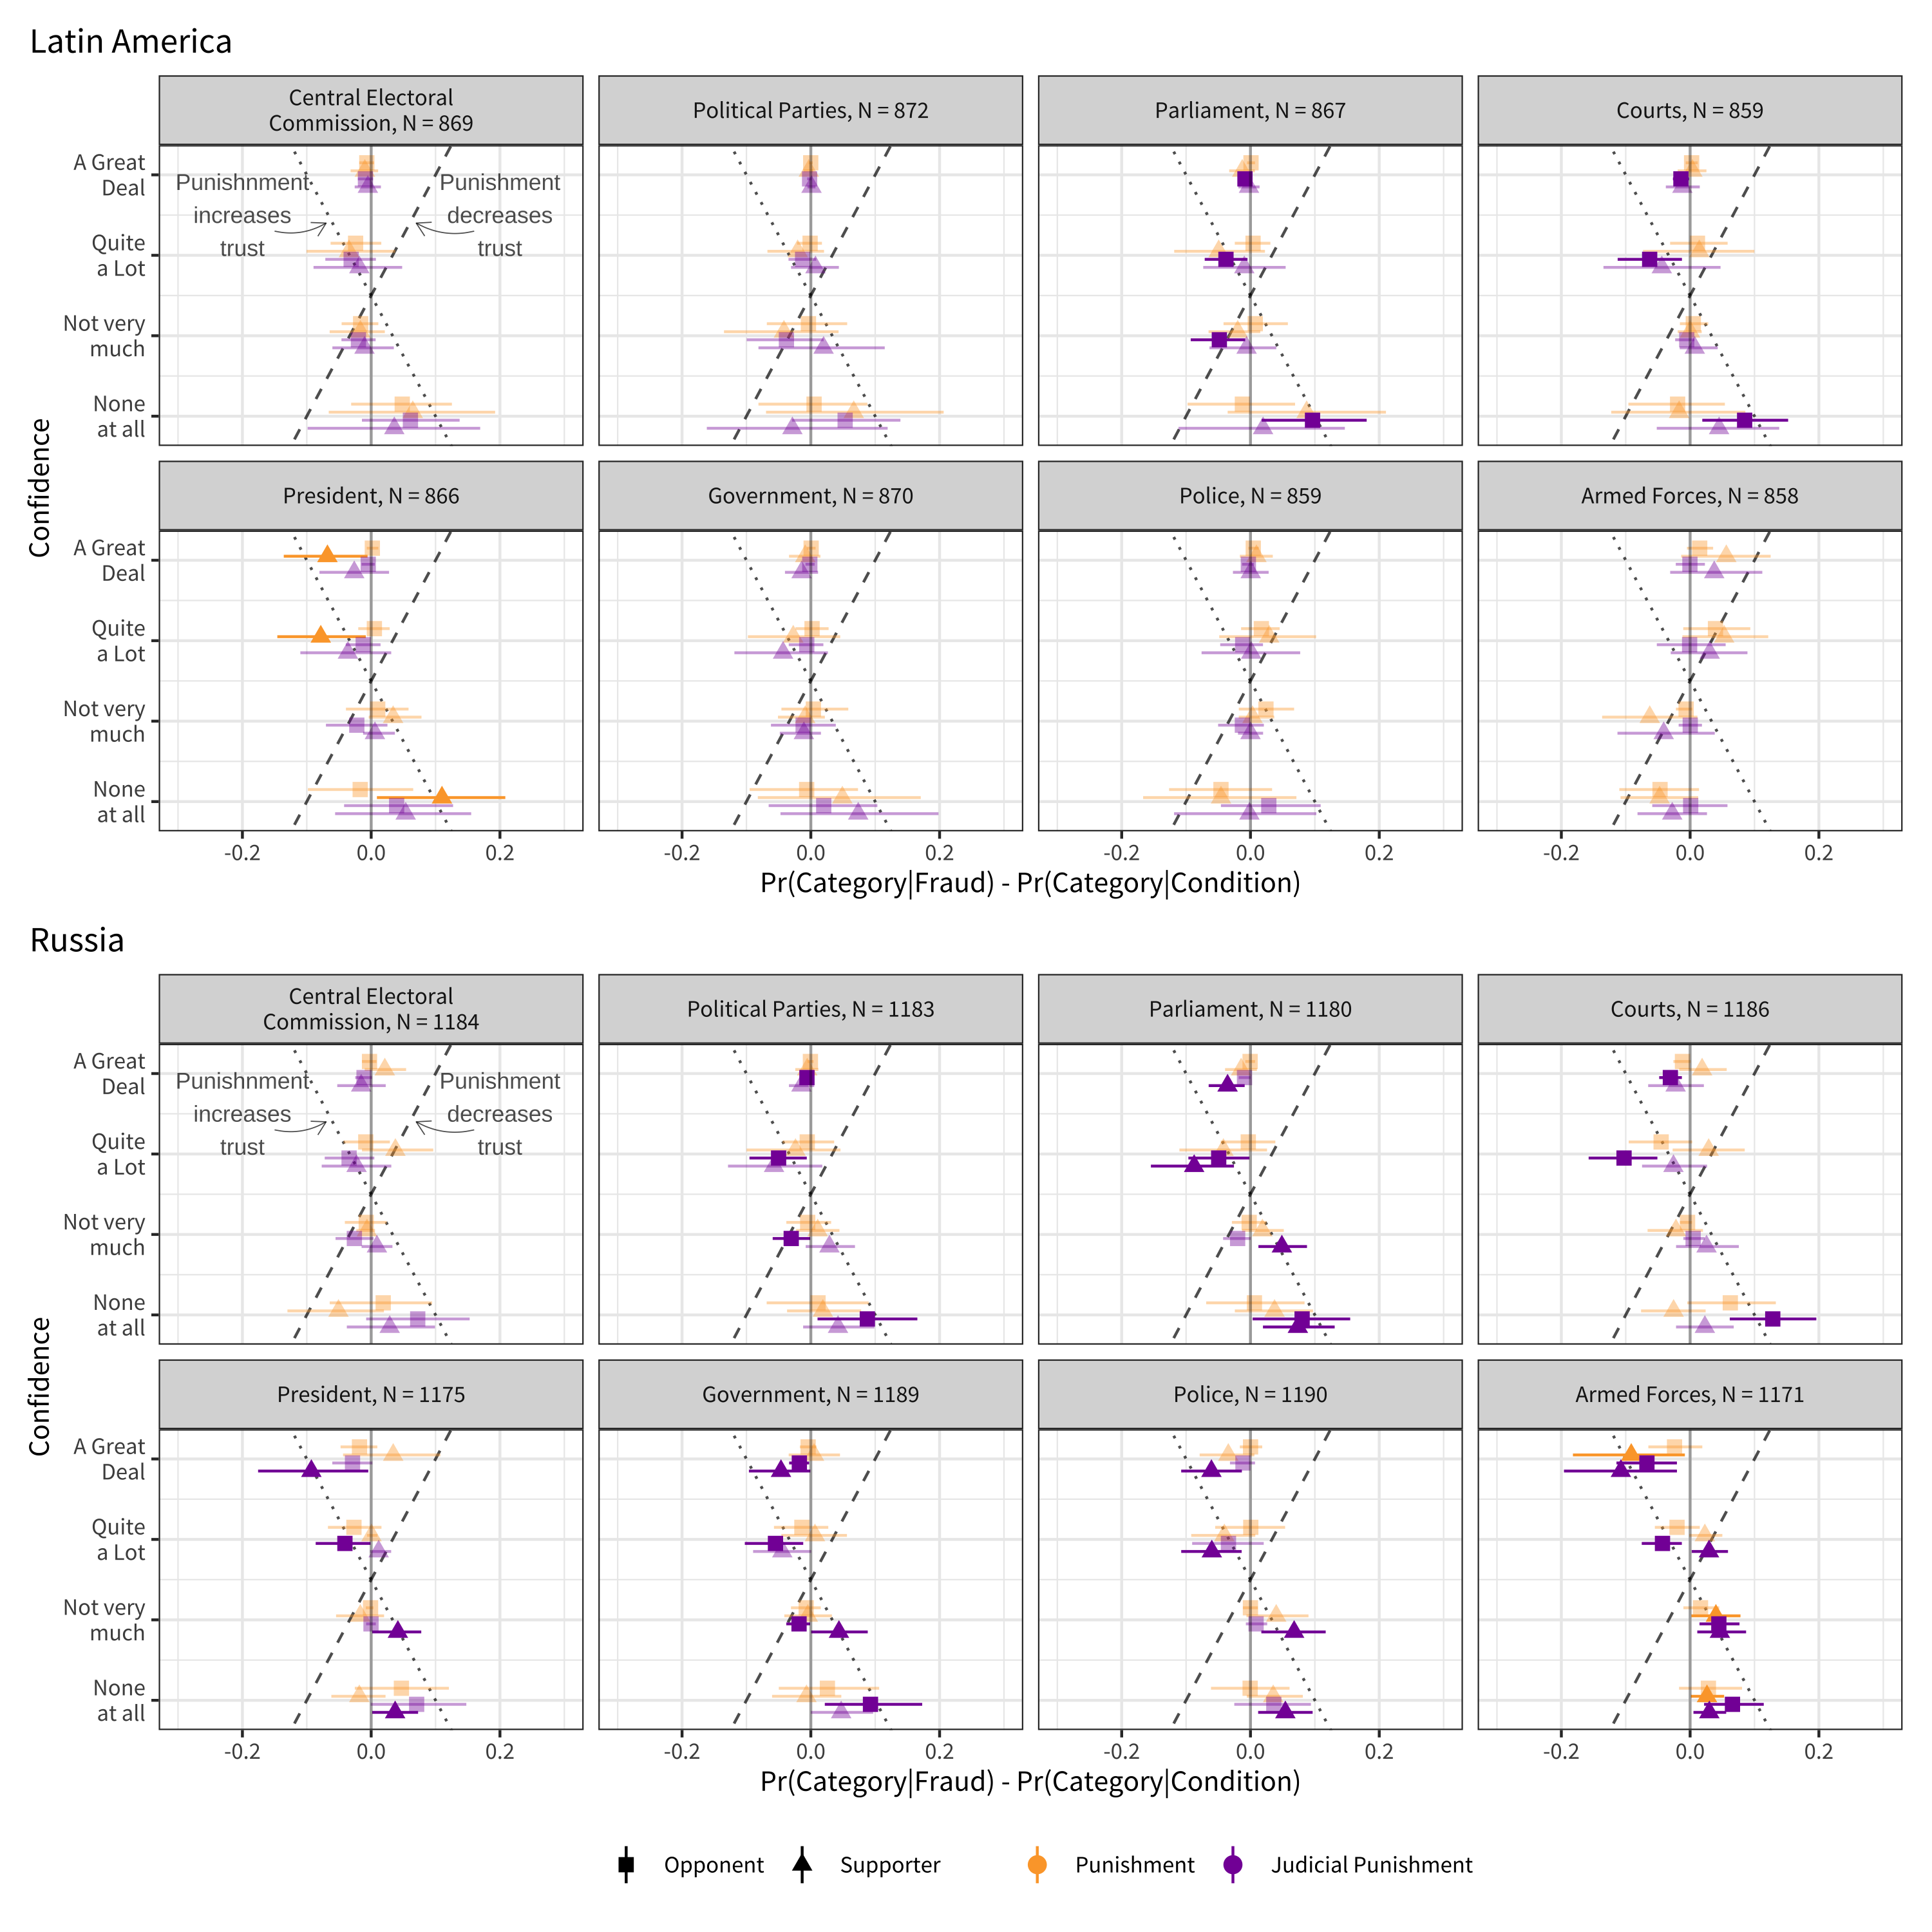
\includegraphics[width=\linewidth,trim=4 4 4 4,clip]{figs/cond_hdi89_1.png}
	% \singlespacing
	% \raggedright
	\caption{The Effects of Exposure to Perpetrators' Punishment Information on Confidence in Political Institutions.  \\
		\footnotesize{Notes: Plots depict medians and 89\% highest-density continuous intervals for differences in probabilities for choosing respective categories based on draws from the expectation of the posterior predictive distributions. Probabilities are calculated with ordered logit model estimates.
			%  Positive values on the horizontal axis indicate that the probability of selecting a category is higher in fraud condition than in the other one. Conversely, negative values mean that respondent's probability to choose this was lower in fraud condition. 
			Dashed (dotted) lines schematically depict the hypothesized relationships between categories, i.e. point estimates would loosely follow the pattern of the dashed (dotted) line if the relationship between trust and within-system response is amplifying (diminishing) the effect of fraud information on trust. Transparent point ranges include zero in the 89\% HDCI.
	Data were collected in April-June 2021 via an original online survey. } }
	\label{fig:het}
\end{figure}

% \begin{figure}
%     \centering
%     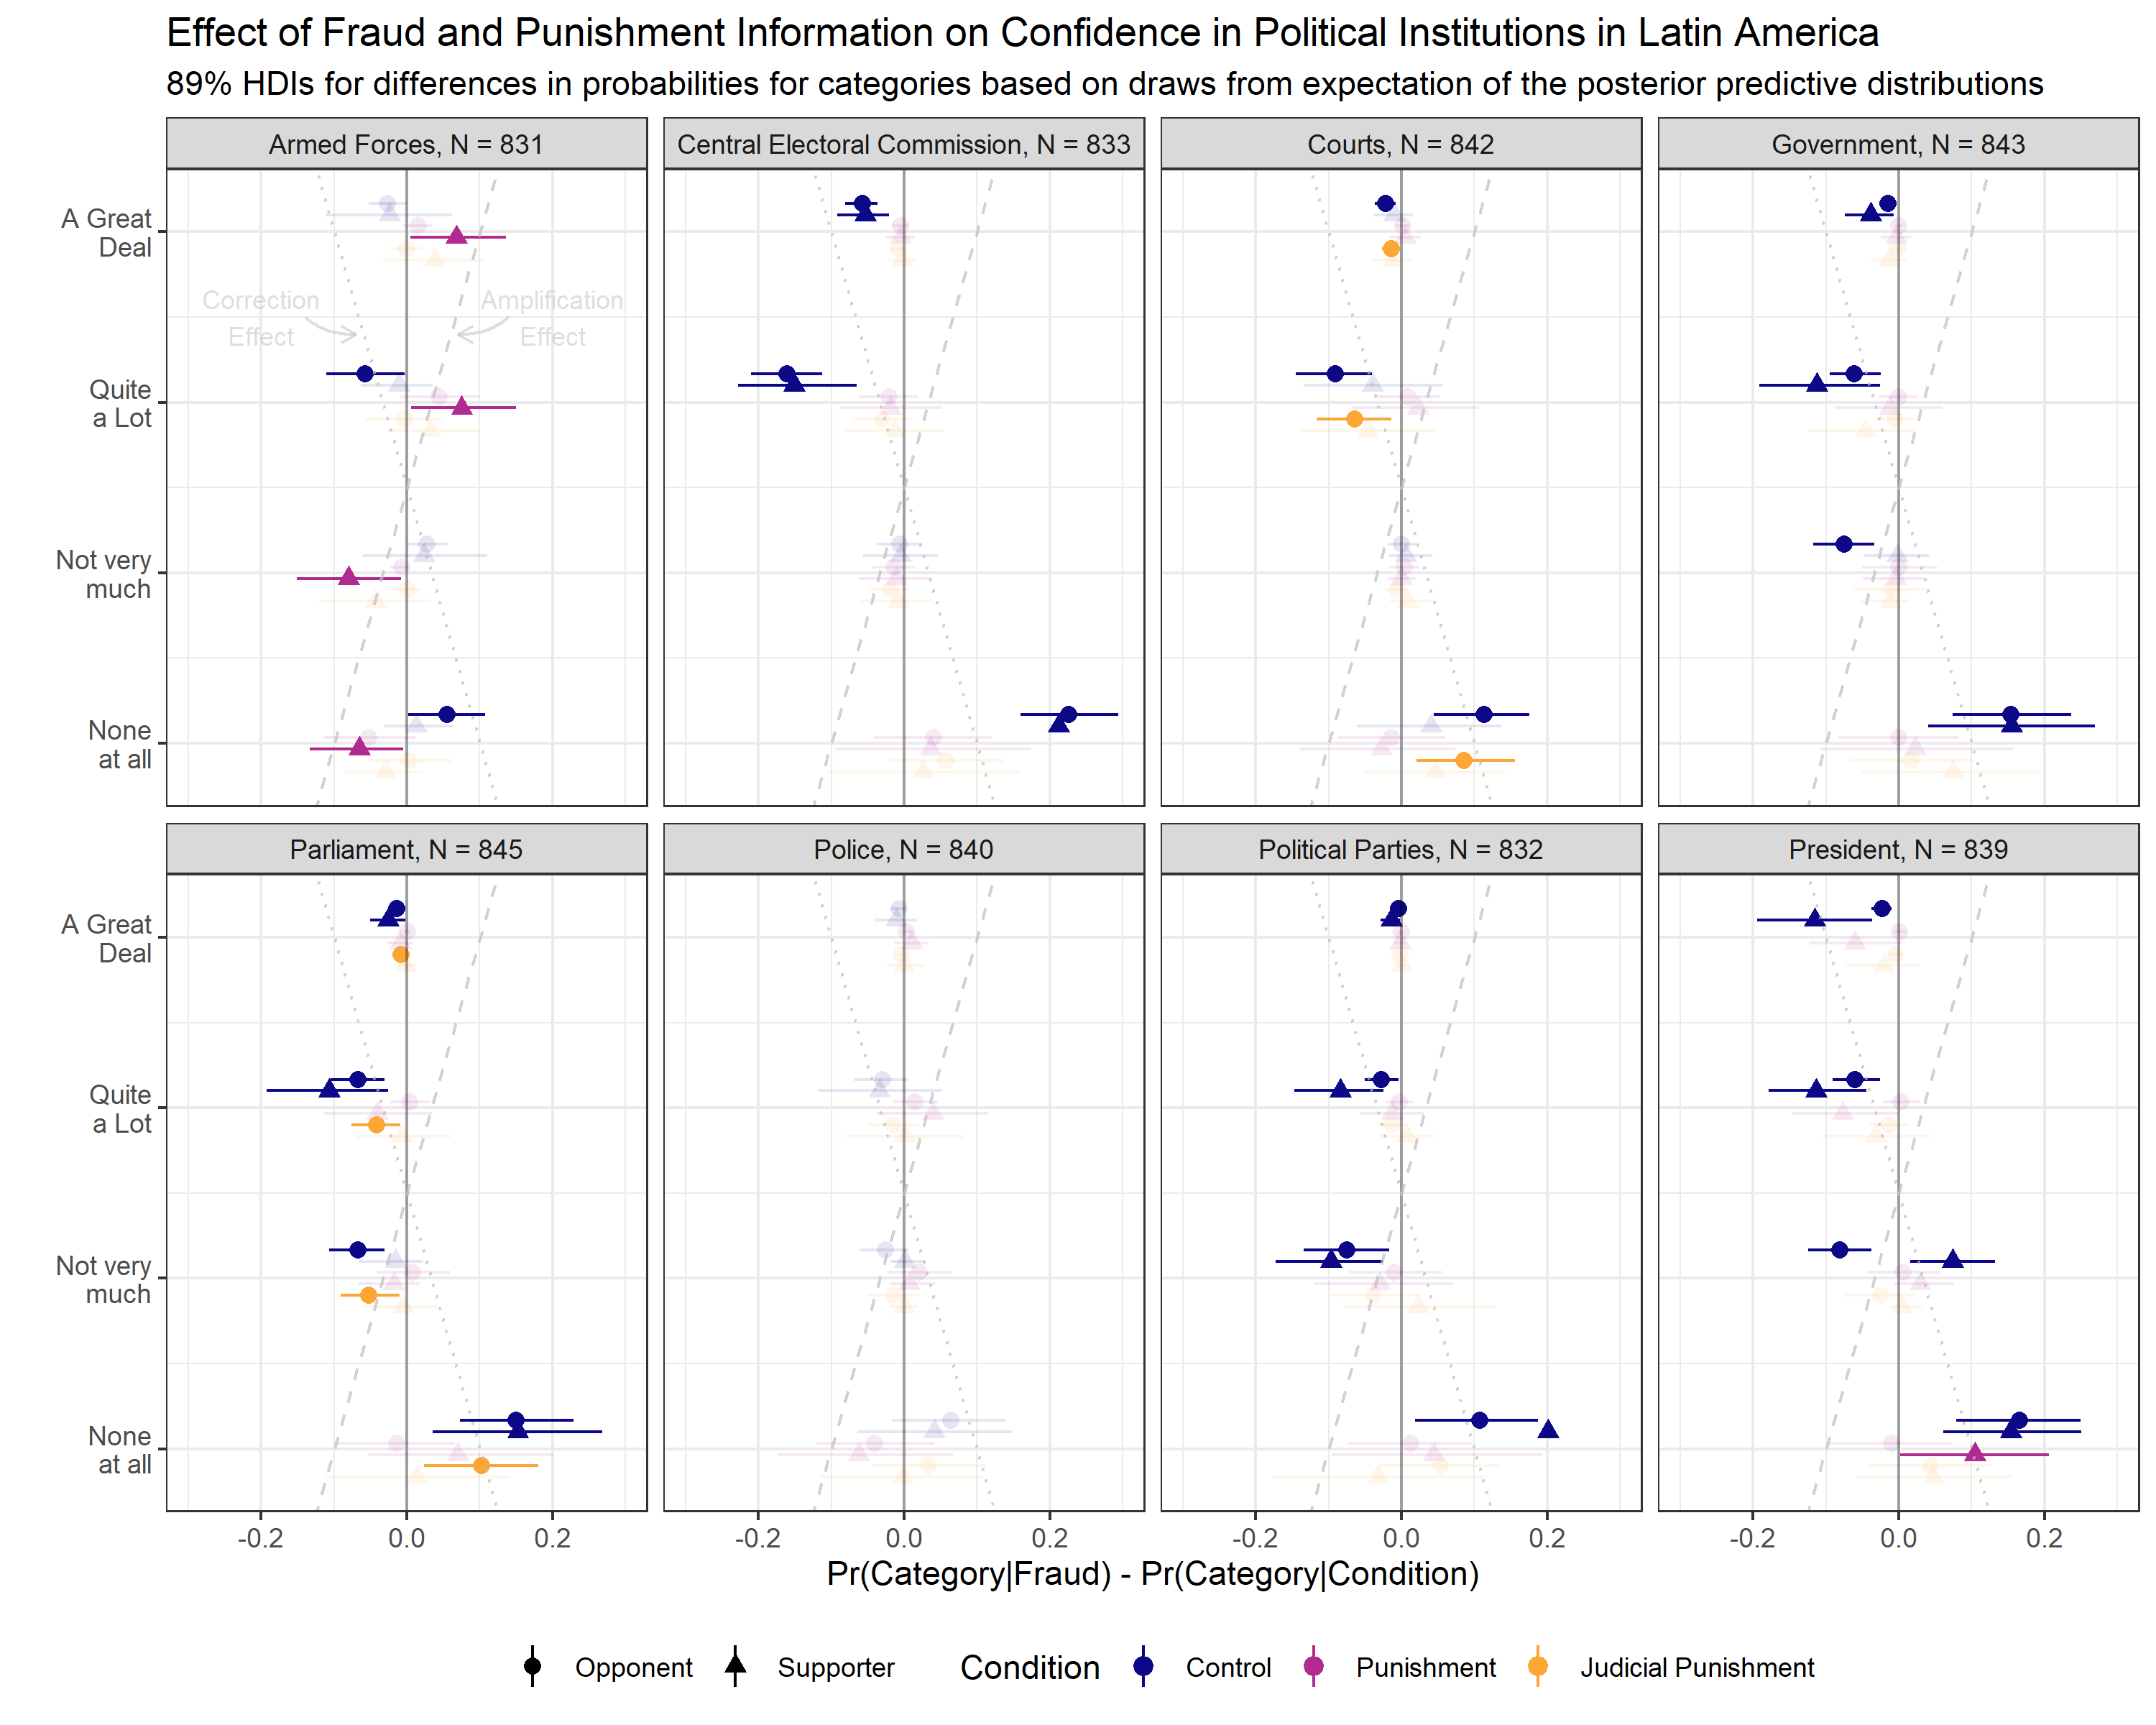
\includegraphics[width=\linewidth,trim=4 4 4 4,clip]{figs/la_hdi89_conditional.png}
%     \caption{Results for Latin America}
%     \singlespacing
%     \raggedright
%     \footnotesize{Notes: Positive values on the horizontal axis indicate that the probability of selecting a category is higher in fraud condition than in the other one. Conversely, negative values mean that respondent's probability to choose this was lower in fraud condition. Dashed (dotted) lines schematically depict the hypothesized relationships between categories, i.e. point estimates would loosely follow the pattern of the dashed (dotted) line if the relationship between trust and within-system response is amplifying (diminishing) the effect of fraud information on trust. Transparent point ranges include zero in the 89\% highest density interval.} 
%     \label{fig:het-la}
%     \end{figure}

To sum up, we find sufficient support for the first hypothesis, indicating the damaging effect of information about fraud on institutional trust across both samples. At the same time, the effect of within-system responses still remain more ambiguous. While adequate punishment of fraud perpetrators may decrease the negative effects of fraud information, and in certain conditions even amplify trust in political system, this effect is not universal and omnipresent across institutions. While we find both amplification and correction patterns in our analysis, we cannot clearly attribute it to either supporters or opponents as subgroups with potentially distinct information processing pathways.

As further robustness analysis, we restrict the sample based on the quality of responses as measured with the adequacy of the provided summary of the treatment, which is a post-treatment measure. While better-quality responses may help us in identifying the patterns clearer, introducing sample restrictions based on a post-treatment measure may have introduced further problems into the analysis.   
We also show that decline in trust in institutions is directly related and occurs through the decline in confidence in elections procedure with the help of mediation analysis. Lastly, we show that our results withstand alternative specifications for the supporter/opponent distinction, a crucial one in our theoretical discussion.  

%TO ADD HERE:
%
%- robustness crap %- discussion of sample size and hypothetical nature of the experiment to sweeten the small/insignificant effects fact - in Russia - fraud is not new, but the punishment would be less known. Hence -> stronger effects?- remove titles from plots?? - add notes/annotations to each figure 


%The respondents in Latin America were more likely to report less confidence in political institutions if they received information about electoral misconducts alone in comparison to receiving no such information. 



% We present the estimates from two model specifications: estimating effects for the entire sample, i.e. testing the first hypothesis, and the heterogeneous effects, estimating the effects of treatment conditional on the political affiliation of the respondent, i.e. testing the second hypothesis. We use all complete cases available for a particular institution, hence total sample sizes vary slightly across institutions. 

% Figure NN depicts, for each institution in question, the first differences in probabilities of selecting each category when evaluating the trust between receiving fraud information alone and another condition  - control or one of the punishment conditions. Hence, for each respected category depicted on the vertical axis the differences in probabilities would be positive when the respective predicted probability is larger in the fraud condition and negative when the probability of selecting the category is smaller in case only fraud information was presented to the respondents (or was supplemented with punishment information). 

%  For instance, respondents have, on average, 15 percentage points higher probability of reporting no support for government whatsoever when they are faced with information about fraud rather than with a neutral status quo scenario. At the same time, their probability of reporting some support to governemnt is smaller once they learn about fraud on the local level. Interestingly, fraud information led to no significant changes in reported trust in the armed forces in Latin America, which could be a result of clearer demarcation of this institution from the other actors in the political sphere. 

% The effects of retribution information is less straightforward: while the information about members of the commissions loosing their jobs seems to have no correcting effect on the trust in political institutions, the involvement of judiciary branch seems, to some extent, reinstate trust in parliament and courts themselves in Latin American countries. Still, 





\vspace{1cm}

\section*{Conclusion}

Acquiring credible information about electoral fraud can hold several attitudinal consequences for the relationship between citizens and their political system. The literature investigating the citizen-system nexus have focused on behavioral consequences of exposed cheating such as engaging in popular protests and violent uprisings (\citealt{Daxecker2012}). Regarding the electoral process itself, scholars have linked fraud information to negative evaluations of electoral quality (\citealt{Robertson2017}) and withdrawals of support from candidates that are allegedly involved in fraudulent practices (\citealt{Reuter2019}) and the regime that surged out of an allegedly fraudulent election (\citealt{Williamson2021}). The present article set out to theorize and explain the effects that acquiring credible information about electoral malpractice exerts on their confidence and diffuse support for the political system as a whole. 

In this article, we have provided first evidence that perceptions of election fraud lead to decays in levels of diffuse support for the political system as a whole among the citizenry. This spillover effect of election process-related perceptions to other components of the political system suggests that extrapolate process-related information even towards other institutions that are unrelated to electoral administration. Specifically, analyzing 48,953 respondents from Wave 7 (2017-2020) of the World Values Survey, respondents who perceive the election process of their country as less free and fair expressed lower levels of confidence in an array of political institutions even after rigorous covariate adjustment through statistical matching techniques. 

Second, we extended the focus of the simple citizen-system nexus and theorized about conditions that amplify or prevent such attitudinal spillover effects to occur. Specifically, we placed our theoretical scrutiny around the interventions of third-party stems actors and formulated two contrasting arguments on the moderating role of court convictions of alleged fraud perpetrators for the spillover effect of election fraud information. Last, we outlined the set up of a pre-registered online survey experiment to be conducted with respondents in Mexico and Russia which traces the causal mechanism behind the main spillover effect and its dependence on the occurrence of within-system interventions of courts as a consequence to exposed cheating. 

The theory and evidence presented in this article have a number of significant implications for developing democracies as well as contemporary authoritarianism. For instance, it has been shown that citizens who place higher levels of trust in their political system are more likely to turn out to vote (\citealt{WANG2016291}). Since active participation in institutionalized forms of democratic engagement is crucial for countries undergoing processes of democratic consolidation, our findings suggest that election fraud information can hinder the process of domestic democratization even in future electoral events that go beyond the impact on individual electoral contests. 

Second, our findings hold implications for the practice of election monitoring itself. Our article well aligns with a set of studies that have highlighted the cost among civil society when election observation missions expose cheating (\citealt{Daxecker2012}). Our preliminary findings suggest that when large-scale observation missions that are perceived and framed as credible players in the field claim election malpractice to be at place, such exposure may have detrimental effects that may hinder, rather than foster, the consolidation of a democratic society. This is especially relevant against the backdrop of widespread criticism that has been voiced against recent election observation missions proclaiming early conclusions about electoral malpractice that later do not uphold more intensive scrutiny (\citealt{Idrobo2020}). Our article suggests that the impact that such erroneous allegations about clean electoral process exerts on individuals should not be underestimated. 


\clearpage
\singlespace
\bibliographystyle{apsr} 
\bibliography{fraud_experiment}

\newpage
\appendix
\thispagestyle{empty}
\appendixpage
\startcontents[sections]
\printcontents[sections]{l}{1}{\setcounter{tocdepth}{2}}
\newpage
\renewcommand*{\thepage}{A\arabic{page}}
\renewcommand*{\thesection}{\Alph{section}.}
\renewcommand*{\thesubsection}{\alph{subsection}.}
% \renewcommand*{\thesubsubsection}{\alph{subsubsection}.}
\renewcommand\thefigure{A\arabic{figure}}   
\renewcommand\thetable{A\arabic{table}}  
\setcounter{figure}{0}
\setcounter{table}{0}
\setcounter{page}{1}





\section{Cross-National Evidence: Matching Analysis}

\subsection{Descriptive Statistics}
Table \ref{descr:matching} contains the summary statistics for complete cases in WVS data merged with the V-Dem Project data. 

\begin{table}[!htbp] \centering 
	\caption{Summary Statistics of Key Variables, World Values Survey Wave 7 (2017-2020).} 
	\label{descr:matching} 
	\begin{tabular}{@{\extracolsep{5pt}}lccccccc} 
		\\[-1.8ex]\hline 
		\hline \\[-1.8ex] 
		                               & \multicolumn{1}{c}{N} & \multicolumn{1}{c}{Mean} & \multicolumn{1}{c}{St. Dev.} & \multicolumn{1}{c}{Min} & \multicolumn{1}{c}{25\%} & \multicolumn{1}{c}{75\%} & \multicolumn{1}{c}{Max} \\ 
		\hline \\[-1.8ex] 
		% Confidence in Armed Forces & 48,953 & 2.876 & 0.951 & 1 & 2 & 4 & 4 \\ 
		% Confidence in the Police & 48,953 & 2.619 & 0.959 & 1 & 2 & 3 & 4 \\ 
		% Confidence in Courts & 48,953 & 2.558 & 0.962 & 1 & 2 & 3 & 4 \\ 
		% Confidence in Government & 48,953 & 2.385 & 0.996 & 1 & 2 & 3 & 4 \\ 
		% Confidence in Parliament & 48,953 & 2.182 & 0.948 & 1 & 1 & 3 & 4 \\ 
		% Confidence in Parties & 48,953 & 2.017 & 0.895 & 1 & 1 & 3 & 4 \\ 
		% Fraud Perception & 48,953 & 0.364 & 0.481 & 0 & 0 & 1 & 1 \\ 
		% Political Interest & 48,953 & 2.682 & 0.963 & 1 & 2 & 3 & 4 \\ 
		% Generalized Trust & 48,953 & 1.818 & 0.386 & 1 & 2 & 2 & 2 \\ 
		% Voting in National Elections & 48,953 & 1.557 & 0.822 & 1 & 1 & 2 & 4 \\ 
		% Sex & 48,953 & 1.512 & 0.500 & 1 & 1 & 2 & 2 \\ 
		% Age & 48,953 & 42.313 & 16.020 & 16 & 29 & 54 & 103 \\ 
		% Education & 48,953 & 4.043 & 1.479 & 1 & 3 & 5 & 6 \\ 
		% Employment Status & 48,953 & 3.192 & 2.044 & 1 & 1 & 5 & 8 \\ 
		% Household Income & 48,953 & 4.782 & 2.101 & 1 & 3 & 6 & 10 \\ 
		% Rural & 48,953 & 1.355 & 0.479 & 1 & 1 & 2 & 2 \\ 
		% Political Discussion & 48,953 & 2.220 & 0.647 & 1 & 2 & 3 & 3 \\ 
		Confidence in Armed Forces     & 42,586                & 2.865                    & 0.945                        & 1                       & 2                        & 4                        & 4                       \\ 
		Confidence in the Police       & 42,586                & 2.629                    & 0.943                        & 1                       & 2                        & 3                        & 4                       \\ 
		Confidence in Courts           & 42,586                & 2.568                    & 0.941                        & 1                       & 2                        & 3                        & 4                       \\ 
		Confidence in Parliament       & 42,586                & 2.187                    & 0.926                        & 1                       & 1                        & 3                        & 4                       \\ 
		Confidence in Government       & 42,586                & 2.384                    & 0.984                        & 1                       & 2                        & 3                        & 4                       \\ 
		Confidence in Parties          & 42,586                & 2.034                    & 0.874                        & 1                       & 1                        & 3                        & 4                       \\ 
		Confidence in Companies        & 42,586                & 2.398                    & 0.851                        & 1                       & 2                        & 3                        & 4                       \\ 
		Confidence in UN               & 42,586                & 2.445                    & 0.943                        & 1                       & 2                        & 3                        & 4                       \\ 
		Confidence in Banks            & 42,586                & 2.563                    & 0.930                        & 1                       & 2                        & 3                        & 4                       \\ 
		Confidence in WTO              & 42,586                & 2.439                    & 0.911                        & 1                       & 2                        & 3                        & 4                       \\ 
		Confidence in World Bank       & 42,586                & 2.419                    & 0.948                        & 1                       & 2                        & 3                        & 4                       \\ 
		Fraud Perception               & 42,246                & 2.841                    & 1.028                        & 1                       & 2                        & 4                        & 4                       \\ 
		Fraud Perception (binary)      & 42,586                & 0.651                    & 0.477                        & 0                       & 0                        & 1                        & 1                       \\ 
		% Fraud Perception (Alternative) & 42,586 & 0.865 & 0.342 & 0 & 1 & 1 & 1 \\ 
		% fraud1d2 & 42,586 & 0.326 & 0.469 & 0 & 0 & 1 & 1 \\ 
		Political Interest             & 42,586                & 2.390                    & 0.955                        & 1                       & 2                        & 3                        & 4                       \\ 
		Generalized Trust              & 42,246                & 0.202                    & 0.401                        & 0                       & 0                        & 0                        & 1                       \\ 
		Female                         & 42,246                & 0.495                    & 0.500                        & 0                       & 0                        & 1                        & 1                       \\ 
		Age                            & 42,586                & 41.634                   & 15.832                       & 16                      & 28                       & 54                       & 103                     \\ 
		Family Savings                 & 42,586                & 2.049                    & 0.902                        & 1                       & 1                        & 2                        & 4                       \\ 
		Rural                          & 42,246                & 0.339                    & 0.473                        & 0                       & 0                        & 1                        & 1                       \\ 
		Perceived Political Corruption & 42,586                & 7.736                    & 2.423                        & 1                       & 6                        & 10                       & 10                      \\ 
		V-Dem Election Integrity       & 42,586                & 0.618                    & 0.255                        & 0.053                   & 0.435                    & 0.856                    & 0.969                   \\ 
		\hline \\[-1.8ex] 
	\end{tabular} 
\end{table} 

\begin{itemize}
	\item Confidence in political institutions is measured on a 1 to 4 scale, with 1 meaning \textit{None at all} and 4 depicting \textit{A great deal}.
	\item Political interest is measured on a 1 to 4 scale, with 1 meaning \textit{Not at all interested} and 4 depicting \textit{Very interested}.
	\item Generalized trust is a binary indicator, with 0 meaning \textit{Need to be very careful} and 1 depicting \textit{Most people can be trusted}.
	\item Fraud perception is measured in WVS on a 1 to 4 scale based on the agreement with the following statement: "How often in country's elections: Votes are counted fairly", with 1 meaning \textit{Not at all often} and 4 depicting \textit{Very often}. 
	\item Fraud perception (binary) is the variable used in our matching analysis and is a binary indicator, with 0 being comprised of \textit{Not at all often} and \textit{Not often} and 1 of \textit{Fairly often} and \textit{Very often} answers to the respective WVS question. 
	\item Family savings during past year is measured on a 1 to 4 scale, with 1 indicating \tetxit{Save money}, 2\textemdash\textit{Just get by}, 3\textemdash\textit{Spent some savings and borrowed money}, and 4\textemdash\textit{Spent savings and borrowed money}.  
	\item Perceived Political Corruption is measured on a 1 to 10 scale, with 1 meaning \textit{There is no corruption in my country} and 10 depicting \textit{There is abundant corruption in my country}.
	\item V-Dem Election Integrity is the clean elections index scaled to range from 0 (lowest score) to 1 (highest score).
	      
\end{itemize}

\subsection*{Matching Analysis}
We now trace further empirical implications of our theory on a broader sample. Specifically, we test whether the proposed mechanism is in line with evidence from survey data from a heterogeneous country setting using statistical matching techniques for causal inference. To evaluate our central hypothesis of attitudinal spillover, we investigate whether effects of election fraud perceptions on diffuse support for political institutions that are unrelated to electoral administration also hold in a larger sample and a more heterogeneous country setting. To this end, we leverage data from the World Values Survey, a large-scale cross-national survey program relying on nationally representative samples providing time-series data between 1981-2020. 

While survey items relating to Easton's (1965, 1975) concept of diffuse support are part of the core questionnaire and asked consistently throughout all waves, a comprehensive battery of questions assessing respondent's perceptions of their country's electoral integrity has not been introduced before Wave 6 (2010-2014, c.f. \citealt{Norris2014}). Because perceptions of electoral fraud are not randomly assigned among respondents, individuals may differ from each other in ways that are related to their fraud perception as well as their diffuse support for political institutions. The World Values Survey includes a rich set of covariates that make it possible to condition on possible differences between individuals. 

After screening the data files, we noted that in particular Wave 7 (2017-2020) of the cumulative data file provides questions on issues that are particularly relevant for potential confounding mechanism that we are confronted with in the study of fraud perceptions and diffuse support. In particular, one can imagine that attitudes towards broader issues such as political corruption \textit{in general} may locate individuals on scales measuring perceptions of practices of election day fraud and confidence in political institutions. Moreover, citizens' levels of \textit{generalized trust} in the world may condition perceptions of election day events and the particularities of a political system (c.f. Keele 2007). The covariates that we employ are `pre-treatment' in the sense that they either portray socio-demographic characteristics that are unaffected by respondents' evaluations of election day practices or report more generalized attitudes that are likely to be preceding in the causal chain when explaining `treatment' variation of fraud perceptions.\footnote{One issue with our procedure is that the attitudinal measures are not strictly preceding the main variables of interest and might thus be \textit{affected} by fraud perceptions and confidence in institutions rather than \textit{predicting} `treatment' status. We report estimates including the attitudinal measures, but note that the results are robust to model specifications which only use socio-demographic information for covariate adjustment.} We hence exploit data from Wave 7 of the World Value Survey covering 48 different countries across democratic and electoral authoritarian regimes. Table A1 in the appendix provides an overview over our used variables and countries included in the analysis. Our final models include a total number of 48,953 respondents. 

Regarding our measures of fraud perceptions and diffuse political support, we choose those variables that provide the closest approximation of the measurements imposed in our survey experiment to ensure a direct test of external validity. The World Values Survey measures diffuse support through asking respondents: \textit{“I am going to name a number of organizations. For each one, could you tell me how much confidence you have in them: is it a great deal of confidence, quite a lot of confidence, not very much confidence or none at all?”}. We include responses to the same seven institutions that we collect data on in our survey experiment. On the explanatory side, rather than assigning participants to different kinds of fraud information, respondents here are asked about a battery of items covering various aspects of electoral integrity throughout the whole electoral cycle. We focus on the question that is most closely related to the mechanism of election day ballot fraud of our survey experiment stating: \textit{“In your view, how often do the following things occur in this country's election: Votes are counted fairly.”}. Answers are collected on a four-point scale covering “very often”, “fairly often”, “not often” and “not at all often”. To straightforwardly discriminate `treatment' and `control' groups, we collapse this variable into a binary indicator with each group covering two response categories.  

\begin{figure}[H]
	\caption{Covariate Balance Before and After Sample Adjustment Using Coarsened Exact Matching.}
	\centering
	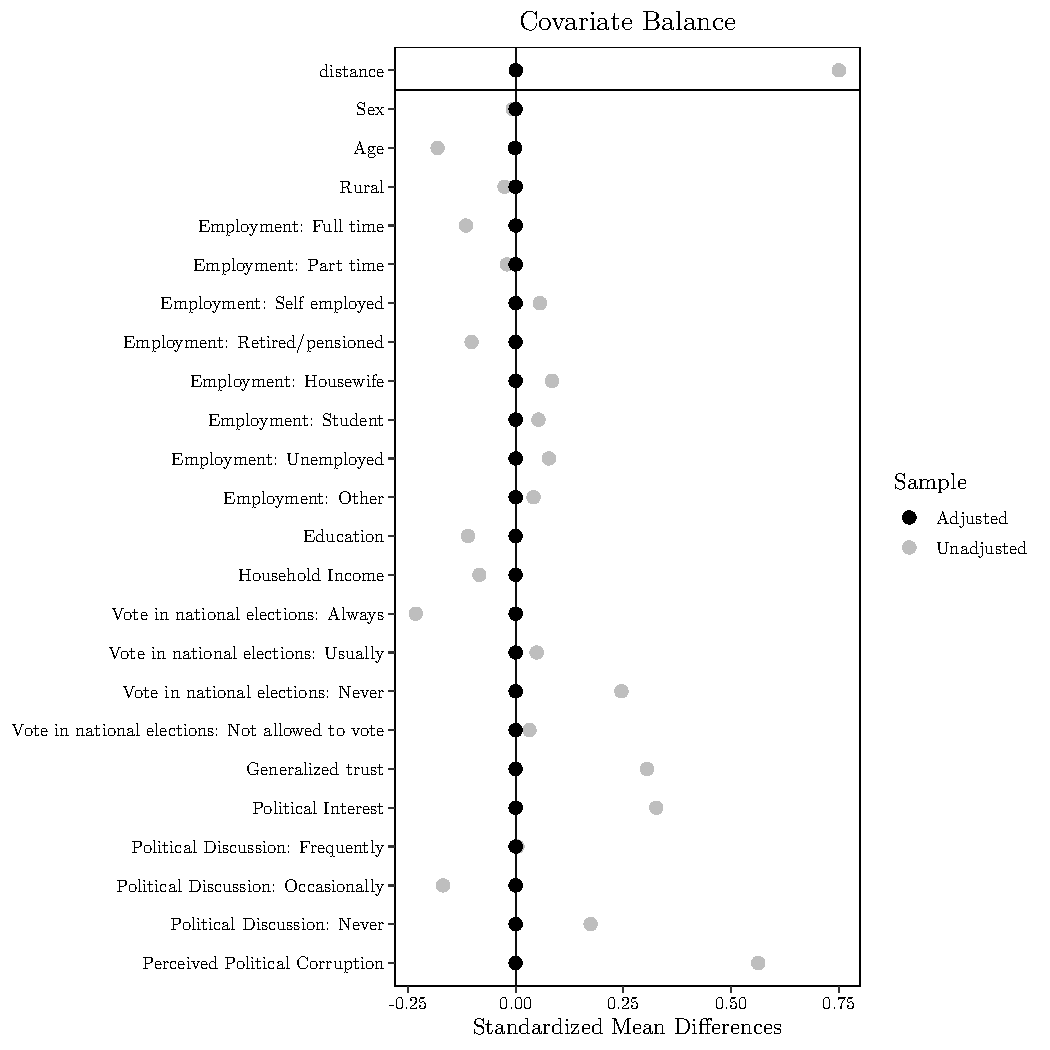
\includegraphics[width=0.9\linewidth]{covbalance_cem.pdf}
	\label{fig:balance}
\end{figure}

We apply matching as our main method for covariate adjustment in order to avoid parametric assumptions that stem from more conventional statistical models for cross-sectional data and present causal estimates on the relation between election fraud perceptions and diffuse political support. Statistical matching is commonly described as “the most developed [..] strategy for causal analysis in observational studies” (\citealt{Pearl2010}) and the literature on causal inference from cross-sectional data has produced a large range of algorithms and approaches to achieve balanced datasets that are free of usually embedded  parametric assumptions. 

We employ two different strategies for our inferences. First, we exploit propensity scores as the most popular similarity criterion and pre-select a subset of our data in which `treated' and `control' units most closely resemble each other in pre-treatment characteristics. The gold standard in constructing balanced data is exact matching, though usually disregarded because it produces a large share of cases that are left unmatched creating trouble for effect identification stemming from small sample sizes. In our particular case in which we exploit a dataset with over 48,000 data points, we can nevertheless rely on exact matches and construct a balanced dataset covering 580 individuals. Second, the use of propensity scores as a characteristic to match on has been criticized more generally (\citealt{King2019}). As a second approach to causal inference, we rely on coarsened exact matching (CEM) as developed by \citet{Iacus2012} which has been proposed as an alternative to propensity score-based methods and has the potential to reduce large parts of model dependence, bias and variance that are left unaccounted by conventional matching algorithms. We compared these two approaches to a number of other algorithms for sample adjustment using matching and find these provide us with the best covariate balance by far. 

Figure 1 presents measures of covariate balance between those individuals falling into the `fraud' and `no fraud' perception condition before and after our sample adjustment. For each covariate that we match on, we report the standardized bias as measured by the difference in means between both groups of individuals scaled by the pooled standard deviation. Dots to the right (left) of the dashed vertical line are indicative of a higher incidence of respective characteristics among those individuals that perceive the elections of their country as unfair (fair). As indicated by the grey circles, fraud perceptions are most prevalent among those individuals that report to never turn out to vote, obtain low levels of interpersonal trust, and perceive political corruption at large scale in their country. 

\begin{table}[]
	\caption{Matching Estimates: Effect of Fraud Perceptions on Confidence in Political Institutions.}
	\singlespace
	\begin{tabular}{llllccccc}
		\hline
		& \multicolumn{2}{c}{Na{\"i}ve Estimate}                                         & \multicolumn{1}{c}{}          & \multicolumn{2}{c}{Coarsened Exact Matching} &                      & \multicolumn{2}{c}{Exact Matching}          \\
		                              & \multicolumn{1}{c}{\textit{Coef.}} & \multicolumn{1}{c}{\textit{Std.Err.}} & \multicolumn{1}{c}{\textit{}} & \textit{Coef.}       & \textit{Std.Err.}    & \textit{}            & \textit{Coef.}       & \textit{Std.Err.}    \\ \cline{2-3} \cline{5-6} \cline{8-9} 
		\textit{Real Spillover}       &                                    &                                       &                               & \multicolumn{1}{l}{} & \multicolumn{1}{l}{} & \multicolumn{1}{l}{} & \multicolumn{1}{l}{} & \multicolumn{1}{l}{} \\
		Effect on: Armed Forces       & -0.432                             & 0.019                                 &                               & -0.508               & 0.073                &                      & -0.384               & 0.151                \\
		Effect on: Police             & -0.526                             & 0.019                                 &                               & -0.671               & 0.074                &                      & -0.681               & 0.153                \\
		Effect on: Press              & -0.428                             & 0.019                                 &                               & -0.366               & 0.074                &                      & -0.215               & 0.155                \\
		Effect on: Courts             & -0.601                             & 0.019                                 &                               & -0.803               & 0.075                &                      & -0.718               & 0.153                \\
		                              &                                    &                                       &                               &                      &                      &                      &                      &                      \\
		\textit{Endogenous Spillover} &                                    &                                       &                               &                      &                      &                      &                      &                      \\
		Effect on: Government         & -0.694                             & 0.020                                 &                               & -0.709               & 0.074                &                      & -0.739               & 0.153                \\
		Effect on: Parliament         & -0.660                             & 0.020                                 &                               & -0.745               & 0.076                &                      & -0.514               & 0.155                \\
		Effect on: Political Parties  & -0.560                             & 0.020                                 &                               & -0.535               & 0.076                &                      & -0.434               & 0.158                \\ \hline
		Covariate Adjustment          & \multicolumn{2}{c}{$\surd$}                                                & \multicolumn{1}{c}{}          & \multicolumn{2}{c}{$\surd$}                  &                      & \multicolumn{2}{c}{$\surd$}                 \\
		$N$                             & \multicolumn{2}{c}{48,953}                                                 & \multicolumn{1}{c}{}          & \multicolumn{2}{c}{2,475}                    &                      & \multicolumn{2}{c}{580}                     \\ \hline
	\end{tabular}
	\textit{Note: Na{\"i}ve estimates are drawn from ordinal logistic mixed models nesting 52,105 individuals in 48 countries fitted with maximum likelihood estimation. Matching results are drawn from exact and coarsened exact matching with postmatching regression adjustment through parametric ordinal logistic models. Coefficients represent average treatment effects (ATE).}
\end{table}

Notably, these differences are almost completely reduced after pruning the data as a result of our matching algorithms, as indicated by the black dots. Standardized bias is close to zero for all covariates in the adjusted sample, and matched groups are highly similar on any of their observed characteristics.\footnote{This picture equivalently holds for standardized bias reduction using propensity-score based exact matching.} Hence, in our analysis, the remaining differences on diffuse political support that are still observed between both groups on our fraud indicator can be plausibly attributed to differences in election day fraud perceptions. 

Table 2 presents the effect estimates. The first column presents na{\"i}ve estimates drawn from an ordinal logistic mixed model on the whole dataset using available covariates as control variables. Columns 2 and 3 present the results of our matching estimators. All coefficients provide estimates of the average treatment effect (ATE). Across specifications, we find robust support for our main hypothesis of attitudinal spillover. Perceived prevalence of election day ballot fraud in the federal elections of one's country shows to robustly decrease confidence in political institutions that are unrelated to electoral administration. These effects hold for those institutions that are potentially thought to be related to electoral malpractice (endogenous spillover) as well as for those institutions that are exogenous to election day procedures (genuine spillover effect). 


\clearpage
\section{Survey Experiment} 
\subsection{Descriptive Statistics}
\onehalfspacing


Tables \ref{descr:russia} and \ref{descr:la} contain summary statistics for the survey responses in Russia and Latin America for the observations we used in the main analysis, for each treatment group. As per the pre-registration analysis plan, we exclude any unfinished interviews and cases where the interviews were finished in under 3 minutes to control for data quality. To represent the target population, i.e. potential voters, we also remove responses from respondents under 18 and non-citizens of target countries, which was also set as a restriction for participation at the recruitment stage. \footnote{While in PAP we also discuss the manual quality control using attention checks and removing cases that depict no meaningful engagement with treatment, for the main analysis, we refrain from excluding observations based on this post-treatment criteria. We replicate the analysis and explore data quality variation in the following section, and the results hold and the effects are more pronounced for the samples with higher-quality responses
	% atment; cases with answers that contained no meaningful text were excluded. Additionally, the cases with summaries of a scenario different to the one given to the respondent are treated as lack of meaningful engagement. For further details, please consult Data quality subsection.
} We may conclude that randomization across conditions contributed to covariate balance, as we observe no significant differences across the treatment groups. As expected, our sample consists of primarily young, urban, middle-to-high educated people in both Russia and Latin America.   

\subfile{tables/descr_ru}
\subfile{tables/descr_la}


\clearpage
\subsection{Data Quality}

\onehalfspacing

Since our target population of study would be voting-eligible population in the countries of Mexico, Columbia, and Russia, our sampling strategy implies using these as pre-requisites for participation in the survey. Hence, we excluded all the cases where the reported age of the respondent was below 18 years old, which still occurred despite the crowd-sourcing platform restriction of 18 years old, and the cases where the respondent claimed to not be the citizen of the respective country, also occurring despite the restrictions set on the crowd-sourcing platform. 

We are limiting the analysis to complete cases only, which requires us to have a closer look at the dropout and sample response when discussing data quality. As we have relied on the crowd-sourcing platforms for participant recruitment, participants were paid for completing the survey. Given that participants only received the payment upon completion of the survey, we obtained a 95\% completion rate in Russia and 92\% in Latin American countries.

Apart from the absolute number of completed surveys, a valid concern regarding dropout rate could be that it varies over our experimental conditions, introducing bias into the sampling procedure and completed cases. As evidenced by the tables below, there seem to be no systematic differences in the dropout rates across the experimental conditions, i.e. dropout rates right after reading the treatment condition. 

\subfile{tables/dropout_ru}
\subfile{tables/dropout_la}

\clearpage

Furthermore, as per the pre-analysis plan, we have excluded cases where the survey was completed in under 3 minutes, as reading and answering all the questions meaningfully in a shorter amount of time seems to be unrealistic.
For reference, we provide summary statistics for the time required for completing the treatment text page for the finished interviews, which required summarizing the text, and statistics for institutional trust evaluation page. While small variations in completing the treatment page may be related to small differences in the length of treatment conditions, we can conclude that the lower bound of 3 minutes seems reasonable for each condition for any of them. 

% With this being post-treatment criteria, which may arise  we replicate the analysis without excluding any observations based on these criteria. 


\subfile{tables/time_required_ru}
\subfile{tables/time_required_la}

\clearpage

We have also manually coded the summaries to differentiate the responses by the levels of engagement to allow for robustness checks. We have distinguished between \textit{complete summaries}, which contained the condition-specific part of the treatment, \textit{incomplete summaries}, where the responses described only a part of the treatment message but lack the crucial info for that condition;  \textit{responses} to the texts which allowed us to expect that the treatment text was read; \textit{copy-paste} of one or multiple paragraphs from the treatment text in the questionnaire, and \textit{unacceptable answer}, which does not allow us to observe any meaningful engagement with the treatment (e.g., a sequence of random characters). While we avoid removing any data based on this criterion in the main analysis due to potential introduction of post-treatment bias though case selection, we report the analysis on the restricted samples in robustness section, and the results show that our findings hold also when relying on a more restrictive approach to data preparation. Furthermore, for the cases where we received complete summaries, i.e. we can be certain that the treatment was read, the effects are particularly pronounced. 

\subfile{tables/manual_quality_ru}
\subfile{tables/manual_quality_la}

\newpage
\subsection{Results}


In the main text, we only present the plots with the most relevant quantities of interest for our purposes (see figures \ref{fig:main} and \ref{fig:het}). This section contains further details on the results, such as tables with models' estimates for the reference purposes and additional figures with quantities of interest calculated with these models such as raw probabilities for each treatment group. 

\subsubsection*{Political Institutions}

\subfile{tables/ol_main_la_pol_872}

\clearpage

\subfile{tables/ol_main_ru_pol_1223}


\subfile{tables/ol_cond_la_pol_872}

\newpage

\subfile{tables/ol_cond_ru_pol_1223}


\clearpage

Figures below present the intermediate quantity of interest--the probabilities of choosing one of four categories for trust--for each of the four conditions. These were obtained from the  draws from the expectation of the posterior predictive distributions, and we show the 89\% highest-density continuous interval for probabilities of choosing respective categories. These are the quantities we used to produce the main plots in the paper based on models in tables \ref{tab:ol}, yet exploring the raw probabilities may also be of interest.  (without any exclusions), while same plots for restricted samples are available in replication material (as the general trends persist). 

Besides the trends discussed in the main text, we can observe that, oftentimes, trust in political institutions in our samples is low regardless of the treatment conditions: the probabilities corresponding to the highest trust category is, generally, the lowest for all institutions across all treatment conditions. The exceptions are trust in the President and Armed Forces in Russia, which is in line with the narrative observed in the media of that time. 

\begin{figure}[H]
	\centering
	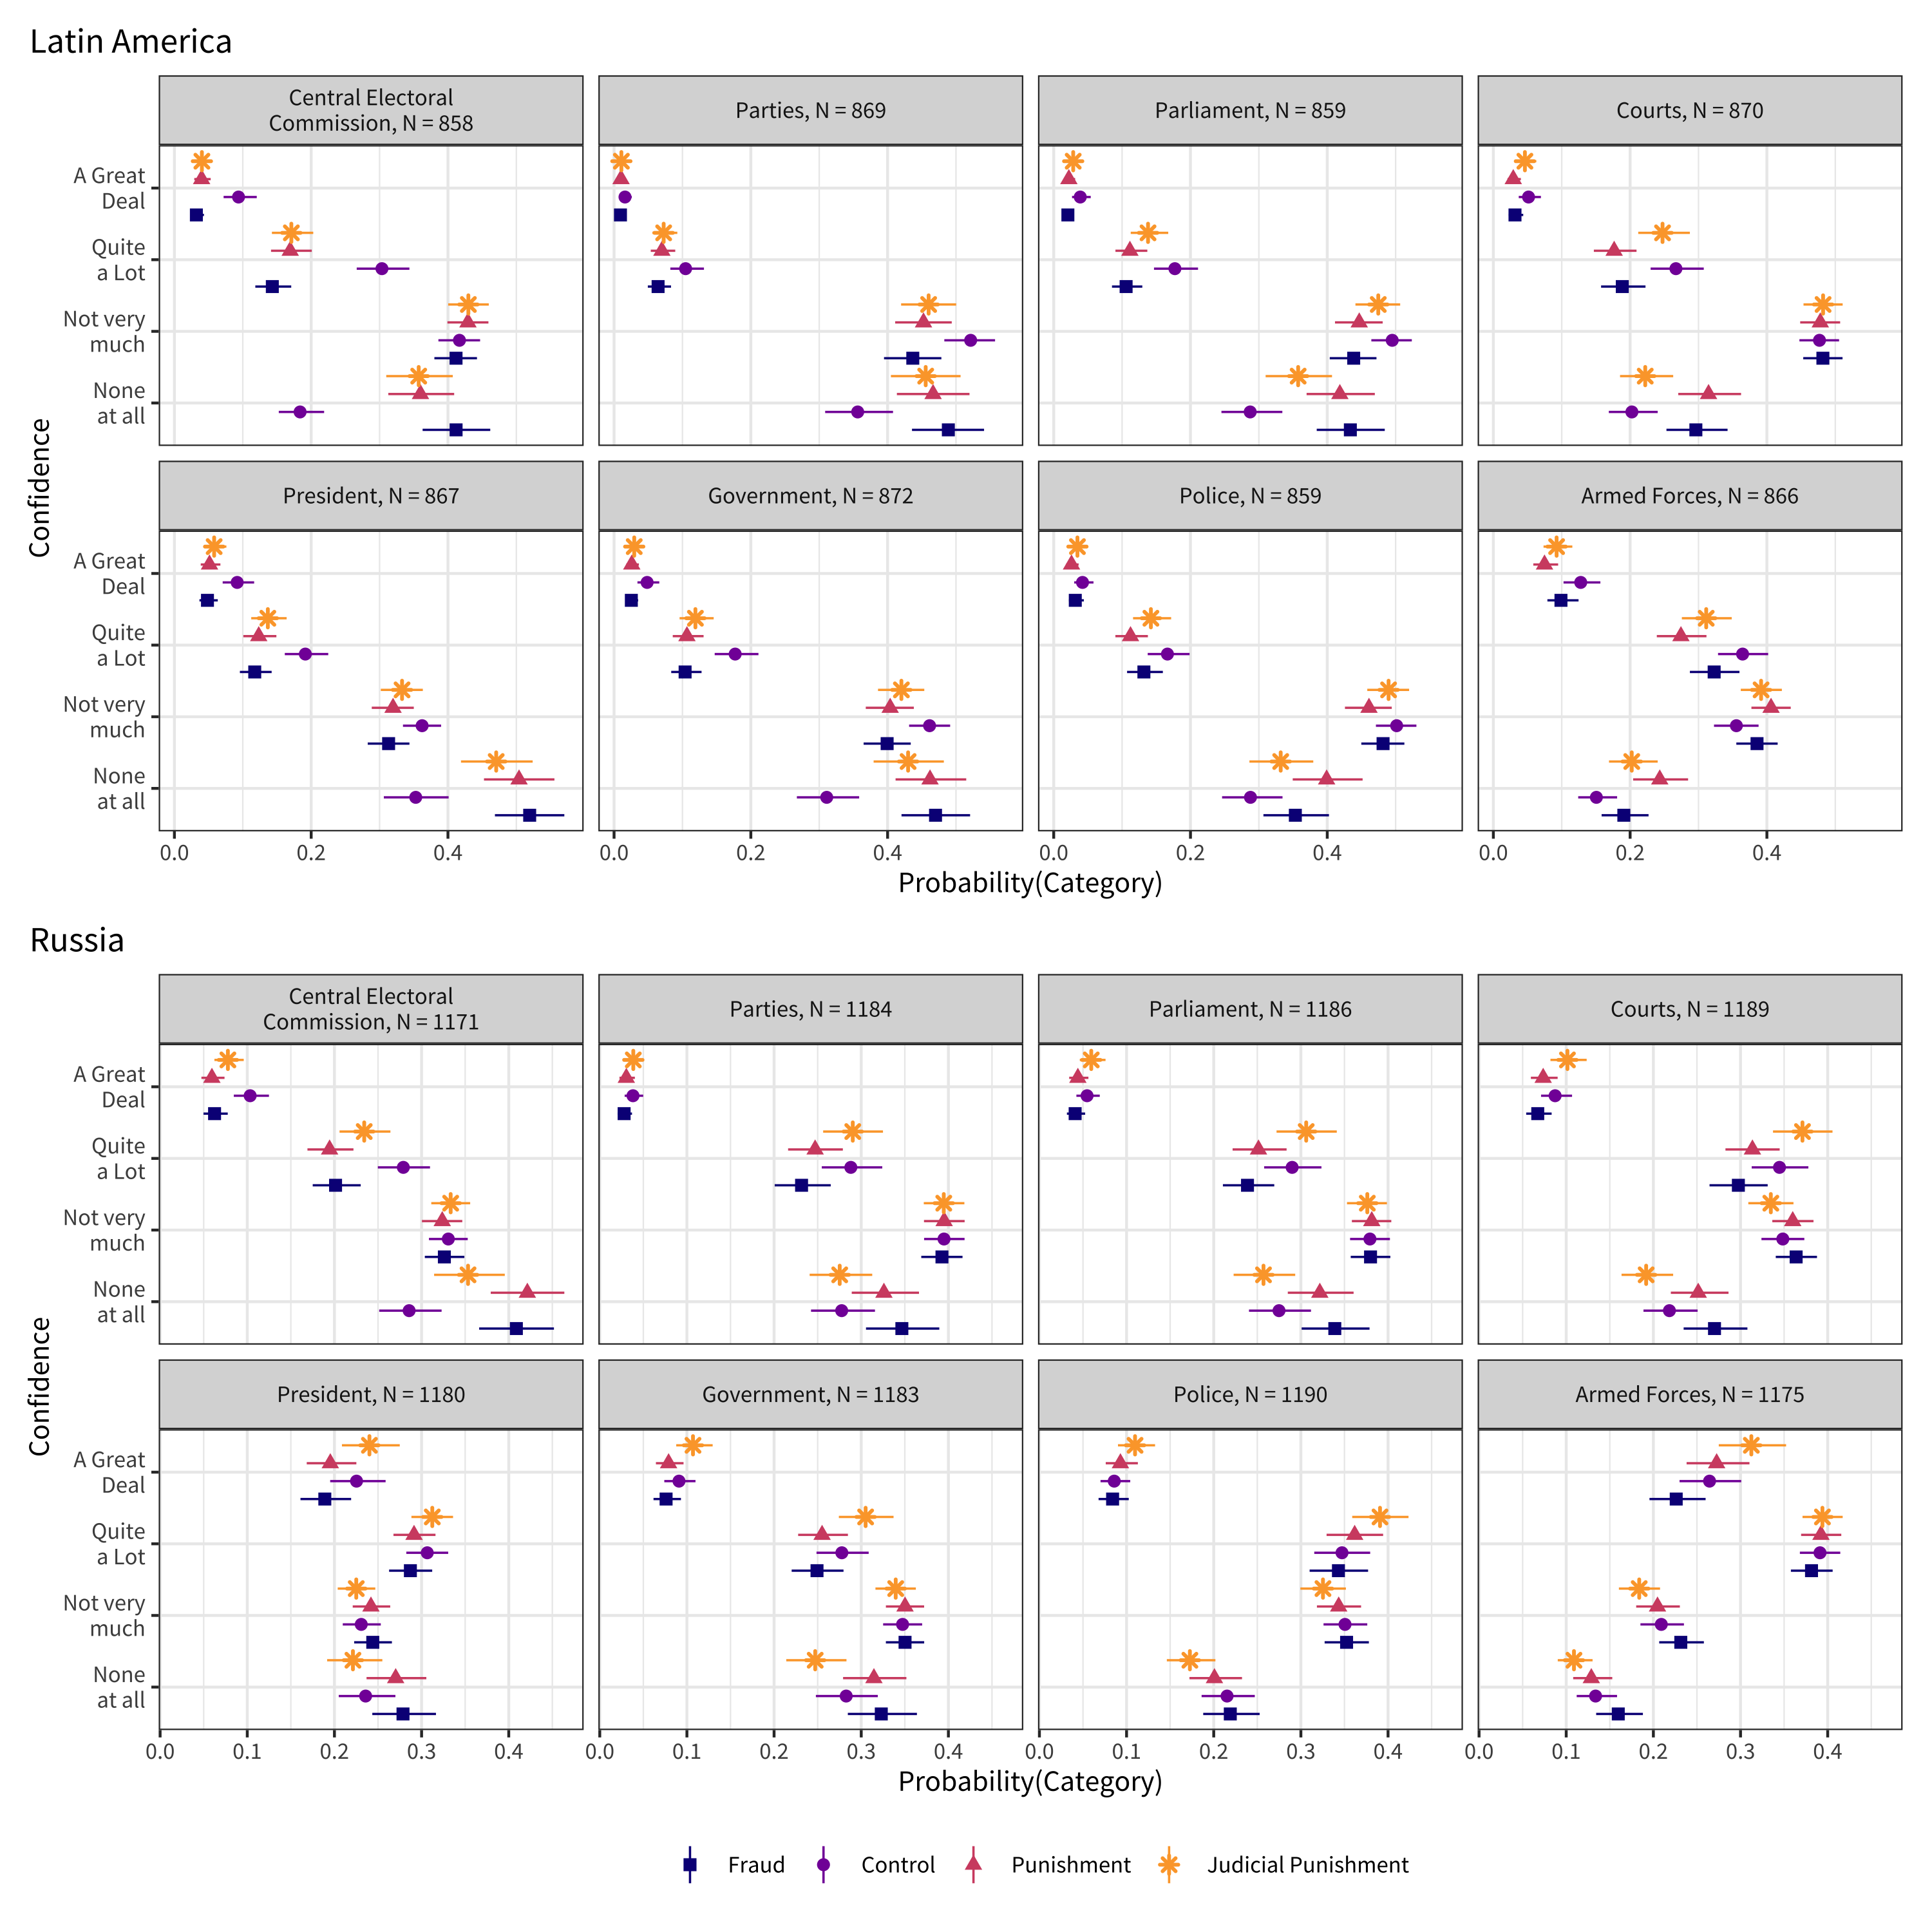
\includegraphics[width=\linewidth,trim=4 4 4 4,clip]{figs/probs_hdi89_1.png}
	\caption{The Effect of Exposure to Fraud and Punishment Information on Confidence in Political Institutions.  \\
		\footnotesize{Notes: Plots depict medians and 89\% highest-density continuous interval for probabilities of choosing respective categories based on draws from the expectation of the posterior predictive distributions. Probabilities are calculated based on ordered logit model estimates described in main analysis.
			Transparent point ranges include zero in the 89\% HDCI.
	} }
	\singlespacing
	\raggedright
\end{figure}
    
    

\clearpage

\subsubsection*{Non-Political Institutions}

We ask the respondents to evaluate their trust in non-political institutions as well as in political upon reading the treatment text, which allows us to evaluate the limitations of the theory clearer. As we can observe from the estimates in the table below, the treatment groups do not differ significantly in their confidence in non-political institutions in both Latin America and Russia. The only exception seems to the Russian sample and the effect of court intervention as response to fraud in comparison to fraud alone (i.e., the baseline condition). Judicial punishment information seems to increase trust in companies, banks, environmental organisations, and the World Trade Organisation, but not in the United Nations or the World Bank. One could argue that this could be an evidence of a spillover effect, which goes beyond the political sphere and exists for entities that are not portrayed negatively and "pro-Western" in the Russian media. The fact that we observe it specifically in Russia and only in response to the message about the intervention of another political institution could also be interpreted as evidence for the belief updating mechanism in evaluations. As this information may go against the general expectations of the systems' responses to election manipulation in an autocratic state, judicial interventions' consistent restorative effect on trust for various institutions indicates that respondents seem to have updated their beliefs rather than disregard the information that goes counter their current perceptions. 

\subfile{tables/ol_main_la_npol_872}
\subfile{tables/ol_main_ru_npol_1223}


\normalsize

\clearpage
\section*{Robustness Checks}

This section contains the results of various robustness checks and investigation of further observable implications.

\subsection*{Data Quality Restrictions}

% \footnotesize
% \subfile{tables/ol_main_la_pol_854}

% \clearpage
% \subfile{tables/ol_main_ru_pol_1203}

First, we only focus on the cases where the respondents in our survey have indicated at least minimal degree of meaningful involvement with the treatment text. We thus remove the few cases where we could not conclude that the respondent has read the text based on the attention check text, e.g. if the summary consisted of a sequence of random symbols. We replicate the main analyses, and figures \ref{fig:main-2} and \ref{fig:main-6} contains the results. As we can see, in both countries the results from the main analysis hold. 

\begin{figure}[H]
	\centering
	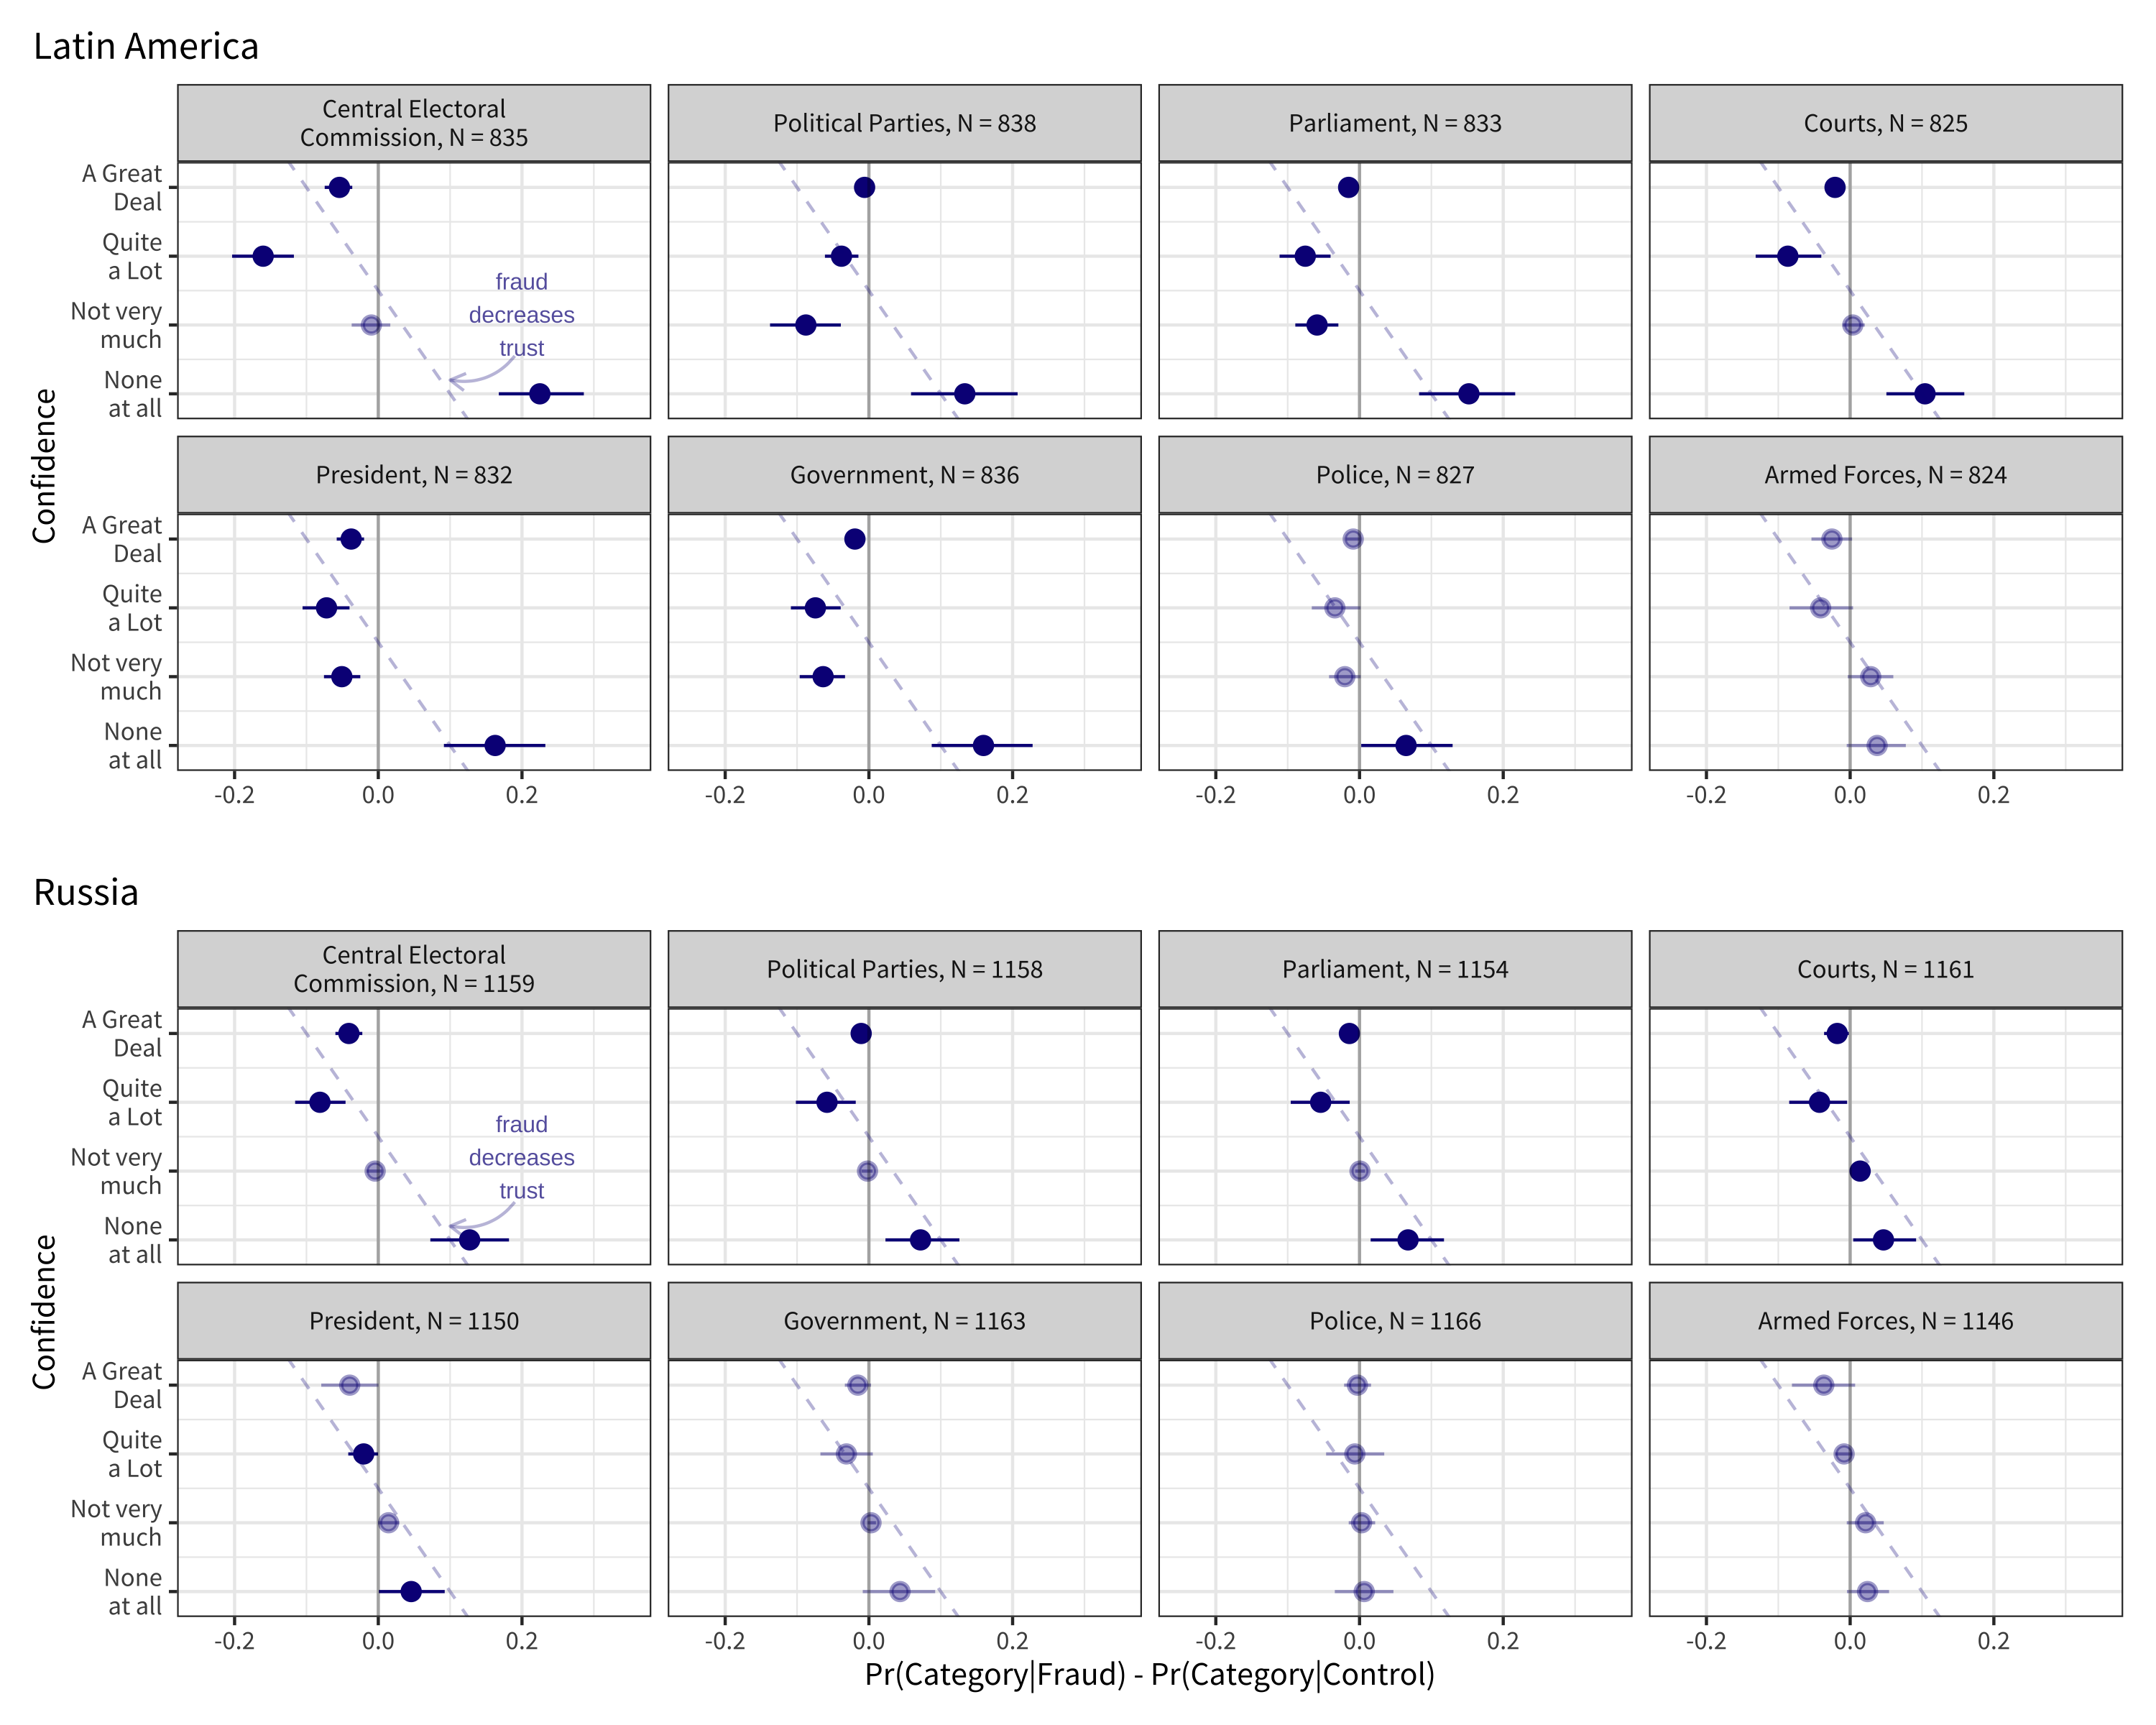
\includegraphics[width=\linewidth,trim=4 4 4 4,clip]{figs/main_hdi89_2.png}
	\caption{The Effects of Exposure to Fraud Information on Confidence in Political Institutions (samples exclude responses classified as irrelevant).  \\
		\footnotesize{Notes: Plots depict medians and 89\% highest-density continuous interval for differences in probabilities for choosing respective categories based on draws from the expectation of the posterior predictive distributions. Probabilities are calculated based on ordered logit model estimates.\\
			Positive values on the horizontal axis indicate that the probability of selecting a category is higher in fraud condition than in the other one. Conversely, negative values mean that respondent's probability to choose this was lower in fraud condition. Dashed line schematically depicts the hypothesized relationship between categories, i.e. point estimates would loosely follow the pattern of the dashed line if the relationship between trust and fraud information is as expected. Transparent point ranges include zero in the 89\% HDCI.\\
	} }
	\singlespacing
	\raggedright
	\label{fig:main-2}
\end{figure}
    
\begin{figure}[H]
	\centering
	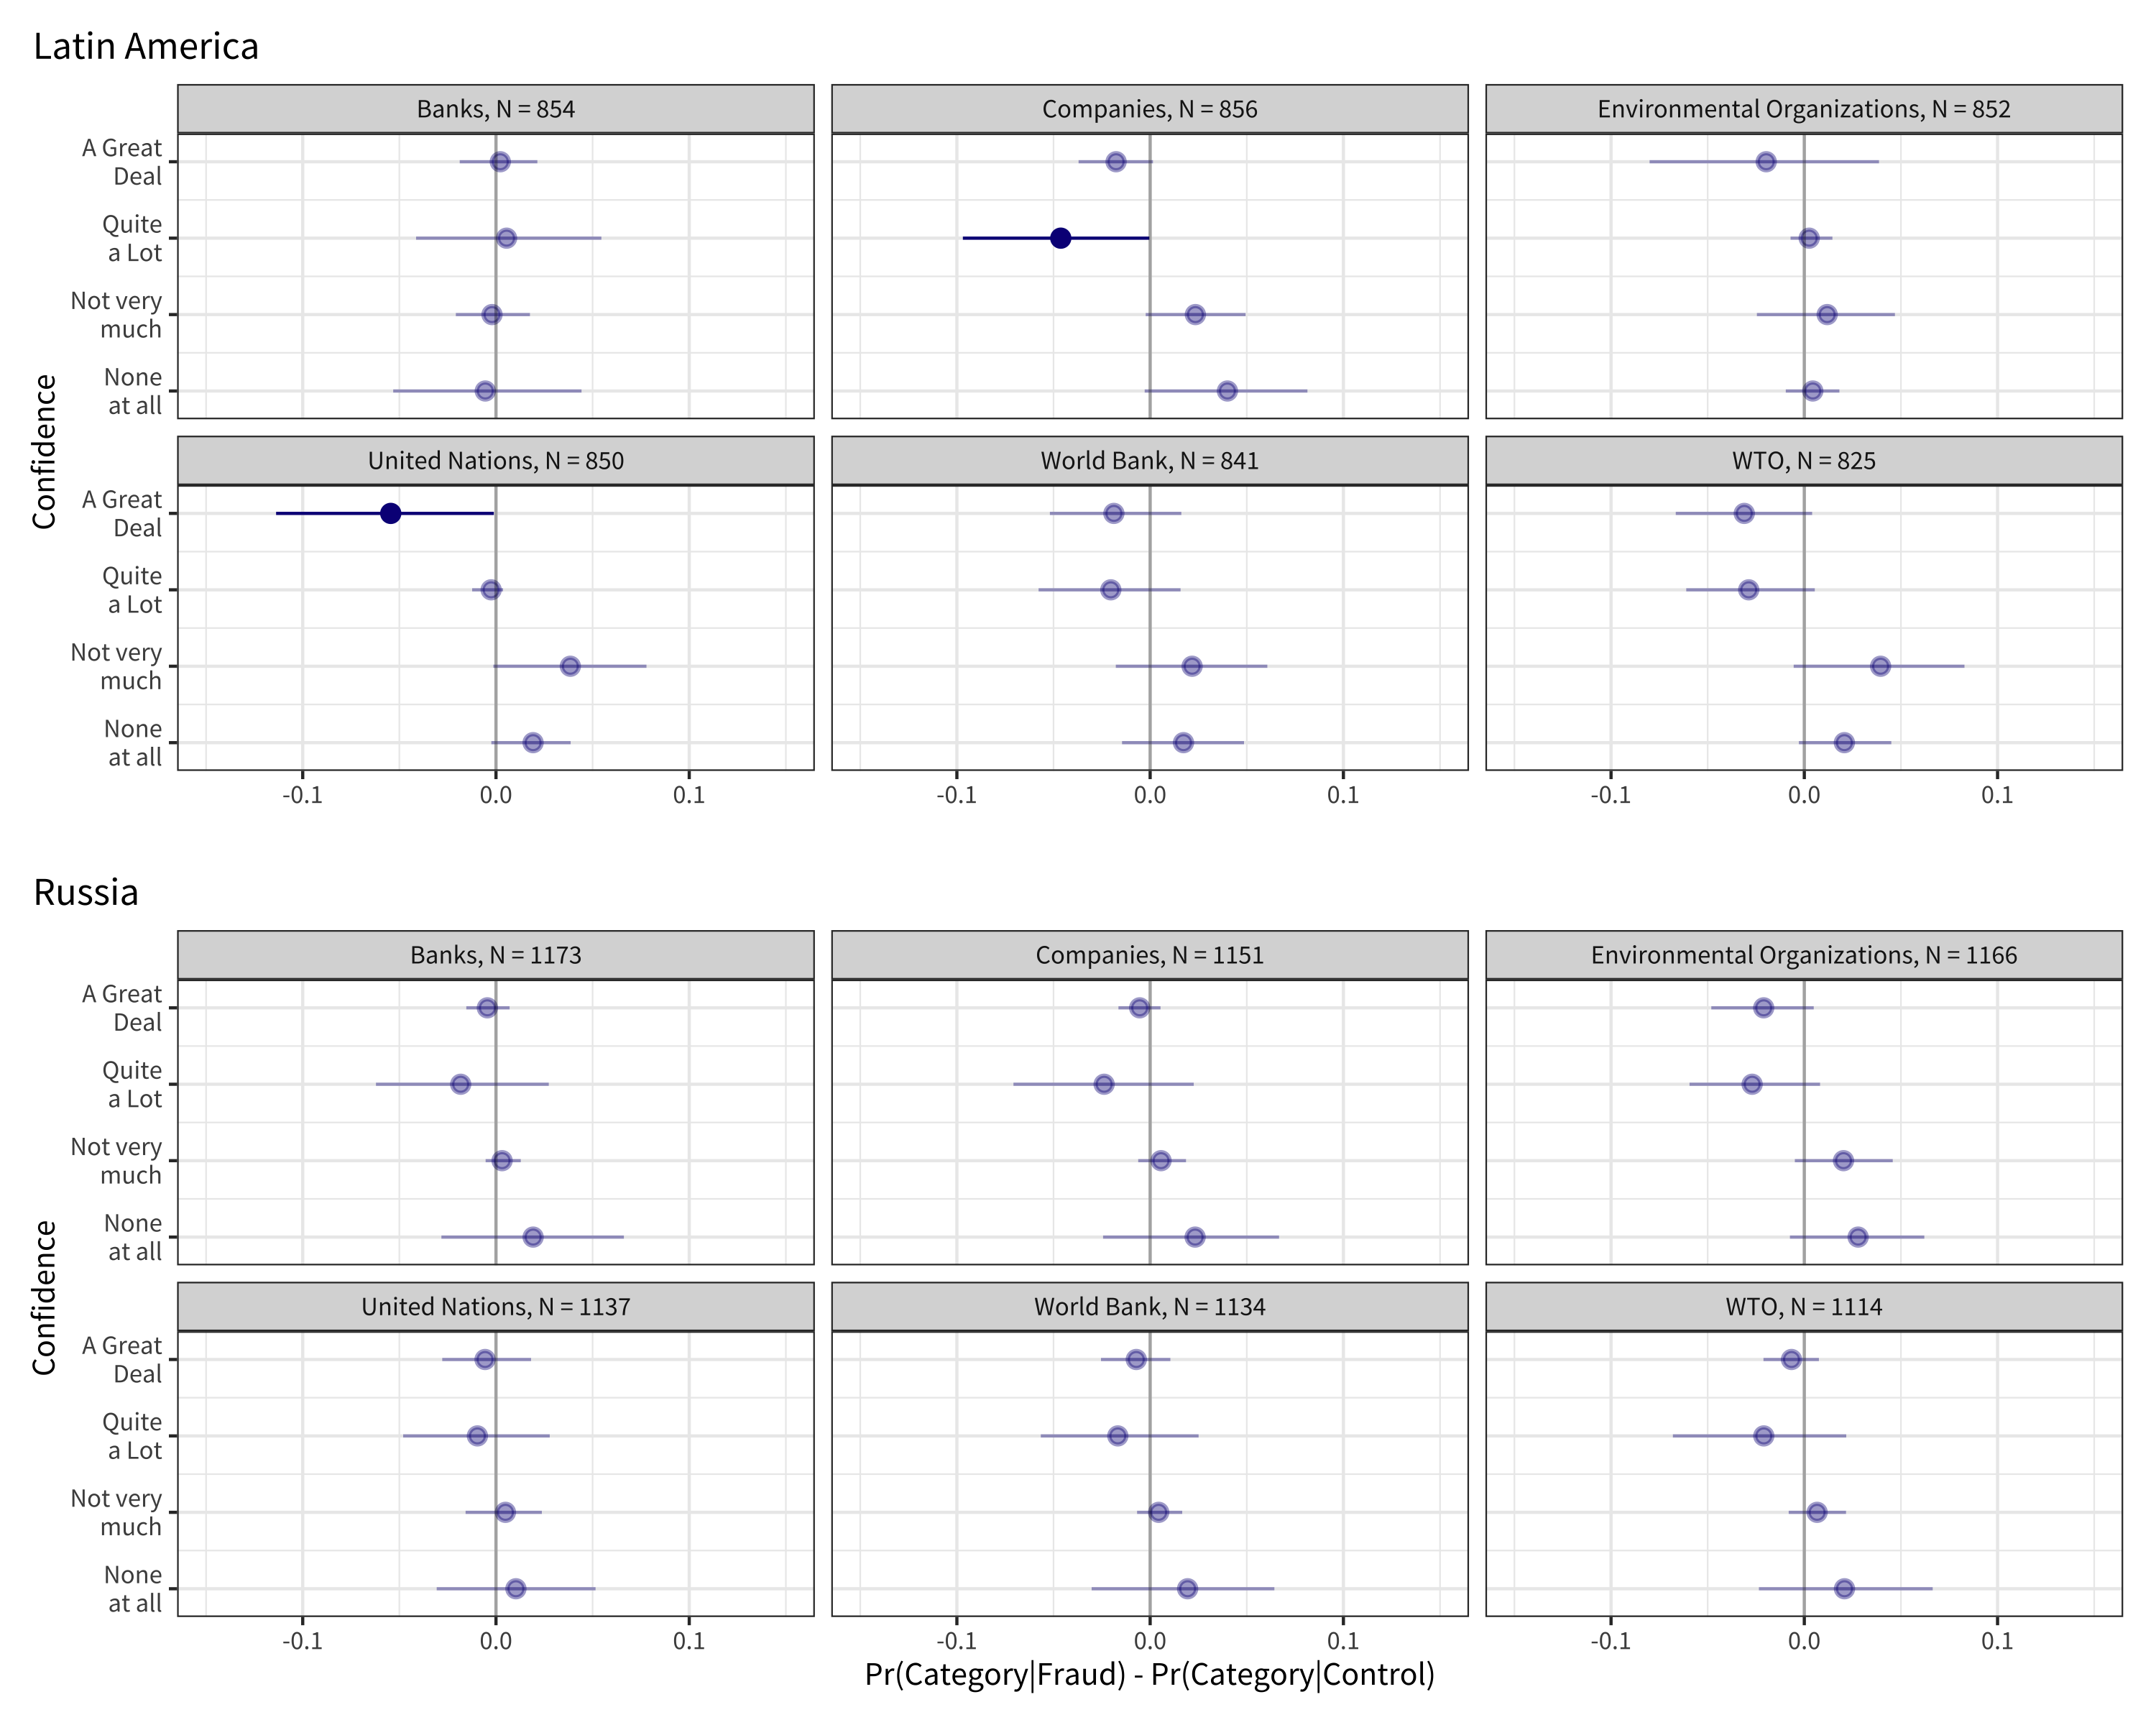
\includegraphics[width=\linewidth,trim=4 4 4 4,clip]{figs/main_hdi89_6.png}
	\caption{The Effects of Exposure to Fraud Information on Confidence in Non-political Institutions (samples exclude responses classified as irrelevant).  \\
		\footnotesize{Notes: Plots depict medians and 89\% highest-density continuous interval for differences in probabilities for choosing respective categories based on draws from the expectation of the posterior predictive distributions. Probabilities are calculated based on ordered logit model estimates.\\
			Positive values on the horizontal axis indicate that the probability of selecting a category is higher in fraud condition than in the other one. Conversely, negative values mean that respondent's probability to choose this was lower in fraud condition. Dashed line schematically depicts the hypothesized relationship between categories, i.e. point estimates would loosely follow the pattern of the dashed line if the relationship between trust and fraud information is as expected. Transparent point ranges include zero in the 89\% HDCI.\\
	} }
	\singlespacing
	\raggedright
	\label{fig:main-6}
\end{figure}
    
    
\clearpage

Furthermore, our manual coding of attention checks allowed us to closely examine the cases where the respondents seemed to have read the treatment text closely and in full, as their responses include the treatment-specific scenario details. For such individuals, we should observe strongest effects should our theory hold, though this effect could be counteracted by the fact of smaller sample sizes. Still, we observe stronger effects for more political institutions than in the full sample. In fact, we find strong evidence for the spillover effects of fraud in both countries for this subsample (figure \ref{fig:main-3}). At the same time, we also find some significant differences for banks and companies among the non-political institutions (figure \ref{fig:main-7}). However, the median value of size of these differences relative to medians for political institutions in this subsample is very modest, which still allows us to conclude that spillover effects occur to a varying extent for political institutions and entities with weaker connections to politics. 

\begin{figure}[H]
	\centering
	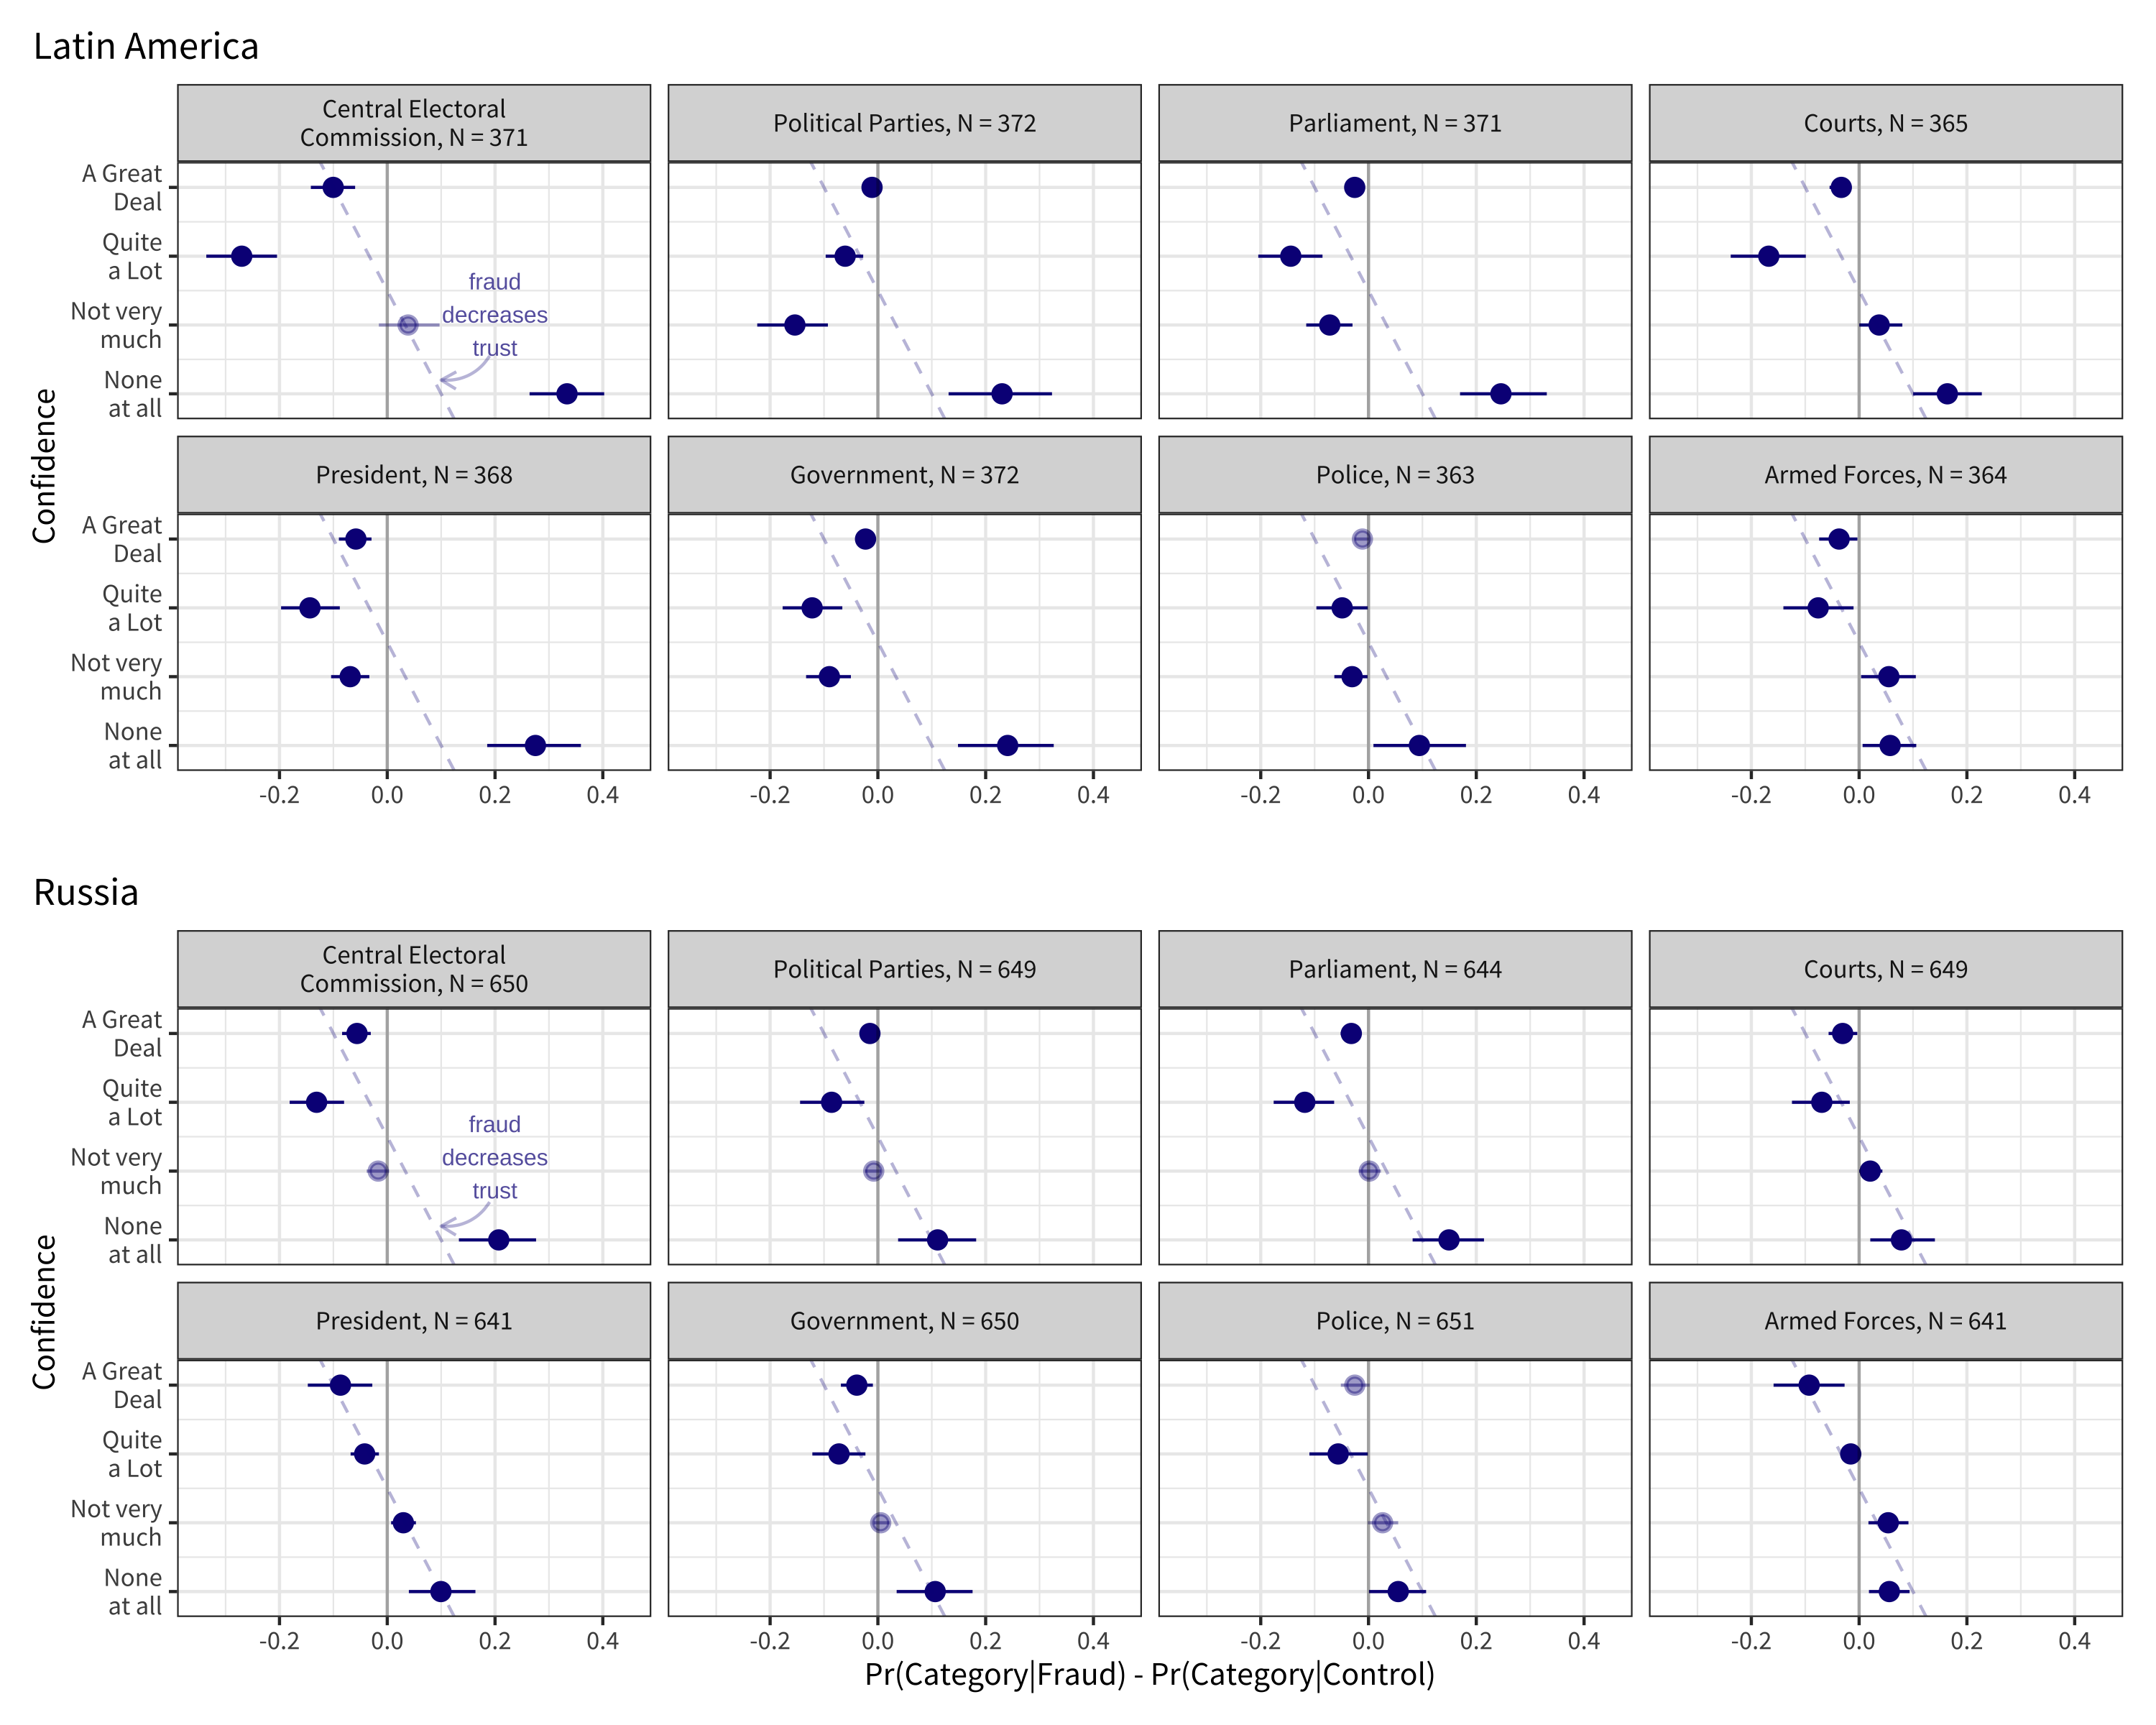
\includegraphics[width=\linewidth,trim=4 4 4 4,clip]{figs/main_hdi89_3.png}
	\caption{The Effects of Exposure to Fraud Information on Confidence in Political Institutions (only complete summaries of treatment texts).  \\
		\footnotesize{Notes: Plots depict medians and 89\% highest-density continuous interval for differences in probabilities for choosing respective categories based on draws from the expectation of the posterior predictive distributions. Probabilities are calculated based on ordered logit model estimates.\\
			Positive values on the horizontal axis indicate that the probability of selecting a category is higher in fraud condition than in the other one. Conversely, negative values mean that respondent's probability to choose this was lower in fraud condition. 
% 			Dashed line schematically depicts the hypothesized relationship between categories, i.e. point estimates would loosely follow the pattern of the dashed line if the relationship between trust and fraud information is as expected. 
Transparent point ranges include zero in the 89\% HDCI.\\
	} }
	\singlespacing
	\raggedright
	    
	\label{fig:main-3}
\end{figure}

\begin{figure}[H]
	\centering
	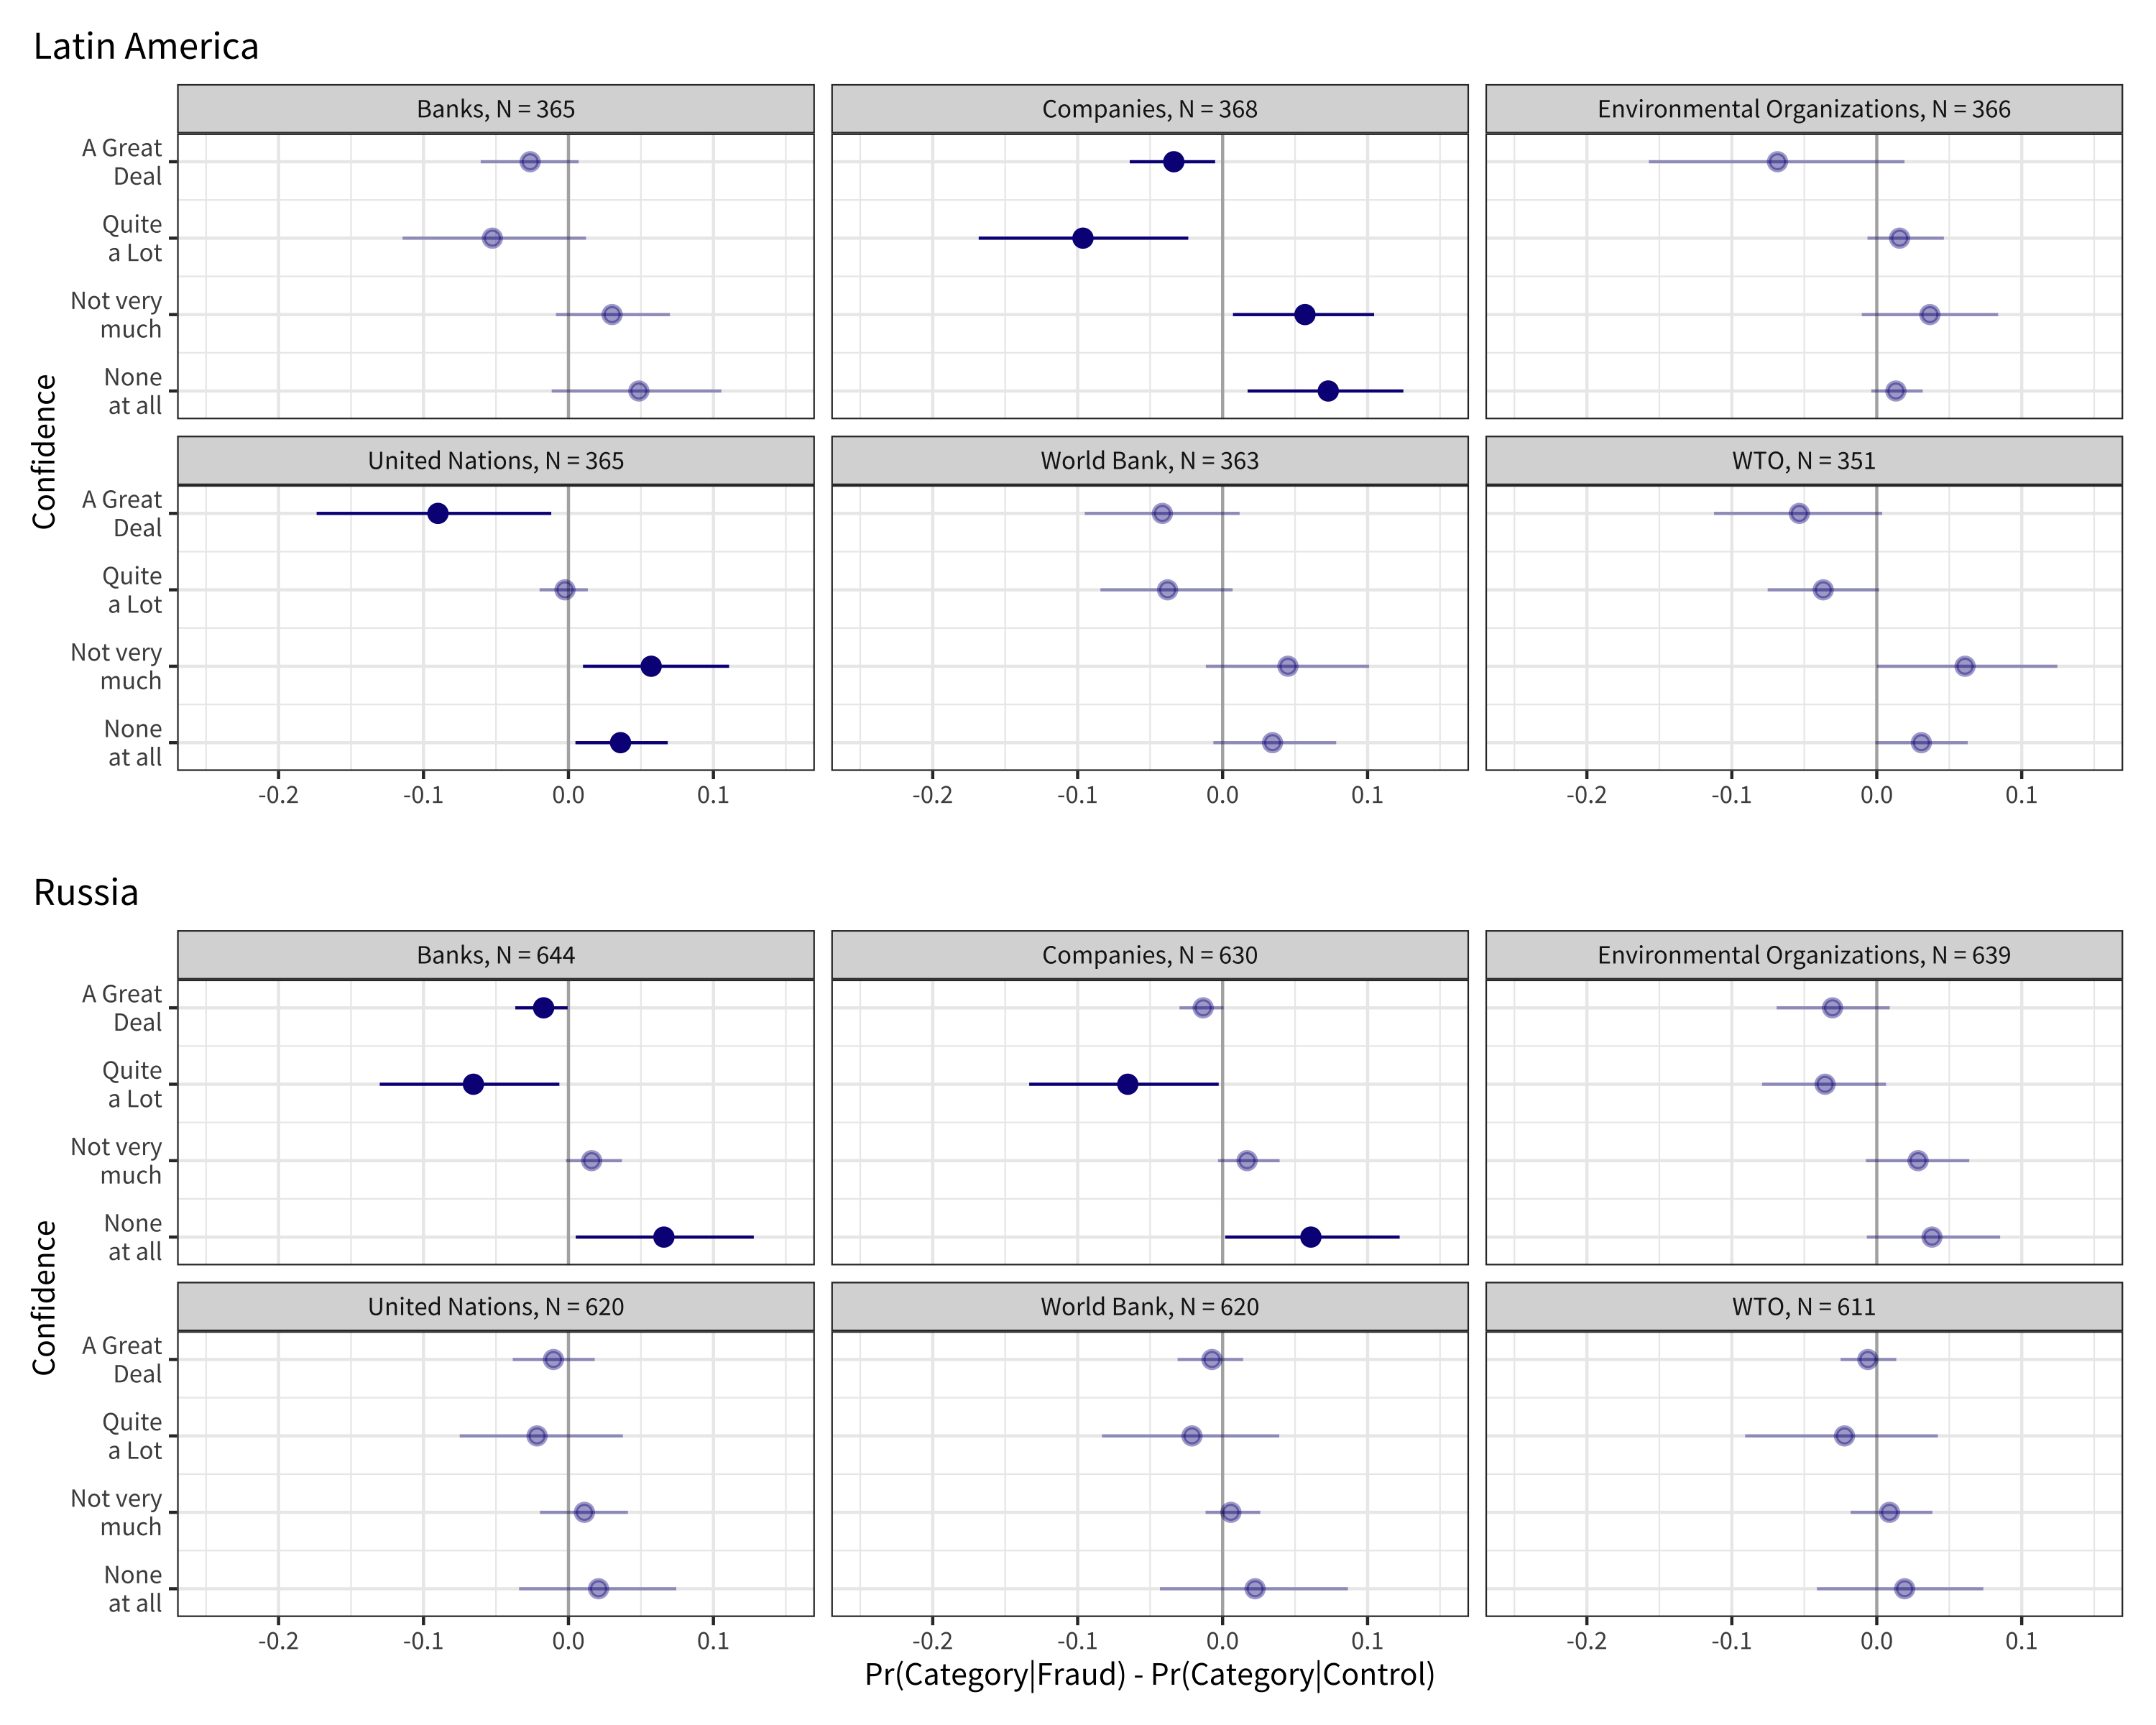
\includegraphics[width=\linewidth,trim=4 4 4 4,clip]{figs/main_hdi89_7.png}
	\caption{The Effects of Exposure to Fraud Information on Confidence in Non-political Institutions (only complete summaries of treatment texts).  \\
		\footnotesize{Notes: Plots depict medians and 89\% highest-density continuous interval for differences in probabilities for choosing respective categories based on draws from the expectation of the posterior predictive distributions. Probabilities are calculated based on ordered logit model estimates.\\
			Positive values on the horizontal axis indicate that the probability of selecting a category is higher in fraud condition than in the other one. Conversely, negative values mean that respondent's probability to choose this was lower in fraud condition. 
% 			Dashed line schematically depicts the hypothesized relationship between categories, i.e. point estimates would loosely follow the pattern of the dashed line if the relationship between trust and fraud information is as expected. 
Transparent point ranges include zero in the 89\% HDCI.\\
	} }
	\singlespacing
	\raggedright
	    
	\label{fig:main-7}
\end{figure}

% \subfile{tables/ol_main_la_npol_376}
% \subfile{tables/ol_main_ru_npol_667}

\clearpage
\subsection*{Subsample Analysis for Fraud Effect}

While our main hypothesis for fraud's effect refers to the complete sample, it may further help in exploring the heterogeneous effects of fraud for regime opponents and supporters, as we do with the punishment information. Given that our control condition is describing the status quo, it may prompt various associations for regime supporters, who are more likely to be treating status quo as a neutral state, and regime opponents, who may in fact perceive current state as resulting from the fraudulent practices. Hence, the observed effects of fraud in comparison to the control condition may in fact be primarily driven by the supporters' subgroups' responses, should they be updating their beliefs in response to treatment. Figures below illustrate this difference



    
\clearpage
\subsection*{Mediation Analysis}

\onehalfspacing
In this section we further investigate the mechanisms of attitudes' updating via mediation analysis. The spillover theory implies that it is the changes in trust in elections and electoral process that are responsible for the differences in the confidence in institutions of the political system. We thus have included a separate question that accounts for trust in election system after the treatment (the exact phrasing is: \textit{In this hypothetical scenario, how much confidence would you have in elections in [Mexico/Colombia/Russia]?}) We use answers to this question as a mediator to trace the effects of the fraud and punishment information on political attitudes. Figure below presents the argument graphically:

\begin{figure}[H]
	\centering
	\begin{tikzpicture}
		\node[mynode] (m){Confidence in Elections};
		\node[mynode,below left=of m](a) {Fraud/Punishment Information};
		\node[mynode,below right=of m](b) {Confidence in Institution};
		\draw[-latex] (a.north) -- node[auto,font=\footnotesize] { } (m.west);
		\draw[-latex] (m.east) -- node[auto,font=\footnotesize] { } (b.north);
		\draw[-latex, dotted] (a.east) --
		node[below=3mm,font=\footnotesize,align=center] {}
		(b.west);
	\end{tikzpicture}
\end{figure}

\noindent We estimate the ordered logit models specified as follows.

\noindent Outcome model:
\begin{equation}
	% \begin{split}
	\small
	ln \left (\frac{\text{Pr}(y_i \leq j)}{\text{Pr}(y_i > j)} \right) = \alpha_j - \underbrace{
		({\beta_1} {\text{ Control}_i} + 
		\beta_2 {\text{ Punishment}_i} + 
		\beta_3 {\text{ Judicial Punishment}_i})
		}_{\text{Treatment Variables}} +
	\underbrace{\beta_4 \text{ Trust in Elections}_i,}_{
		\text{Mediator}}
	% \end{split}
\end{equation}

\noindent Mediator model:
\begin{equation}
	% \begin{split}
	\small
	ln \left (\frac{\text{Pr}(\text{Trust in Elections}_i \leq j)}{\text{Pr}(\text{Trust in Elections}_i > j)} \right) =\gamma_j - 
	({\delta_1} {\text{ Control}_i} + 
	\delta_2 {\text{ Punishment}_i} + 
	\delta_3 {\text{ Judicial Punishment}_i})
\end{equation}


\noindent where $y_i$ is the level of diffuse support of an individual $i$ with ($i=1,...,n$) for an institution, and Control, Punishment, and Judicial Punishment are binary indicators for membership in the experimental groups (2),  (3), and (4) \footnote{Individuals who only received fraud information serve as the reference category in our analysis.}. Trust in Elections$_i$ is the level of trust in electoral process in the country and is on the same scale as the main outcome variable, institutional trust. As in the main analysis, we analyze Russian and Latin American samples separately, using all available observations that fulfill the basic data-quality criteria, such as completing the questionnaire in lower than 3 minutes.
    
For each political institution, we estimate an ordered logit model for trust in elections and model institutional trust using the estimates from the ordered logit in the previous step. It is our expectation that \textit{direct effect} of treatment on institutional trust, once the model includes trust in elections, is close to zero, while the indirect effect, the \textit{average causal mediation effect}, would be different from zero and positive: as trust categories are both measured on the same scale of 1 to 4, we should expect a positive relationship between them, and in comparison to fraud alone, status quo information and the punishment would be expected to raise the trust. Figure \ref{fig:mediation} presents the results of the analysis for Latin American and Russian samples. 

When we look at the effect of fraud information alone, we can observe that across all institutions, indirect effect, \textit{ACME}, is significantly different from zero and positive, which is in line with our expectations: increased (decreased) trust in elections is associated with increased (decreased) trust in political institutions. At the same time, the direct effect, i.e. the effect of treatment alone on confidence in institutions, is for most institutions, not different from zero, meaning that most of the changes in institutional confidence in response to treatment seem to be driven by the declines in trust in the elections. For the punishment information, we only observe the effects of treatment once the courts are reported to intervene , and the effect again is primarily existing via trust in elections. For punishment information alone, with no judicial intervention, we observe only the relationship between the trust in elections and trust in 

\begin{figure}[H]
	\centering
	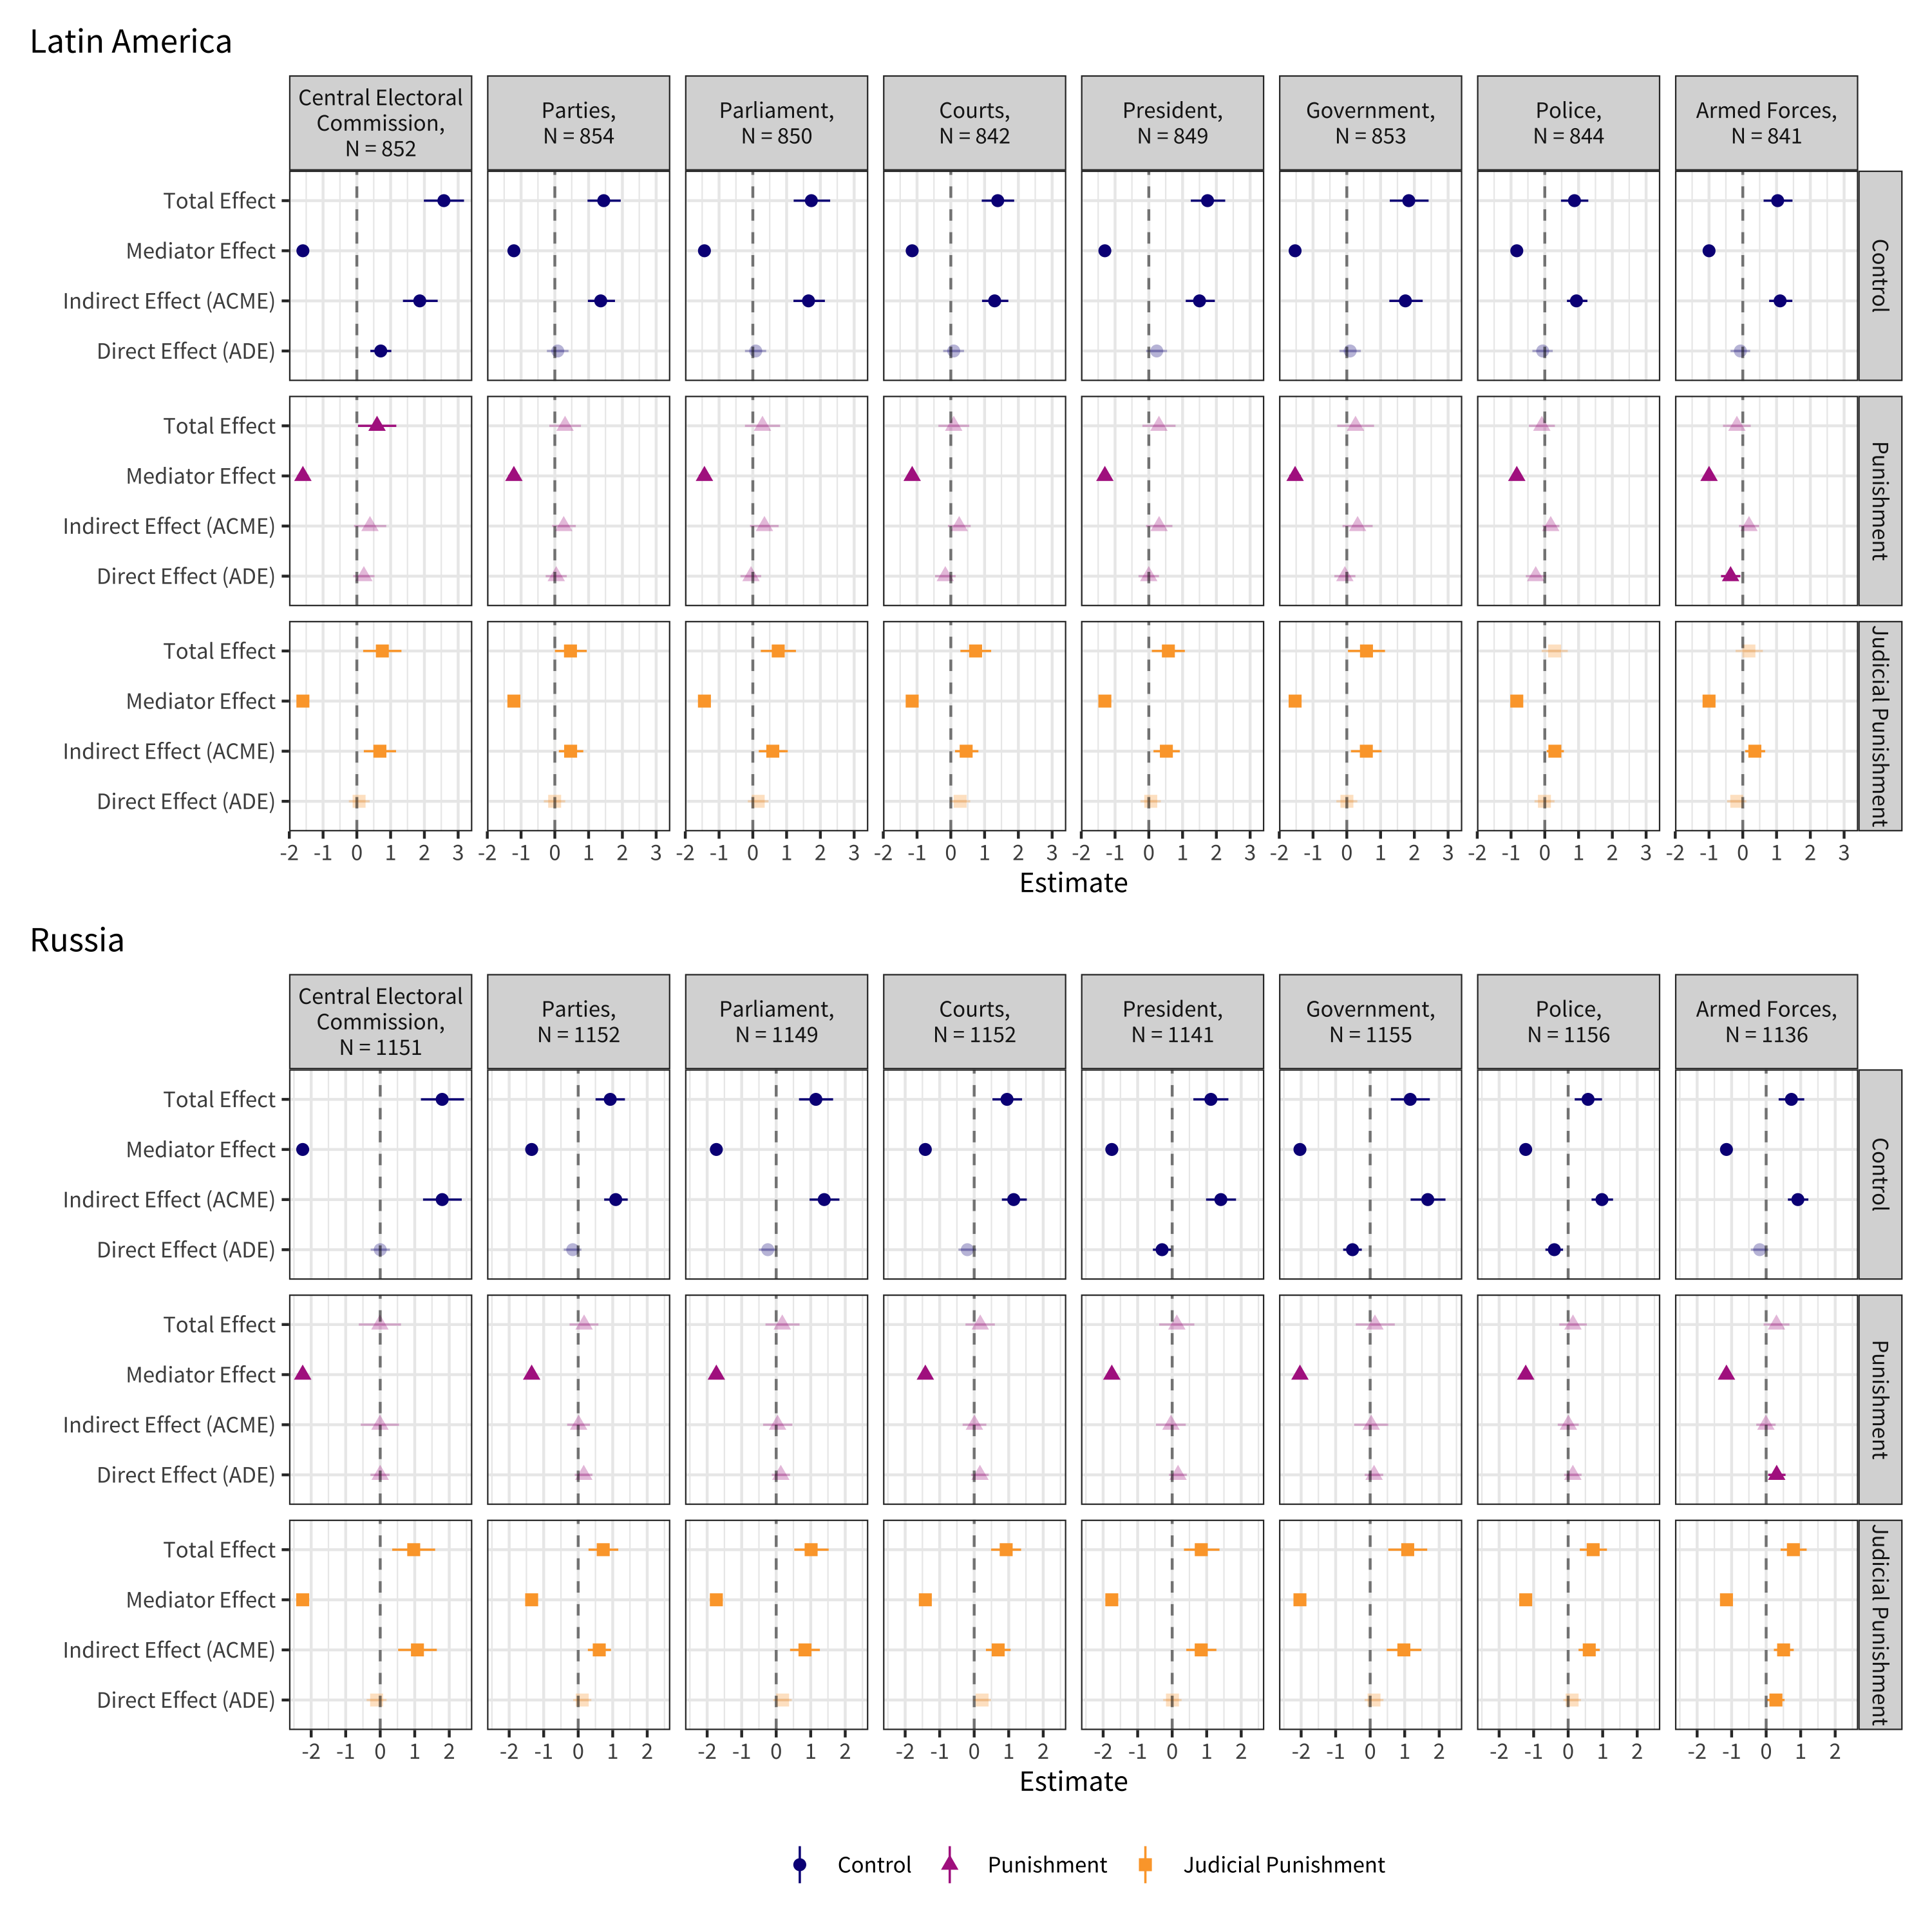
\includegraphics[width=\linewidth,trim=4 4 4 4,clip]{figs/mediation.png}
	\caption{The Results of Mediation Analysis.  \\
		\footnotesize{Notes: Depicted are the \textit{direct effect }(median value and 89\% highest-density continuous interval (HDCI) of posterior samples from treatment of the institutional trust model), \textit{mediator effect} (median value and 89\% HDCI of posterior samples from mediator, trust in elections, of the institutional trust model), \textit{indirect effect} (median value and 89\% HDCI of the multiplication of the posterior samples from mediator, trust in elections,  of the institutional trust model and the posterior samples from treatment of the trust in elections' model) and the \textit{total effect} (median value and 89\% HDCI of sums of posterior samples used for the direct and indirect effect).  } 
	}
	\singlespacing
	\raggedright
	\label{fig:mediation}
\end{figure}

\clearpage
\subsection*{Models with Controls}

This section contains tables with estimates for the models from our survey experiment, but this time with control variables (tables \ref{table:ol-controls-la-pol-881} and \ref{table:ol-controls-ru-pol-1226}). While random assignment allows us to drop the controls in our main analysis (for balance assessment across groups see tables \ref{descr:la} and \ref{descr:russia}), we replicate the results using control variables as well. We use sociodemographic (measured post-treatment) and political attitudes (measured pre-treatment) variables. We have attempted to include the same variables as in our matching analysis for the sake of uniformity and, to a certain extent, comparability. We thus control for 
\begin{itemize}
	\item \textit{generalized trust}, as it may be directly related to confidence in political system institutions; 
	\item \textit{political interest}, as we may expect a relationship between trust and investment into the topic with causal effects pointing in either direction; 
	\item \textit{political affiliation}, as opposition to the regime may decrease trust in its institutions as of itself; 
	\item \textit{age (logged)}, as we may expect younger respondents to show less trust to political institutions;
	\item \textit{education}, as it may proxy the critical thinking skills and potentially, differences in degrees of sophistication in the evaluations; 
	\item \textit{employment status}, as it may impact the overall government performance evaluation as well as impact the socialisation and information channels available to respondents; 
	\item \textit{employment sector}, as working for the government may be associated with changes in political attitudes (CITE ROSENFELD);
	\item \textit{savings}, as economic security and income are known to impact the performance of (and, potentially, trust in) government institutions;
	\item \textit{political corruption}, as perceptions of corruption are likely directly related to trust in political institutions.
\end{itemize}
None of these variables are expected to be systematically related to the treatment variables due to random assignment. As a result, the estimates differ marginally with their significance and signs, and follow the patterns we observe in the main analysis.


\clearpage
\subfile{tables/ol_controls_la_pol_881}

\clearpage

\subfile{tables/ol_controls_ru_pol_1226}


\subsection*{Alternative Specifications for Regime Opposition Variable}

In Russia, one could argue that only UR partisans should be treated as supporters, hence we replicate the analysis with this definition as well as explore further distinctions between non-partisans and partisans. 


\subsection*{Political Interest Suppresses the Effects of Spillover}
\subsection*{Education Suppresses the Effects of Spillover}

\subsection*{News Consumption Source}


\subsection*{Models with Expected Involvement of Officials}


\section*{Questionnaire and Translations}




% \vspace{0.5cm}

% \begin{center}
%     POLITICAL ATTITUDES \\
% \end{center}

% \noindent \textbf{INT}. How interested would you say you are in politics? \\
% (1) A lot \\
% (2) Some \\
% (3) Little \\
% (4) None \\

% \noindent \textbf{PID1}. Do you currently identify with a political party? \\
% (1) Yes \\
% (2) No \\
% (99) Don't know / Refusal \\

% \noindent \textbf{PID2}. Which political party do you identify with? \\
% \noindent [INSERT HERE] \\

% \noindent \textbf{VOTE1}. Did you vote in the last presidential elections of [year of last presidential elections]? \\
% (1) Voted \\
% (2) Did not vote \\
% (99) Don't know / Refusal \\

% \noindent \textbf{VOTE2}. If there were a national legislative election tomorrow, for which party on this list would you vote? \\ \noindent [LIST OPTIONS HERE] \\

% \noindent \textbf{LR}. Below you see portrayed a 1-10 scale that goes from left to right. The number one means left and 10 means right. Nowadays, when we speak of political leanings, we talk of those on the left and those on the right. In other words, some people sympathize more with the left and others with the right. According to the meaning that the terms "left" and "right" have for you, and thinking of your own
% political leanings, where would you place yourself on this scale? \\

% \noindent (1) \hspace{0.1cm} (2) \hspace{0.1cm} (3) \hspace{0.1cm} (4) \hspace{0.1cm} (5) \hspace{0.1cm} (6) \hspace{0.1cm} (7) \hspace{0.1cm} (8) \hspace{0.1cm} (9) \hspace{0.1cm} (10) \\
% Left \hspace{6cm} Right \\

% \noindent (99) Don't know / Refusal \\

% \newpage

% \noindent \textbf{CORRUP}. Now please let us know your views on corruption – when people pay a bribe, give a gift or do a favor to other people in order to get the things they need done or the services they need. How would you place your views on corruption in your country on a 10-point scale where “1” means “there is no corruption in my country” and “10” means “there is abundant corruption in my country”. If your views are somewhat mixed, choose the appropriate number in between. \\

% \noindent (1) \hspace{0.1cm} (2) \hspace{0.1cm} (3) \hspace{0.1cm} (4) \hspace{0.1cm} (5) \hspace{0.1cm} (6) \hspace{0.1cm} (7) \hspace{0.1cm} (8) \hspace{0.1cm} (9) \hspace{0.1cm} (10) \\
% No courruption \hspace{6cm} Abundant corruption \\

% \noindent (99) Don't know / Refusal \\



% \noindent \textbf{INTERT}. And speaking of the people from around here, would you say that people in this community are very trustworthy, somewhat trustworthy, not very trustworthy or
% untrustworthy? \\
% (1) Very trustworthy \\
% (2) Somewhat trustworthy \\
% (3) Not very trustworthy \\
% (4) Untrustworthy \\
% (99) Don't know / Refusal \\

% \vspace{1cm}

% \begin{center}
%     TREATMENT AND OUTCOME
% \end{center}

% \noindent \textbf{SPLIT Control Group: Neutral Information} \\
% On Sunday, \textit{[6 June 2021/19 September 2021]}, legislative elections are scheduled to be held in \textit{[Mexico/Russia]}. More than 2,000 registered candidates will compete for the \textit{[500/450]} parliamentary seats of the \textit{[Champer of Deputies/State Duma]}. The results will be determined by nearly \textit{[90/110]} million people in \textit{[Mexico/Russia]} and abroad. Suppose that as in the current convocation, \textit{[seven/four]} parties retained positions. \\

% %Suppose that federal legislative elections for the \textit{[Champer of Deputies/State Duma]} were held in \textit{[month]} of this year. Imagine that as usual, also in this hypothetical election more than 2,000 candidates competed for the \textit{[500/450]} parliamentary seats. Suppose that all parties that are currently presented in the \textit{[Champer of Deputies/State Duma]} have retained positions in the assembly and that the incumbent party \textit{[MORENA/United Russia]} has won the largest seat share. \\ as in the current convocation/parliament7as currently, four/seven parties retained positions. 

% \noindent \textbf{SPLIT Treatment Group: Fraud Information} \\
% \hl{$[$Neutral information$]$} \\
% On an after election day, however, allegations of ballot-box stuffing and alterations of vote tallies perpetrated by individuals working for electoral commissions in favor of the incumbent party were widespread. Shortly after election day, a number of domestic and international election observation missions publicly called out a variety of electoral misconducts and manipulation practices across several regions of the country. \\

% \noindent \textbf{SPLIT Treatment Group: Fraud Information With Electoral Commission Punishment} \\
% \hl{$[$Neutral information$]$} \\
% \hl{$[$Fraud information$]$} \\
% As a consequence, individuals allegedly responsible for fraud lost their position in the electoral commissions that they served in. \\

% \newpage

% \noindent \textbf{SPLIT Treatment Group: Fraud Information With Court Punishment} \\
% \hl{$[$Neutral information$]$} \\
% \hl{$[$Fraud information$]$} \\
% As a consequence, legal action was brought against individuals allegedly responsible for fraud which were convicted for electoral crimes by responsible courts. \\

% \vspace{1cm}

% \noindent Upon receiving this information, how much confidence would you have in the following organizations or institutions? Below you see a ladder with steps numbered 1 to 7, where 1 is the lowest step and means NOT AT ALL and 7 the highest and means A LOT. The ladder is followed by a series of questions. Please use the numbers provided in the ladder to answer. Remember, you can use any number. \\

% \noindent (1) \hspace{1cm} (2) \hspace{1cm} (3) \hspace{1cm} (4) \hspace{1cm} (5) \hspace{1cm} (6) \hspace{1cm} (7) \\
% Not at all \hspace{8cm} A lot \\

% \noindent (99) Don't know / Refusal \\

% \vspace{0.5cm}

% \noindent \textbf{TRUST1}. To what extent do you trust the Armed Forces? \\

% \noindent \textbf{TRUST2}. To what extent do you trust the Police? \\

% \noindent \textbf{TRUST3}. To what extent do you trust the Electoral Commission? \\

% \noindent \textbf{TRUST4}. To what extent do you trust the Justice System/Courts? \\

% \noindent \textbf{TRUST5}. To what extent do you trust the Government? \\
 
% \noindent \textbf{TRUST6}. To what extent do you trust the Parliament? \\
 
% \noindent \textbf{TRUST7}. To what extent do you trust the Political Parties? \\

% \vspace{0.5cm}

% \noindent \textbf{INVOLVE.} Some people say that there are systematic irregularities to be observed in the federal elections of [country], while other people deny that. Given that such claims were true, to which extent do you expect representatives of political parties and state-affiliated agents to be involved?”. \\
% (1) Very involved \\
% (2) Somewhat involved \\
% (3) Not very involved \\
% (4) Not at all involved \\
% (99) Don't know / Refusal \\

% \newpage

% \begin{center}
%     SOCIO-DEMOGRAPHICS \\
% \end{center}

% \noindent \textbf{SEX}. What sex are you? \\
% (1) Female (2) Male (99) Don't know / Refusal \\

% \noindent \textbf{URBAN}. Which size is the place you live at? \\
% (1) National capital (metropolitan area) \\
% (2) Large city ($>$ 500,000) \\
% (3) Medium city ($>$ 100,000) \\
% (4) Small city ($>$ 20,000) \\
% (5) Rural area \\
% (99) Don't know / Refusal \\

% \noindent \textbf{BIRTH.} Can you tell me your year of birth, please? \\

% \noindent \textbf{AGE}. This means you are ... years old. \textit{(write age in two digits)} \\

% \noindent \textbf{IMMIG.} Were you born in this country or are you an immigrant to this country?  \\

% \noindent \textbf{CITIZ.} Are you a citizen of this country? \\	

% \noindent \textbf{EDU1}. What is the highest level of education you have attained? \\
% (0) Early childhood education (ISCED 0) / no education  \\
% (1) Primary education (ISCED 1) \\
% (2) Lower secondary education (ISCED 2) \\
% (3) Upper secondary education (ISCED 3) \\
% (4) Post-secondary non-tertiary education (ISCED 4) \\
% (5) Short-cycle tertiary education (ISCED 5) \\
% (6) Bachelor or equivalent (ISCED 6) \\
% (7) Master or equivalent (ISCED 7) \\
% (8) Doctoral or equivalent (ISCED 8) \\
% (99) Don't know / Refusal \\

% \noindent \textbf{EDU2}. About how many years of education have you completed, whether full-time or part-time? Please report these in full-time equivalents and include compulsory years of schooling. \\
% \noindent [INSERT HERE] \\

% \noindent \textbf{OCCUP}. Which of these descriptions \underline{best} describes your current situation? \\
% (1) In paid work (or away temporarily) (employee, self-employed, working for your family business) \\
% (2) In education, (not paid for by employer) even if on vacation \\
% (3) Unemployed and actively looking for a job 
% (4) Unemployed, wanting a job but not actively looking for a job \\
% (5) Permanently sick or disabled \\
% (6) Retired \\
% (7) In community or military service \\
% (8) Doing housework, looking after children or other persons 
% (9) Other \\
% (99) Don't know / Refusal \\

% \noindent \textbf{SECTOR}. Are you working for the government or public institution, for private business or industry, or for a private non-profit organization? If you do not work currently, characterize your major work in the past! Do you or did you work for: \\ 
% (1) Government or public institution \\
% (2)	Private business or industry \\
% (3)	Private non-profit organization \\ 

% \noindent \textbf{INC}. Which of the following descriptions comes closest to how you feel about your household's income nowadays? \\
% (1) Living comfortably on present income \\
% (2) Coping on present income \\
% (3) Finding it difficult on present income \\
% (4) Finding it very difficult on present income \\
% (99) Don't know / Refusal \\

\end{document}